\def\year{2021}\relax
%File: formatting-instructions-latex-2021.tex
%release 2021.2
\documentclass[letterpaper]{article} % DO NOT CHANGE THIS

\usepackage{aaai21}  % DO NOT CHANGE THIS
% \usepackage{aaai21_no_copyright}  % DO NOT CHANGE THIS  % XXX only for arXiv
\usepackage{soul}
\usepackage{times}  % DO NOT CHANGE THIS
\usepackage{helvet} % DO NOT CHANGE THIS
\usepackage{courier}  % DO NOT CHANGE THIS
\usepackage[hyphens]{url}  % DO NOT CHANGE THIS
\usepackage{graphicx} % DO NOT CHANGE THIS
\urlstyle{rm} % DO NOT CHANGE THIS
\def\UrlFont{\rm}  % DO NOT CHANGE THIS
\usepackage{natbib}  % DO NOT CHANGE THIS AND DO NOT ADD ANY OPTIONS TO IT
\usepackage{caption} % DO NOT CHANGE THIS AND DO NOT ADD ANY OPTIONS TO IT
\frenchspacing  % DO NOT CHANGE THIS
\setlength{\pdfpagewidth}{8.5in}  % DO NOT CHANGE THIS
\setlength{\pdfpageheight}{11in}  % DO NOT CHANGE THIS
\setlength{\belowcaptionskip}{-5pt}
% \setlength\abovecaptionskip{-0.25pt}
%\nocopyright
%PDF Info Is REQUIRED.
% For /Author, add all authors within the parentheses, separated by commas. No accents or commands.
% For /Title, add Title in Mixed Case. No accents or commands. Retain the parentheses.
\pdfinfo{
/Title (PLGRIM: Hierarchical Value Learning for Large-scale Autonomous Exploration in Unknown Environments)
/Author (Sung-Kyun Kim*, Amanda Bouman*, Gautam Salhotra, David D. Fan, Kyohei Otsu, Joel Burdick, Ali-akbar Agha-mohammadi)
/TemplateVersion (2021.2)
} %Leave this

% DISALLOWED PACKAGES
% \usepackage{authblk} -- This package is specifically forbidden
% \usepackage{balance} -- This package is specifically forbidden
% \usepackage{color (if used in text)
% \usepackage{CJK} -- This package is specifically forbidden
% \usepackage{float} -- This package is specifically forbidden
% \usepackage{flushend} -- This package is specifically forbidden
% \usepackage{fontenc} -- This package is specifically forbidden
% \usepackage{fullpage} -- This package is specifically forbidden
% \usepackage{geometry} -- This package is specifically forbidden
% \usepackage{grffile} -- This package is specifically forbidden
% \usepackage{hyperref} -- This package is specifically forbidden
% \usepackage{navigator} -- This package is specifically forbidden
% (or any other package that embeds links such as navigator or hyperref)
% \indentfirst} -- This package is specifically forbidden
% \layout} -- This package is specifically forbidden
% \multicol} -- This package is specifically forbidden
% \nameref} -- This package is specifically forbidden
% \usepackage{savetrees} -- This package is specifically forbidden
% \usepackage{setspace} -- This package is specifically forbidden
% \usepackage{stfloats} -- This package is specifically forbidden
% \usepackage{tabu} -- This package is specifically forbidden
% \usepackage{titlesec} -- This package is specifically forbidden
% \usepackage{tocbibind} -- This package is specifically forbidden
% \usepackage{ulem} -- This package is specifically forbidden
% \usepackage{wrapfig} -- This package is specifically forbidden
% DISALLOWED COMMANDS
% \nocopyright -- Your paper will not be published if you use this command
% \addtolength -- This command may not be used
% \balance -- This command may not be used
% \baselinestretch -- Your paper will not be published if you use this command
% \clearpage -- No page breaks of any kind may be used for the final version of your paper
% \columnsep -- This command may not be used
% \newpage -- No page breaks of any kind may be used for the final version of your paper
% \pagebreak -- No page breaks of any kind may be used for the final version of your paperr
% \pagestyle -- This command may not be used
% \tiny -- This is not an acceptable font size.
% \vspace{- -- No negative value may be used in proximity of a caption, figure, table, section, subsection, subsubsection, or reference
% \vskip{- -- No negative value may be used to alter spacing above or below a caption, figure, table, section, subsection, subsubsection, or reference

% \setcounter{secnumdepth}{0} %May be changed to 1 or 2 if section numbers are desired.
\setcounter{secnumdepth}{2} %May be changed to 1 or 2 if section numbers are desired.


\graphicspath{{../}{./}{./figures/}}


%%%%%%%%%%%%%%%%%%%%%%%%%%%%%%%%%%%%%%%
%%%%%%%%%%%%%%%%%%%%%%%%%%%%%%%%%%%%%%%

\usepackage[utf8]{inputenc}
\usepackage[T1]{fontenc}
\usepackage{graphicx}
\usepackage{float}
\usepackage{xcolor}
\usepackage[normalem]{ulem}
\usepackage[justification=centering]{subfig}

\usepackage{amsmath}
\usepackage{amsfonts}
\usepackage{amssymb}
\usepackage{mathtools}
\usepackage{todonotes}
\usepackage{enumitem}
\usepackage{multicol}
\usepackage{comment}
% \usepackage[noend]{algpseudocode} % this breaks my algorithm box

\usepackage{tikzpagenodes}

% \usepackage[
%   subtle
%   %moderate
% ]{savetrees}

\usepackage{algorithm,algorithmic}

\newcommand{\ph}[1]{{\textbf{#1}:}} % paragraph header
% \newcommand{\phdone}[1]{{\textbf{#1}:}} % (invisible) paragraph header
\newcommand{\phdone}[1]{} % (invisible) paragraph header
\newcommand{\ncomment}[1]{}
\newcommand{\acomm}[1]{{\color{cyan}Ali:#1}} % Ali's comments from video
\newcommand{\qcomm}[1]{{\color{red}Quest.}} % Ali's comments from video
% \newcommand{\todo}[1]{{\color{red} #1 }} % Tasks to do
\newcommand{\note}[1]{{\color{red}#1 }}
\newcommand{\maximize}{\mathop{\mathrm{maximize}}}
\newcommand{\argmax}{\mathop{\mathrm{argmax}}}
\newcommand{\argmin}{\mathop{\mathrm{argmin}}}

%%%%%%%%%%%%%%%%%%%%%%%%%%%%%%%%%%%%%%%
%%%%%%%%%%%%%%%%%%%%%%%%%%%%%%%%%%%%%%%



% The file aaai21.sty is the style file for AAAI Press
% proceedings, working notes, and technical reports.
%

% Title

% Your title must be in mixed case, not sentence case.
% That means all verbs (including short verbs like be, is, using,and go),
% nouns, adverbs, adjectives should be capitalized, including both words in hyphenated terms, while
% articles, conjunctions, and prepositions are lower case unless they
% directly follow a colon or long dash

\title{
    PLGRIM: Hierarchical Value Learning for \\Large-scale Autonomous Exploration in Unknown Environments
		% PLGRIM: Hierarchical Value Learning for \underline{Real-world} \\Large-scale \sout{Autonomous} Exploration in Unknown Environments
}
\author{
		Sung-Kyun Kim,\thanks{These authors contributed equally to this work.}\textsuperscript{\rm 1}
		% Sung-Kyun Kim,\thanks{These authors contributed equally to this work. \newline \hspace*{1.1em} \copyright2021. All rights reserved.}\textsuperscript{\rm 1}  % XXX only for arXiv
    Amanda Bouman,$^{*}$\textsuperscript{\rm 2}
    Gautam Salhotra,\textsuperscript{\rm 3}
    David D. Fan,\textsuperscript{\rm 1} \\
    Kyohei Otsu,\textsuperscript{\rm 1}
    Joel Burdick,\textsuperscript{\rm 2}
    Ali-akbar Agha-mohammadi\textsuperscript{\rm 1} \\
}
\affiliations{
    \textsuperscript{\rm 1}
    NASA Jet Propulsion Laboratory,
    California Institute of Technology
    \\ \{sung.kim,
    david.d.fan,
    kyohei.otsu,
    aliagha\}\!@jpl.nasa.gov
    % \\ aliakbar.aghamohammadi@jpl.nasa.gov
    \\
    \textsuperscript{\rm 2}
    Department of Mechanical and Civil Engineering,
    California Institute of Technology
    \\ abouman@caltech.edu,
    jwb@robotics.caltech.edu
    \\
    \textsuperscript{\rm 3}
    Department of Computer Science,
    University of Southern California
    \\ salhotra@usc.edu
}
% \author{
%     %Authors
%     % All authors must be in the same font size and format.
%     Written by AAAI Press Staff\textsuperscript{\rm 1}\thanks{With help from the AAAI Publications Committee.}\\
%     AAAI Style Contributions by Pater Patel Schneider,
%     Sunil Issar,  \\
%     J. Scott Penberthy,
%     George Ferguson,
%     Hans Guesgen,
%     Francisco Cruz,
%     Marc Pujol-Gonzalez
%     \\
% }
% \affiliations{
%     %Afiliations
%     \textsuperscript{\rm 1}Association for the Advancement of Artificial Intelligence\\
%     %If you have multiple authors and multiple affiliations
%     % use superscripts in text and roman font to identify them.
%     %For example,
%
%     % Sunil Issar, \textsuperscript{\rm 2}
%     % J. Scott Penberthy, \textsuperscript{\rm 3}
%     % George Ferguson,\textsuperscript{\rm 4}
%     % Hans Guesgen, \textsuperscript{\rm 5}.
%     % Note that the comma should be placed BEFORE the superscript for optimum readability
%
%     2275 East Bayshore Road, Suite 160\\
%     Palo Alto, California 94303\\
%     % email address must be in roman text type, not monospace or sans serif
%     publications21@aaai.org
%
%     % See more examples next
% }
\iffalse
%Example, Single Author, ->> remove \iffalse,\fi and place them surrounding AAAI title to use it
\title{My Publication Title --- Single Author}
\author {
    % Author
    Author Name \\
}

\affiliations{
    Affiliation \\
    Affiliation Line 2 \\
    name@example.com
}
\fi

\iffalse
%Example, Multiple Authors, ->> remove \iffalse,\fi and place them surrounding AAAI title to use it
\title{My Publication Title --- Multiple Authors}
\author {
    % Authors
    First Author Name,\textsuperscript{\rm 1}
    Second Author Name, \textsuperscript{\rm 2}
    Third Author Name \textsuperscript{\rm 1} \\
}
\affiliations {
    % Affiliations
    \textsuperscript{\rm 1} Affiliation 1 \\
    \textsuperscript{\rm 2} Affiliation 2 \\
    firstAuthor@affiliation1.com, secondAuthor@affilation2.com, thirdAuthor@affiliation1.com
}
\fi
\begin{document}

\maketitle

\begin{abstract}
In order for an autonomous robot to efficiently explore an unknown environment, it must account for uncertainty in sensor measurements, hazard assessment, localization, and motion execution.
Making decisions for maximal reward in a stochastic setting requires value learning and policy construction over a belief space, i.e., probability distribution over all possible robot-world states.
% However, value learning over a large-dimensional belief space, representing a large spatial environment over long temporal horizons, suffers from computational challenges.
However, belief space planning in a large spatial environment over long temporal horizons suffers from severe computational challenges.
% Value learning over a belief space suffers from computational challenges, especially for exploration of large spatial environments over long temporal horizons. % \acomm{Why are spatial envs and long horizons high dimensional? (low priority addition)}
Moreover, constructed policies must safely adapt to unexpected changes in the belief at runtime.
% conflicting policy objectives over consecutive planning episdoes due to unexpected updates in the belief at runtime.
% At the same time, plans should be adaptive and resilient to disturbances at runtime in order to ensure the robot's safety, as required in many real-world applications.
This work proposes a scalable value learning framework, PLGRIM (Probabilistic Local and Global Reasoning on Information roadMaps), that bridges the gap between \textit{(i)} local, risk-aware resiliency and \textit{(ii)} global, reward-seeking mission objectives.  
Leveraging hierarchical belief space planners with information-rich graph structures, PLGRIM addresses large-scale exploration problems 
while providing locally near-optimal coverage plans. 
% that provide locally near-optimal coverage plans. 
% PLGRIM is a step toward enabling belief space planners on physical robots operating in unknown and complex environments. 
We validate our proposed framework with high-fidelity dynamic simulations in diverse environments and on physical robots
% , e.g., Boston Dynamics' Spot robot, 
in Martian-analog lava tubes.
\end{abstract}


%%%%%%%%%%%%%%%%%%%%%%%%%%%%%%%%%%%%%%%%%%%%%%%%%%%%%%%%%%%%%%%%%%%%%%%%%%%%%%%%
\section{Introduction}\label{sec:intro}

\phdone{High-level mission}
Consider a large-scale coverage mission in an unknown environment, in which a robot is tasked with exploring and searching a GPS-denied unknown area, under given time constraints. This problem has a wide range of applications, such as inter-planetary exploration and search-and-rescue operations \cite{blank2020robotic,nagatani2013emergency}. % \acomm{Cite some AGU/JFR and related publications} 
Essential elements of an autonomy architecture needed to realize such a mission include creating a map of the environment, accurately predicting risks, and planning motions that can meet the coverage and time requirements while minimizing risks.  In such an architecture, quantifying and planning over uncertainty is essential for creating robust, intelligent, and optimal behaviors.


\begin{figure}[t!]
\centering
    \begin{tikzpicture}
    \node[anchor=south west,inner sep=0] (image) at (0,0) {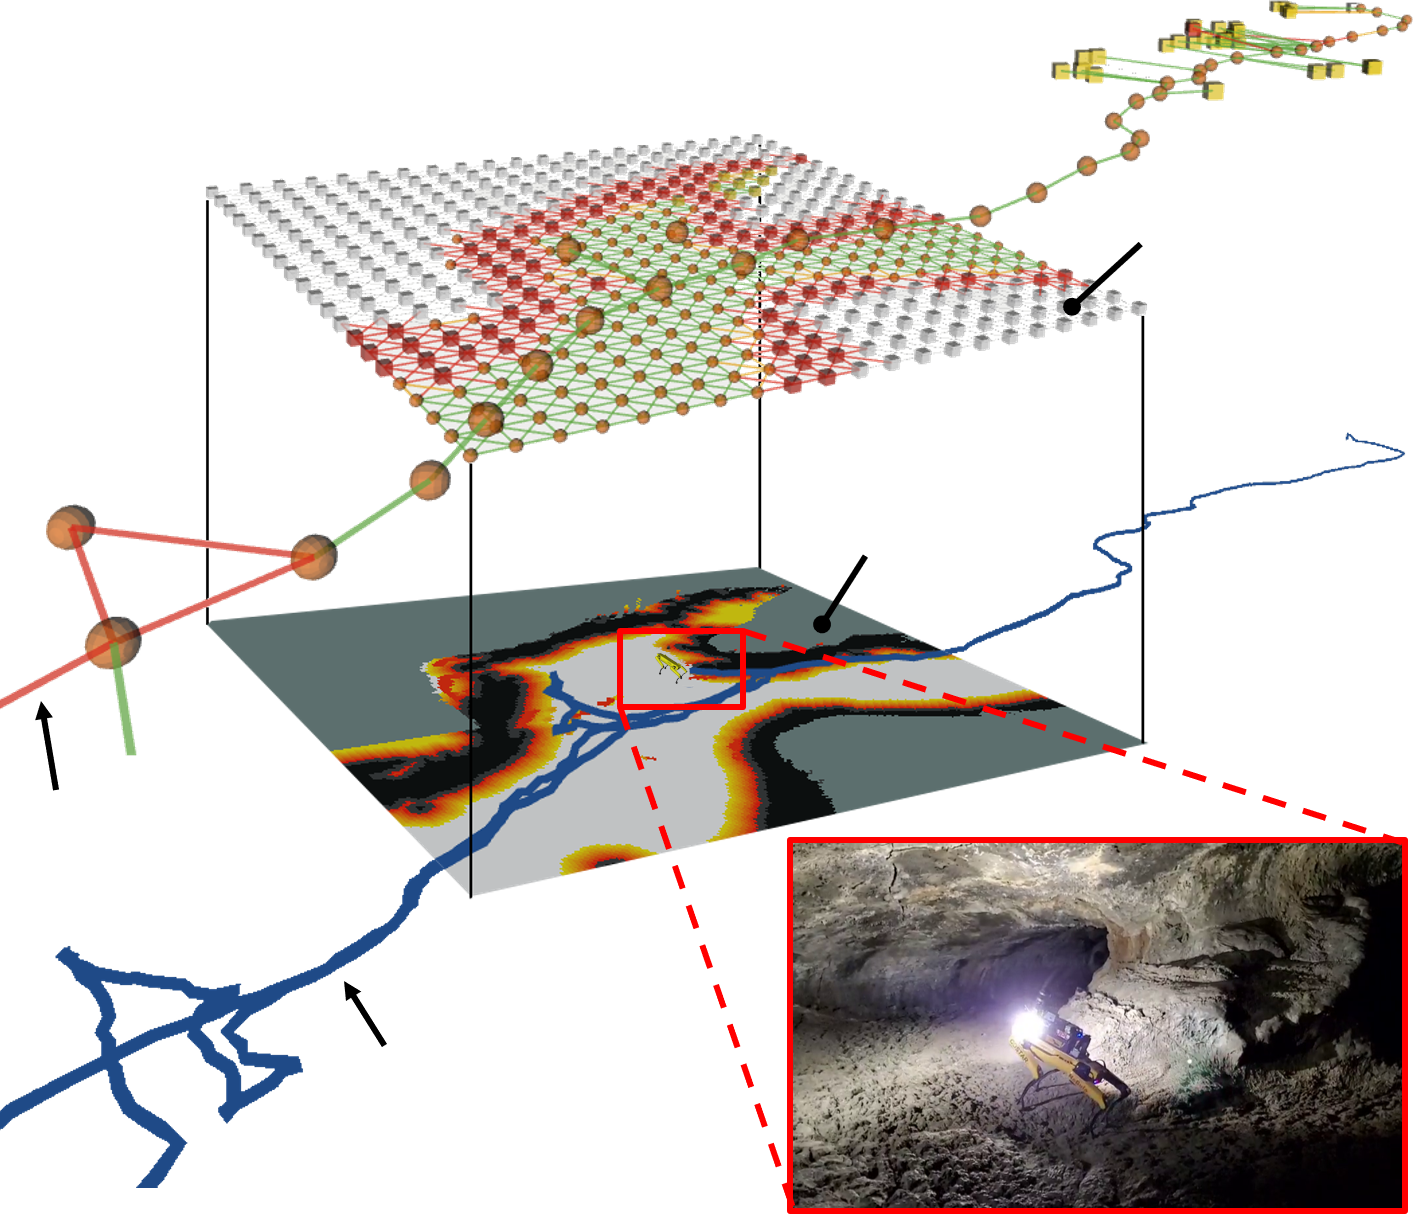
\includegraphics[width=1\columnwidth]{figures/hierarchy_labels_spot.png}};
	    \begin{scope}[x={(image.south east)},y={(image.north west)}]
	    	
	    	% Annotations 
	    	\node [font=\scriptsize,above left,align=right,black] at (0.93,0.79) {Local IRM}; %{Lattice IRM};
	    	\node [font=\scriptsize,above left,align=right,black] at (0.7,0.54) {Riskmap}; %{Graph IRM};
	    	\node [font=\scriptsize,above left,align=right,black] at (0.38,0.08) {Pose Graph};
	    	\node [font=\scriptsize,above left,align=right,black] at (0.17,0.29) {Global IRM};

	    \end{scope}
	\end{tikzpicture}	
  \caption{Hierarchical Information RoadMaps (IRMs) generated during Au-Spot's autonomous exploration of Martian-analog caves at Lava Beds National Monument, Tulelake, CA.} \label{fig:IRMs} 
\end{figure}



From a value learning perspective, a coverage planning problem in an unknown space can be considered an active learning problem over the robot's belief, where belief is defined as the probability distributions over all possible joint robot-world states.
%
The objective is to find the best action sequence that maximizes the accumulated reward over time.  The agent must accumulate data to incrementally build a model of its environment, and need to understand the effects of its actions on the quality and quantity of data it collects.

\phdone{Problem description--POMDP perspective}
Since the agent's future actions affect its belief of the world and robot state, this coverage problem is fundamentally a Partially Observable Markov Decision Process (POMDP) problem~\cite{pomdps_monahan1982}.
%A POMDP is a principled formalization of 
%a sequential decision making process under motion and sensing uncertainty.
The agent employs the underlying intrinsic model of the sequential action-observation process under uncertainty, so that it %can %(asymptotically) converge to the optimal solution in a more 
expands its search structure over the belief space and learns the value in a more sample-efficient manner than model-free learning approaches.
In addition, its non-myopic reasoning can provide better performance than frontier-based exploration approaches with one-step look-ahead.

\phdone{Gap in the state-of-the-art}
Belief value learning in the POMDP setting intrinsically suffers from the curse of dimensionality \cite{KLC98} and curse of history \cite{Pineau03}. Many powerful methods are proposed to extend the spatial and temporal horizons of POMDPs with varying degrees of efficiency and accuracy, such as \cite{silver2010monte,somani2013despot,bonet1998learning,kim2019pomhdp}. In this paper, we focus on challenging exploration problems with very large spatial extents ($>\!\!1$~km), long temporal horizons ($>\!\!1$~hour), and high dimensional belief states (including beliefs on the state of the environment) that exacerbate the curses of dimensionality and history for POMDPs. % when planning robot behaviors over the belief space.
%

% \phdone{Contributions}
% To address this problem, we introduce spatial and temporal approximations of the robot policy space to enable computational tractability while constructing a real-time online solver.
% %search space.  This decomposition allows us to approximately solve the optimization problem in a computationally tractable manner.  
% Spatially, we decompose the belief space into task-relevant partitions of the space,
% %into a robot and task-relevant graph structure 
% enriched with environment map estimates. %, which reduces our search space for good policies, 
% The partitioning structure is called an Information Roadmap (IRM) (see Fig.~\ref{fig:IRMs}). Temporally, we decompose the problem into a long-range (global) IRM which spans the entirety of the known environment, and a robot-centered short-range (local) IRM. % with fixed size. 
% We then propose a Receding Horizon Planning (RHP)-based solver to address online planning over this hierarchical POMDP structure.
% % problem in a receding horizon fashion, 
% % in real time.
% % \acomm{Consider bullet points. Link each gap to a contribution in this paragraph.}
%
%
\phdone{Contributions}
The main contribution of this work % to tackle these problems 
is in three-fold:
%
% \textit{1)} scalable belief representation of local traversability and global coverage states of the environment,
% \textit{2)} hierarchical value learning for efficient exploration policy search over a long horizon, and
% \textit{3)} field-hardened policy reconciliation technique between planning episodes for adaptive and resilient execution in the real world.
%
\vspace{-4pt}
\begin{enumerate}[label={\arabic*)}]
  \itemsep0em 
  \setlength{\itemsep}{0pt}
  \setlength{\parskip}{0pt}
\item Scalable belief representation of local traversability and global coverage states of large environments. %(Fig.~\ref{fig:IRMs}).
	\item Hierarchical value learning for efficient coverage policy search over a long horizon under uncertainty.
	% \item Field-hardened policy reconciliation technique between planning episodes for adaptive and resilient execution in the real world.
	\item Policy reconciliation between planning episodes for adaptive and resilient execution in the real world.
\end{enumerate}
\vspace{-4pt}
%
More precisely, we introduce spatial and temporal approximations of the coverage policy space to enable computational tractability for real-time online solvers.
%while constructing a real-time online solver.
%search space.  This decomposition allows us to approximately solve the optimization problem in a computationally tractable manner.  
Spatially, we decompose the belief space into task-relevant partitions of the space,
%into a robot and task-relevant graph structure 
enriched with environment map estimates. %, which reduces our search space for good policies, 
The partitioning structure is called an Information Roadmap (IRM) as shown in Fig.~\ref{fig:IRMs}.
% Temporally, we decompose the problem into a long-range (global) IRM which spans the entirety of the known explored environment, and a robot-centered short-range (local) IRM. % with fixed size. 
Temporally, we decompose the problem into local and global hierarchical levels and solve for belief space policies that provide locally near-optimal coverage plans with global completeness.
We then propose a Receding Horizon Planning (RHP)-based technique to address real-world stochasticity in state estimation and control at runtime.
%online planning over this hierarchical POMDP structure.
% problem in a receding horizon fashion, 
% in real time.
% \acomm{Consider bullet points. Link each gap to a contribution in this paragraph.}

\phdone{Outline}
The remainder of this paper is as follows: following the related work discussion, Section~\ref{sec:formulation} formalizes the unknown environment coverage problem. In Section~\ref{sec:plgrim}, we propose a hierarchical belief representation and value learning framework. Experimental results in simulation and on a physical robot are presented in Section~\ref{sec:exp_results}, and Section~\ref{sec:conclusion} concludes this paper.


%%%%%%%%%%%%%%%%%%%%%%%%%%%%%%%%%%%%%%%%%%%%%%%%%%%%%%%%%%%%%%%%%%%%%%%%%%%%%%%%
\section{Related Work}\label{sec:related_work}
\phdone{Coverage--Frontier-based exploration}
Frontier-based exploration is a widely used approach for autonomous exploration (e.g., \cite{yamauchi1997frontier,tao2007motion,keidar2012robot,heng2015efficient,gonzalez2002navigation,grabowski2003autonomous}). By continuing exploration until exhausting all remaining frontiers, frontier-based approaches can guarantee completeness of the coverage of reachable spaces.  These methods typically rely on myopic (e.g., one-step) look-ahead greedy policies, selecting the best frontier upfront. Hence they can be subject to local minima and provide suboptimal solutions in time.

\phdone{Coverage--(Model-free) RL-based approaches}
Model-free reinforcement learning (RL) has been applied to coverage and exploration problems (e.g., \cite{pathak_icm,burda2018study,rnd,ECR2018}). In this setting, the typical approach is to find a policy which maps sensor data to actions, with the objective of maximizing the reward. When it comes to long-range, large-scale, and safety-critical missions on physical robots, collecting necessary data can be a significant challenge for this class of methods.

\phdone{Coverage--(Model-based RL) POMDP approaches}
POMDP-based approaches generate a non-myopic policy by considering long-horizon action sequences (e.g., \cite{kurniawati2011motion}, \cite{bai2015intention}), interactively learning the value function, and returning the best action sequence that maximizes the accumulated rewards. Different methods have reduced the complexity of the POMDP problem in coverage and exploration problems. \citet{indelman2015planning} and \citet{martinez2009bayesian} employed a direct policy search scheme with a Gaussian belief assumption. \citet{Lauri2016planning} extended this to non-Gaussian beliefs using the POMCP (Partially Observable Monte-Carlo Planning) solver. % algorithm that uses a Monte-Carlo Tree Search \cite{silver2010monte}.
%In this work, we aim at scaling the solution even further to enable solutions for hte missions fo interste that are longer and larger than mission 
However, when it comes to the large-scale coverage missions, % discussed in Section \ref{sec:intro},
the current approaches do not scale well due to the curse of history and dimensionality \cite{Pineau03}.

\phdone{Large scale--Hierarchical approaches}
Hierarchical planning structures \cite{kaelbling2011planning} aim to tackle larger problems by employing multiple solvers running at different resolutions, and are found to be effective.  
%
In the coverage and exploration context, \citet{umari2017autonomous} applied hierarchical planning to frontier-based exploration, while  \cite{dang2019explore} extended the lower level module to a more sophisticated frontier selection algorithm which considers the information gain along each path. \citet{Lauri2016planning} replaced the lower level module with a POMDP-based planner to improve local coverage performance with non-myopic planning. \citet{kim2019bi} proposed a hierarchical online-offline solver for risk-aware navigation. \citet{vien2015hierarchical} suggested a hierarchical POMCP framework which outperformed Bayesian model-based hierarchical RL approaches in some benchmarks.


\section{Problem Formulation}
\label{sec:formulation}

Autonomous exploration in unknown environments under motion and sensing uncertainty can be formulated as a Partially Observable Markov Decision Process (POMDP), which is one of the most general models for sequential decision making.
In this section, we present a POMDP formulation for coverage problems and address its intrinsic challenges.

\subsection{Preliminaries}
\phdone{POMDP Elements}
A POMDP is described as a tuple $\langle \mathbb{S}, \mathbb{A}, \mathbb{Z}, T, O, R \rangle$, where $\mathbb{S}$ is the set of joint robot-and-world states, $\mathbb{A}$ and $\mathbb{Z}$ are the set of robot actions and observations.
At every time step, the agent performs an action $a \in \mathbb{A}$ and receives an observation $z \in \mathbb{Z}$ resulting from the robot's perceptual interaction with the environment.
% we can drop a few more words from the sentences below..
The motion model $T(s, a, s') = p(s'\,|\,s, a)$ defines the probability of being at state $s'$ after taking action $a$ at state $s$.
The observation model $O(s, a, z) = p(z\,|\,s, a)$ is the probability of receiving observation $z$ after taking action $a$ at state $s$.
The reward function $R(s, a)$ returns the expected utility for executing action $a$ at state $s$.
Belief state $b_t \in \mathbb{B}$ at time $t$ denotes a posterior distribution over states conditioned on the initial belief $b_0$ and past action-observation sequence, i.e., $b_{t} = p(s \,|\, b_0, a_{0:t-1}, z_{1:t})$.

\phdone{POMDP Objective function}
% The objective function of a generic POMDP can be described as follows.
The optimal policy of a POMDP for all time $t \in [0,\infty)$, $\pi_{0:\infty}^* \! : \mathbb{B} \to \mathbb{A}$, is defined as:
\begin{align}
  % \pi^*(b) &= \arg\max_\pi \, \mathbb{E} \sum_{t=0}^{L} \gamma^t r(b_t, \pi(b_t)),
  \pi_{0:\infty}^*(b) &= \argmax_{\pi \in \Pi_{0:\infty}} \, \mathbb{E} \sum_{t=0}^{\infty} \gamma^t r(b_t, \pi_t(b_t)),
  % \pi_{0:\infty}^*(b_0) &= \argmax_{\pi \in \Pi_{0:\infty}} \, \mathbb{E} \sum_{t=0}^{\infty} \gamma^t r(b_t, \pi(b_t)),
  % \pi_{0:\infty}^*(\cdot) &= \argmax_{\pi \in \Pi_{0:\infty}} \, \mathbb{E} \sum_{t=0}^{\infty} \gamma^t r(b_t, \pi(b_t)),
  \label{eq:objective_function}
\end{align}
where $\gamma \in (0, 1]$ is a discount factor for the future rewards, $\Pi_{0:\infty}$ is the space of possible policies, and $r(b,a)=\int_s R(s,a)b(s)\mathrm{d}s$ denotes a belief reward which is the expected reward of taking action $a$ at belief $b$. %\acomm{Ali says define $\pi$, but $\pi$ is just sampled from space of all policies$\Pi_{0:\infty}$?}

% \subsection{Unknown Environment Coverage Problem Formulation}
\subsection{Unknown Environment Coverage Problems}

\phdone{Coverage Problem}
For our coverage planning problem, we define the state as $s = (q, W)$, where $q$ is the robot state and $W$ is the world state. We maintain two representations of the world, i.e., $W = (W_{r}, W_{c})$, where $W_{r}$ denotes the world traversal risk state and $W_{c}$ is the world coverage state.

$W_{r}$ encodes the traversability risk of the world with respect to a robot's dynamic constraints. This state is critical in capturing traversability-stressing elements of the environment (slopes, rough terrain, and narrow passages, etc.) and is typically constructed by aggregating long-range sensor measurements. %$W_{r}$ provides an estimation of the trajectory (i.e., path length and probability of failure), associated with a motion control. 
% For any given trajectory (or action $a$ along the trajectory), 
% we can query $W_{r}$ for the risk of following the trajctory (probability of failure).
The cost function $C(W_{r}, q, a)$ returns the actuation effort and risk associated with executing action $a$ at robot state $q$ on $W_{r}$.
% by capturing the stability of a robot as it negotiates terrain (e.g., slopes, rough terrain, low traction areas, narrow passages, etc) 

$W_{c}$ provides an estimation of what parts of the world have been observed, or \textit{covered}, by a particular sensor.
The coverage state is generated by specific sensor measurements, which may not necessarily be useful as navigational feedback, but instead are based on a task at hand. For instance, the coverage sensor may be a thermal camera for detecting thermal signatures, or a vision-based camera for identifying visual clues in the environment. 
As a robot moves, the sensor footprint sweeps the environment, expanding the covered area, or more generally, the task-relevant information about the world.
% For any given trajectory (or action $a$ along the trajectory), function $I(W_{c}, a)$ returns the information gain, or accumulated covered area, by taking action $a$ at robot state $q$ on $W_{c}$.
% By incorporating a sensor field-of-view $F:V\rightarrow \mathcal{P}(V)$, which maps each node to a subset of "viewable" nodes, and adding the objective of minimizing travel distance, the coverage problem can be seen as a generalization of the traveling salesman problem -- the \emph{covering salesman problem} (CSP).  In the CSP, the objective is to determine the minimum length path through a subset of nodes $\{v_i\}_i \subseteq V_{free}$ such that every free node is within the accumulated sensor field-of-view: $V_{free} \subseteq \cup_i F(v_i)$.
% maintain two multi-range representations of the world (risk, coverage)  

% \ph{Action Reward} 
The coverage planning objective is to determine a trajectory through an environment that maximizes information gain $I$ while simultaneously minimizing action cost $C$. As such, the traversal risk and coverage states form the basis of the coverage reward function:
\begin{align}
  % R(s, a) = f(I(z(s, a), W_{c}),\; C(q, a, W_{r})),
  % R(s, a) = f(I(W_{c}, z),\; C(W_{r}, q, a)),
  % R(s, a) = \mathrm{fn}(I(W_{c}, z),\; C(W_{r}, q, a)),
%   R(s, a) = \mathrm{fn}(I(W_{c}, a),\; C(W_{r}, q, a)),
  R(s, a) = f(I(W_{c}, a),\; C(W_{r}, q, a)),
  \label{eq:coverage_reward}
\end{align}
where $I(W_{c}, a) = H(W_{c}) - H(W_{c} \,|\, a)$ is quantified as reduction of the entropy $H$ in $W_{c}$ after taking action $a$. 
%
%Henceforth, we use \textit{observed} to denote long-range/environmental sensor gathering for $W_r$ encoding, while we use \textit{covered} to denote short-range/data-collection/perception sensor gathering for $W_c$ encoding.
%
\phdone{Receding Horizon Planning}
Note that in unknown space coverage domains, we do not have strong priors about the parts of the world that have not yet been observed. Hence, knowledge about $W_{c}$ and $W_{r}$ in Eq.~(\ref{eq:coverage_reward}) at runtime is incomplete and often inaccurate.
% By plugging Eq.~(\ref{eq:coverage_reward}) into Eq.~(\ref{eq:objective_function}), we can formulate the coverage planning problem with an infinite planning horizon in a POMDP setting.
% Then we can identify several fundamental challenges to solve this problem.
%
% Thus, it is fundamentally not feasible to solve an unknown environment coverage problem when formulated as in Eq.~(\ref{eq:objective_function}) for an infinite horizon.
% Instead, Receding Horizon Planning (RHP) scheme has been widely adopted in most of the state-of-the-art in this domain \cite{bircher2016receding}.
Thus, in such domains, a Receding Horizon Planning (RHP) scheme has been widely adopted as the state-of-the-art \cite{bircher2016receding}.

\phdone{RHP Objective Function}
In POMDP formulation with RHP, the objective function in Eq.~(\ref{eq:objective_function}) is modified:
\begin{align}
  \pi_{t:t+T}^*(b) &= \argmax_{\pi \in \Pi_{t:t+T}} \, \mathbb{E} \sum_{t'=t}^{t+T} \gamma^{t'-t} r(b_{t'}, \pi_{t'}(b_{t'})),
  \label{eq:receding_objective_function}
\end{align}
where $T$ is a finite planning horizon for a planning episode at time $t$.
Given the policy from the last planning episode, only a part of the optimal policy, $\pi^*_{t:t+\Delta t}$ for $\Delta t \in (0, T]$, will be executed at runtime. A new planning episode will start at time $t+\Delta t$ with updated belief about $q$, $W_{c}$, and $W_{r}$.



\subsection{Challenges} \label{ssec:challenges}
% Solving the POMDP-RHP coverage problem in Eq.~(\ref{eq:receding_objective_function}) necessitates balancing conflicting planner requirements: long time horizons and high resolution action spaces, as well as consistency and resiliency between successive plans.

% Environment:
% - Unknown 
%     - Reliance on noise-susceptible belief 
%     - Receding-horizon introduces consistency vs. resiliency trade-off:
%         - Path consistency between episodes
%         - Path resilience to inaccurate information
    
% - Large
%     - Memory efficient world representation (computationally constrained)

% - Difficult Terrain
%     - precision --> high resolution action sequence (computationally constrained)
%     - myopic could be risky? not really

% Objective:
% - Coverage
%     - efficiency --> long horizon action sequence (computationally constrained)
 
%  The agent must understand how its actions affect the coverage belief state. 
   
% We detail the challenges with solving the coverage planning problem with a receding horizon, Eq.~(\ref{eq:receding_objective_function}), for an unknown, large ($>\!\!1$~km), and rugged-terrain environment over long-time scales ($>\!\!1$~hour).
We broadly identify the challenges associated with solving the unknown coverage planning problem, Eq.~(\ref{eq:receding_objective_function}), as computational complexity---in both time and space---and conflicting policy objectives over consecutive planning episodes, arising from unexpected updates in the belief at runtime.


% \vspace{-2.5pt}
\subsubsection{Time Complexity:} \hfill
\vspace{-0.25pt}


% POMDP planning suffers from \textit{curse of dimensionality} \cite{KLC98} and \textit{curse of history} \cite{Pineau03}. The former difficulty refers to the fact that "dimensionality" of the belief space is equal to "cardinality" (size) of the underlying state space. %, and the the computational complexity of a belief update is quadratic in the size of the state space: $\mathcal{O}(|\mathbb{S}|^2)$. 
% The latter difficulty refers to the fact that the computational complexity of evaluating possible action-observation combinations grows exponentially in planning depth $d$, $\mathcal{O}(|\mathbb{A}|^d|O|^d)$. Together, both \textit{curses} result in a POMDP planning complexity of $\mathcal{O}((|\mathbb{A}||O|)^d|\mathbb{S}|^2)$. Hence, a crudely defined belief- and action-space approximations can likely result in a very long planning time, untenable for a real-time system that must react quickly to new sensor information. An agent's onboard computational resources upper bound the planner's computational complexity.
% 
% The former difficulty is sourced in the fact that the state space grows exponentially with the number of state variables, and the latter difficulty refers to the fact that the time complexity of evaluating possible action-observation combinations grows exponentially with planning depth $d$; $\mathcal{O}(|\mathbb{A}|^d|\mathbb{Z}|^d)$.

\noindent
POMDP planning suffers from \textit{the curse of dimensionality} \cite{KLC98} and \textit{the curse of history} \cite{Pineau03}. The former difficulty refers to fact that size of the belief grows exponentially with the size of the underlying state space. The latter difficulty refers to the fact that the number of action-observation sequences grows exponentially with the planning depth $d$, i.e., $\mathcal{O}(|\mathbb{A}|^d|\mathbb{Z}|^d)$.
% The former difficulty is sourced in the fact that the state space grows exponentially with the number of state variables, and the the time complexity of belief update is quadratic in the size of the state space; $\mathcal{O}(|\mathbb{S}|^2)$.
% The latter difficulty refers to the fact that the time complexity of evaluating possible action-observation combinations grows exponentially with planning depth $d$; $\mathcal{O}(|\mathbb{A}|^d|\mathbb{Z}|^d)$.
% Together, the above two \textit{curses} result in a POMDP planning complexity of $\mathcal{O}(|\mathbb{A}|^d|\mathbb{Z}|^d|\mathbb{S}|^2)$.
% ORIGINAL TEXT ABOVE WAS ALSO GOOD IF WE HAVE SOME SPACE!
% More specifically, the time complexity of POMDP planning is $\mathcal{O}(|\mathbb{S}|^2(|\mathbb{A}||\mathbb{Z}|)^d)$,
% where $\mathcal{O}(|\mathbb{S}|^2)$ is due to the belief update, and  $\mathcal{O}((|\mathbb{A}||\mathbb{Z}|)^d)$ is from the evaluation of possible action-observation sequences up to planning depth $d$.
% More specifically, the time complexity of POMDP planning is $\mathcal{O}((|\mathbb{A}||\mathbb{Z}|)^d)$
% to evaluate possible action-observation sequences up to planning depth $d$.
% The 
% % POMDP planning suffers from \textit{the curse of dimensionality} \cite{KLC98} and \textit{the curse of history} \cite{Pineau03},
% referring to the exponential complexity in the number of states and the planning horizon, respectively.
% The former difficulty is sourced in the fact that the state space grows exponentially with the number of state variables, and the the time complexity of belief update is quadratic in the size of the state space; $\mathcal{O}(|\mathbb{S}|^2)$.
% The latter difficulty refers to the fact that the time complexity of evaluating possible action-observation combinations grows exponentially with planning depth $d$; $\mathcal{O}(|\mathbb{A}|^d|\mathbb{Z}|^d)$.
% Together, the above two \textit{curses} result in a POMDP planning complexity of $\mathcal{O}(|\mathbb{A}|^d|\mathbb{Z}|^d|\mathbb{S}|^2)$.
% ORIGINAL TEXT ABOVE WAS ALSO GOOD IF WE HAVE SOME SPACE!
% More specifically, the time complexity of POMDP planning is $\mathcal{O}(|\mathbb{S}|^2(|\mathbb{A}||\mathbb{Z}|)^d)$,
% where $\mathcal{O}(|\mathbb{S}|^2)$ is due to the belief update, and  $\mathcal{O}((|\mathbb{A}||\mathbb{Z}|)^d)$ is from the evaluation of possible action-observation sequences up to planning depth $d$.
% More specifically, the time complexity of POMDP planning is $\mathcal{O}((|\mathbb{A}||\mathbb{Z}|)^d)$
% to evaluate possible action-observation sequences up to planning depth $d$.
% As a representative scenario considered in this work, 
As an example, for large-scale exploration of a 1~km-long environment with an action resolution of 1~m, 
% 1~m traverse per action by the agent
the planning depth $d$ must be at least $10^3$ in order to reason about the coverage plan across the environment.
%Hence, the POMDP time complexity makes it computationally intractable to find a solution without adequate approximation of the policy space and effective policy search algorithms.

% $|S|$

% $dim(B) = |S|$

% $m^{|S|}$

% $m^{|S|} \sim = beliefParamVector$

% $m^{|Q|\times|\mathbb{W}|}$

% $m^{|Q|\times|n|^k}$

% $m^{|\mathbb{W}|}$

% $|\mathbb{W}|\times beliefParameter$

% $\mathcal{O}(|\mathbb{A}|^d|\mathbb{Z}|^d|\mathbb{S}|^2)$
% $\mathcal{O}(|\mathbb{A}|^d|\mathbb{Z}|^d (|n|^k\times |levels|)^2)$


% \vspace{-2.5pt}
\subsubsection{Space Complexity:} \hfill
\vspace{-0.25pt}

\noindent
In addition to the classic time complexity of POMDPs, space complexity also poses a considerable challenge when handling the unknown environment coverage problem.
% In unknown environment exploration problems, the POMDP solver's space complexity is dominated by the world state representation.
% Recall that state $s = (q, W)$ in the coverage problem includes $W$ since the world is only partially observable, and the coverage state $W_c$ changes as the agent explores.
% Primary factors affecting this complexity are the environment size, spatial resolution, number of state variables, and the fidelity of the values assigned to these variables (e.g., Boolean vs. floating-point).
Since $s = (q, W)$, the space complexity is dominated by the world state $W$. 
% , where $O(W)=\mathcal{O}(|n|^k)$
% Since the state $s = (q, W)$ in the coverage problem contains $W$, the space complexity is dominated by the world state representation.
%, such as the environment size, spatial resolution, and the fidelity of state variables (e.g., Boolean vs. floating-point).  %% THIS SENTENCE CAN BE OMITTED IF NEEDED!
% The space complexity of representing the world state is $\mathcal{O}(|n|^k)$, where $n$ denotes the number of elements in the discretization and $k$ is the number of state variables describing each element. 
% is the number of spatial elements composing the representation and $k$ is the 
% number of state variables describing each element.
%
%
% For example, a grid structure with 1~m resolution requires 8~MB of memory to represent a single snapshot of 1$\times$1~km environment if each grid cell stores risk and coverage states as floating-point variables.
% For example, a grid structure with 1~m resolution requires 8~MB of memory to represent a single snapshot of a 1~km$^2$-size world state with floating-point risk and coverage values associated with each cell.
For example, in a grid world, the memory complexity is $\mathcal{O}(|n|^k)$, with $n$ and $k$ denoting the number of discretization levels and the grid dimension, respectively. For a 1~km$^2$ environment at a 0.1~m resolution, %(for high-fidelity motion planning), 
with floating-point risk and coverage values stored in every cell, required memory is 800~MB. This amount of memory should be allocated for every search node, and thus the full space complexity of planning is $\mathcal{O}(|\mathbb{A}|^d |\mathbb{Z}|^d |n|^k)$ during each planning episode.

% Then the space complexity of a POMDP planning is $\mathcal{O}(|\mathbb{A}|^d |\mathbb{Z}|^d |n|^k)$ during a single planning episode.
%
% For example, assuming use of a grid structure, the memory required to represent a single snapshot of a 1~km$^2$ environment at a 1~m resolution, with floating-point risk and coverage values stored in every cell, is 8~MB.
% of memory to represent a single snapshot of a 1~km$^2$-size world state with floating-point risk and coverage values associated with each cell.
% Since a POMDP solver must allocate memory for the storage of $(|\mathbb{A}||\mathbb{Z}|)^d$ number of world states during a single planning episode, this crude world representation
% Since the space complexity of a POMDP solver is $\mathcal{O}(|\mathbb{A}|^d |\mathbb{Z}|^d |n|^k)$ during a single planning episode, this crude world representation
% (in the order of magnitude of $(|\mathbb{A}||\mathbb{Z}|)^d$),
% is untenable for a real-time system.
% The space complexity of a POMDP planning is $\mathcal{O}(|\mathbb{A}|^d |\mathbb{Z}|^d |n|^k)$ during a single planning episode.
% Thus, an efficient method of representing the world state is required.
% this space complexity gets untenable, especially for onboard computing systems, and necessitates an efficient way of representing the world state.

% $|\mathbb{S}| = |\mathbb{Q}|\times|\mathbb{W}|$

% $|\mathbb{W}| = |n|^k \times |levels|$

% $\mathcal{O}(|n|^k\times |levels| \times copyComplexity)$


% \vspace{-2.5pt}
% \subsubsection{Policy Concatenation} \hfill
% \subsubsection{Policy Reconciliation:} \hfill
\subsubsection{Unexpected Belief Updates:} \hfill
% \subsubsection{Unexpected Updates in Beliefs:} \hfill
\vspace{-0.25pt}

\noindent
% As the robot explores its environment, it receives new sensory information, updates its belief, and constructs a new coverage policy in a receding horizon fashion.
% Policies generated during consecutive planning episodes need to achieve  \textit{consistency} and \textit{resiliency}. Consistency refers to respecting robot's kinodynamic constraints by ensuring smooth trajectories and continuous velocities during transitions from one policy to the next. Resiliency refers to the ability to adapt to unexpected hazards by quickly reacting to changes in world risk map $W_r$ and avoiding collisions.
% Thus, it is desired to find a balance between these two typically conflicting requirements, particularly for safety-critical systems.
% 
% Plan consistency and resiliency are often in opposition.
% Unexpected changes in the local world representation, due to sensor data delays or map prediction errors, may require aggressive maneuvers to avoid a collision. However, if the maneuver violates a robot's motion constraints (e.g., minimum turning radius), then the robot may destabilize and become inoperable. Thus, it is vital to find a balance between plan consistency and resiliency, particularly for safety-critical systems.
% operating in natural disaster areas, is vital so that a coverage mission does not end prematurely due to physical robot failure. 
As the robot explores its environment, it receives new sensory information, updates its belief, and constructs a new coverage policy in a receding horizon fashion.
Policies generated during consecutive planning episodes must respect the kinodynamic constraints of the robot, while simultaneously adapting to unexpected hazards in the environment.
We refer to these two distinct, and often opposed, objectives as \textit{consistency} and \textit{resiliency} of the receding-horizon policy, respectively.
% Consistency between consecutive policies is generally preferred so that the robotic system maintains a smooth trajectory free of extreme velocity fluctuations.
Path consistency ensures smooth trajectories and continuous velocities during transitions from one policy to the next, while path resiliency ensures the path adapts to unexpected changes in the world risk state. %$W_r$.
% in order to avoid collisions.
% However, if there are unexpected changes to the robot's understanding of $W_r$, the robot must update its motion through a resilient and adaptive policy to avoid a collision.
Thus, it is imperative to find a balance between policy consistency and resiliency, particularly for safety-critical systems.
% Plan consistency and resiliency are often in opposition.
% Unexpected changes in the local world representation, due to sensor data delays or map prediction errors, may require aggressive maneuvers to avoid a collision. However, if the maneuver violates a robot's motion constraints (e.g., minimum turning radius), then the robot may destabilize and become inoperable. Thus, it is vital to find a balance between plan consistency and resiliency, particularly for safety-critical systems.
% %operating in natural disaster areas, is vital so that a coverage mission does not end prematurely due to physical robot failure. 




% ==============================

% % \vspace{-2.5pt}
% \subsubsection{Computational Complexity:} \hfill
% \vspace{-0.25pt}

% \noindent
% POMDP planning suffers from \textit{curse of dimensionality} \cite{KLC98} and \textit{curse of history} \cite{Pineau03}. The former difficulty refers to the fact that "dimensionality" of the belief space is equal to "cardinality" (size) of the underlying state space. %, and the the computational complexity of a belief update is quadratic in the size of the state space: $\mathcal{O}(|\mathbb{S}|^2)$. 
% The latter difficulty refers to the fact that the computational complexity of evaluating possible action-observation combinations grows exponentially in planning depth $d$, $\mathcal{O}(|\mathbb{A}|^d|O|^d)$. Together, both \textit{curses} result in a POMDP planning complexity of $\mathcal{O}((|\mathbb{A}||O|)^d|\mathbb{S}|^2)$. Hence, a crudely defined belief- and action-space approximations can likely result in a very long planning time, untenable for a real-time system that must react quickly to new sensor information. An agent's onboard computational resources upper bound the planner's computational complexity.
% % As a concrete example, finding the coverage path spanning $1~hr$ through a $1 km$ environment with precise motions that can negotiate rugged terrain ($1~m$ actions into the $8$ direction combined cardinal and intercardinal directions), and an observation space spanning the environment containing both the world coverage an risk state ($1000^2$), the time complexity is $\mathcal{O}((|8||1000^2|)^{1000})$ (probably wrong), assuming no belief update.

% % \vspace{-2.5pt}
% \subsubsection{Space Complexity:} \hfill
% \vspace{-0.25pt}

% \noindent
% \acomm{When it comes to "unknown" environment exploration, the curse of dimensionality is severely exacerbated, as it in this case the state space $\mathbb{S}=\mathbb{Q}\times\mathbb{W}$,} and the POMDP planner's space complexity is dominated by the world state representation. Primary factors affecting this complexity are the environment size, spatial resolution, number of state variables, and the fidelity of the values assigned to these variables (e.g. Boolean vs. floating-point). Accordingly, the planner's space complexity is $\mathcal{O}(|n|^k)$, where $n$ is the map size \textcolor{blue}{(map is too specific)} and $k$ is the number of state variables. As a concrete example, assuming use of a grid structure, the memory required to represent a $1~km$ environment at a $0.1~m$ resolution, where each map cell stores risk and coverage probabilities as a floating-point variable, is $4$ MB---an impractical allocation for an onboard system. Thus, as was the case with time complexity, an agent's onboard computational resources upper bound the planner's space complexity, particularly relating to the world state representation.

% % \subsubsection{Policy Concatenation} \hfill
% % \vspace{-2.5pt}
% \subsubsection{Policy Reconciliation:} \hfill
% \vspace{-0.25pt}

% \noindent
% As the agent explores its environment, it receives new sensor information and updates its plan accordingly in a receding horizon fashion. %This continuous acquisition of new information, in conjunction with the computational constraints imposed by a real-time system, means that the agent can only construct a finite horizon optimal policy during a single planning episode. 
% Policies generated during consecutive planning episodes must respect the dynamic constraints of the robot (consistency), while simultaneously adapting to unexpected hazards in the environment (resiliency). Plan consistency and resiliency are often in opposition. Unexpected changes in the local world representation, due to sensor data delays or map prediction errors, may require aggressive maneuvers to avoid a collision. However, if the maneuver violates a robot's motion constraints (e.g., minimum turning radius), then the robot may destabilize and become inoperable. Thus, it is vital to find a balance between plan consistency and resiliency, particularly for safety-critical systems.
% %operating in natural disaster areas, is vital so that a coverage mission does not end prematurely due to physical robot failure. 

% ==============================



% % = (1000/.1)^2*4

% POMDP complexity -> relationship between factors (horizon, branching factors-action space, observation space-belief space resolution)
% O((|action| * |observation|)^depth)

% **Constraints (computational-time complexity, memory-space complexity) --> CLARIFICATION WITH OTHER PEOPLE (Kyon?)
% --> Curse of dimensionality/history

% Our case:
% * Time complexity
% Space > 1km
% action (motion) resolution ~ 1m  *with the help of local motion planner
% action set: 8-neighbor (orientation?)
% observation: Gaussian-type? 0/1 FOV-sensor model? --> Combination of obstacle cells in FOV: O(2^(5x5)) for FOV 5m --> (Relevant to Memory)
% Depth ~ 1000 steps
% --> O((8*1000)^1000) --> blows up!


% % A* algorithm
% % 100x100 cells --> how much of cells should be memorized at a time (space complexity)

% * Memory --> per O(1) each operation % (not very tightly related to algorithm's space complexity)
% Representation of W_r, W_c

% General:
% risk % (traversability) (--> edge connection)
% Coverage % (IG) (--> Frontier)

% Our case:
% Real-time system constraint?

% 0.1m resolution costmap
% 1km for this resolution
% (1e5)^2 in 2D representation
% 1 cell in double-type --> 4byte? --> ?GB x2 (r, c) --> blows up!




% We detail the challenges associated with solving the coverage planning problem in an unknown, large (> 1 km), and rugged-terrain environment over long-time scales (> 1 hr) using a POMDP-RHP formulation. We categorize these challenges as...

% Hierarchical (1), Roadmap (2)
% - Curse of Dimensionality: in partially observable environment, agent must reason in space of beliefs (probability distributions over states). If agent naively discretizes belief space, the number of discrete beliefs then grows exponentially with the number of states.
%     - Large Environment
%     - Rugged-terrain

% POMDP Solver (3)
% - Curse of History: number of action-observation histories grows exponentially with the planning horizon.
%     - Globally: Large environment, Long time scales
%     - Locally: High resolution state space

% Hierarchical (1), Roadmap (2)
% - Memory Efficient Representation
%     - Large Environment
%     - Rugged-terrain
%     - Long time scales

% safety-critical RH implementation (4)
% - Receding Horizon: incomplete information / how to deal with updating belief
%     - Consistency between episodes --> path concatenation assuming belief is accurate
%     - Resilience to noise
    
    
    
    
% Smart discretization of belief space

% - long time horizons (> 1 hour)
% - large spatial extents (> 1 km)
% - high dimensional belief states

% Objective: Coverage 
% - Efficiency --> long horizon action sequence

% Environment attribute: Unknown 
% What's difference between belief and RH in terms of motivation?
% - Incomplete information --> Receding Horizon Implementation 
%     - Consistency between episodes --> path concatenation assuming belief is accurate
%     - But what if belief is not accurate? This leads to resilience
% - Belief --> noise susceptible --> Bad information
%     - Resilience to noise
    
% Environment attribute: Large 
% - Memory efficient representation
% - Long horizon

% Environment attribute: Rugged-Terrain 
% - High resolution action sequence


% Efficient exploration of a large-scale environment with complex terrain requires reasoning over long temporal horizons while maintaining the ability to locally plan precise motions that can negotiate complex terrains. These two requirements---optimal action sequences spanning the known environment and high resolution action spaces---are incompatible given a robot's limited onboard computational resources during real-time planning. Therefore, the solver and action space must be designed with this resource-constraint (conflict) in mind. Furthermore, limited computational resources also necessitate a memory-efficient world representation that stores high-fidelity information about the entire known environment, which can be queried when solving for the long-horizon coverage policy. 



%%%%%%%%%%%%%%%%%%%%%%%%%%%%%%%%%%%%%%%%%%%%%%%%%%%%%%%%%%%%%%%%%%%%%%%%%%%%%%%%
\section{PLGRIM: Hierarchical Coverage Planning on Information Roadmaps}
\label{sec:plgrim}

\phdone{Framework Overview}
In this section, we present a novel and field-hardened coverage planning autonomy framework, \textit{PLGRIM (Probabilistic Local and Global Reasoning on Information roadMaps)}, for exploration of large-scale unknown environments with complex terrain.
% Our key ideas to tackle the challenges described in Section~\ref{ssec:challenges} are as follows:
Our proposed methods to tackle the challenges described in Section~\ref{ssec:challenges} are:
% Our key ideas to tackle the challenges in Section~\ref{ssec:challenges} are:
% To handle the \textit{Planner Horizon vs. Resolution} tradeoff:
% This reduces the blah blah complexity by doing blah
%
\vspace{-4pt}
\begin{enumerate}[label={\arabic*)}]
  \itemsep0em 
  \setlength{\itemsep}{0pt}
  \setlength{\parskip}{0pt}
  \item \label{en:idea1} Space Complexity:
  We introduce a hierarchical belief space representation that is compact, versatile, and scalable.
  We refer to this representation as an Information RoadMap (IRM).
  Hierarchical IRMs can effectively encode a large-scale world state, while simultaneously capturing high-fidelity information locally.
%   The hierarchical IRMs can effectively encode the large-scale world states, while capturing the high-fidelity local information.
  \item \label{en:idea2} Time Complexity:
  We propose hierarchical POMDP solvers that reason over long horizons within a suitable replanning time with locally near-optimal performance. Higher-level policies guide lower-level policies, resulting in a cascaded decision process.
  \item \label{en:idea4} Unexpected Belief Updates:
  We introduce a receding-horizon policy reconciliation method that respects the robot's dynamic constraints while ensuring resiliency to unexpected observations.
\end{enumerate}
\vspace{-1pt}

% \noindent Finally, we extend the Receding Horizon Planning (RHP) scheme to provide consistent and resilient coverage planning for safety-critical systems (\textit{Plan Consistency vs. Resiliency} tradeoff).

% \begin{enumerate}[label={\arabic*)}]
%   \item We extend the Receding Horizon Planning (RHP) scheme to provide consistent and resilient coverage planning for safety-critical systems (Challenge~\ref{en:issue3a} and \ref{en:issue3b}).
% \end{enumerate}
% \textcolor{blue}{(proposal #1 is general contribution, so it covers all challenges?)} Proposals~(1), (2)~address the \textit{Time Complexity} challenge, proposal~(3)~addresses the \textit{Space Complexity} challenge, and proposal~(4)~addresses the \textit{Policy Concatenation} challenge. 
\noindent
In the following subsections, we provide the technical details about the proposed framework, illustrated in Fig.~\ref{fig:framework}. 

% (subsections)
% 4.1. Hierarchical Belief Space Representation -- Compact world representation (IRM): 1.b
% 4.2. Hierarchical Coverage Policy Formulation -- Hierarchical world representation and planning structure: 2.a, (1.b)
% 4.3. Efficient/Real-time (Hierarchical) POMDP solvers --  Efficient POMDP solver (QMDP, POMCP): 2.b
% 4.4. Consistent and resilient planning (RHP formulation + adaptation): 3.a-b


% \subsection{Hierarchical POMDP Policy Formulation}
% \subsection{POMDP Problem Decomposition}
\label{ssec:hierarchical_policy}

% \begin{figure}[t!]
% \centering
%     \begin{tikzpicture}
%     \node[anchor=south west,inner sep=0] (image) at (0,0) {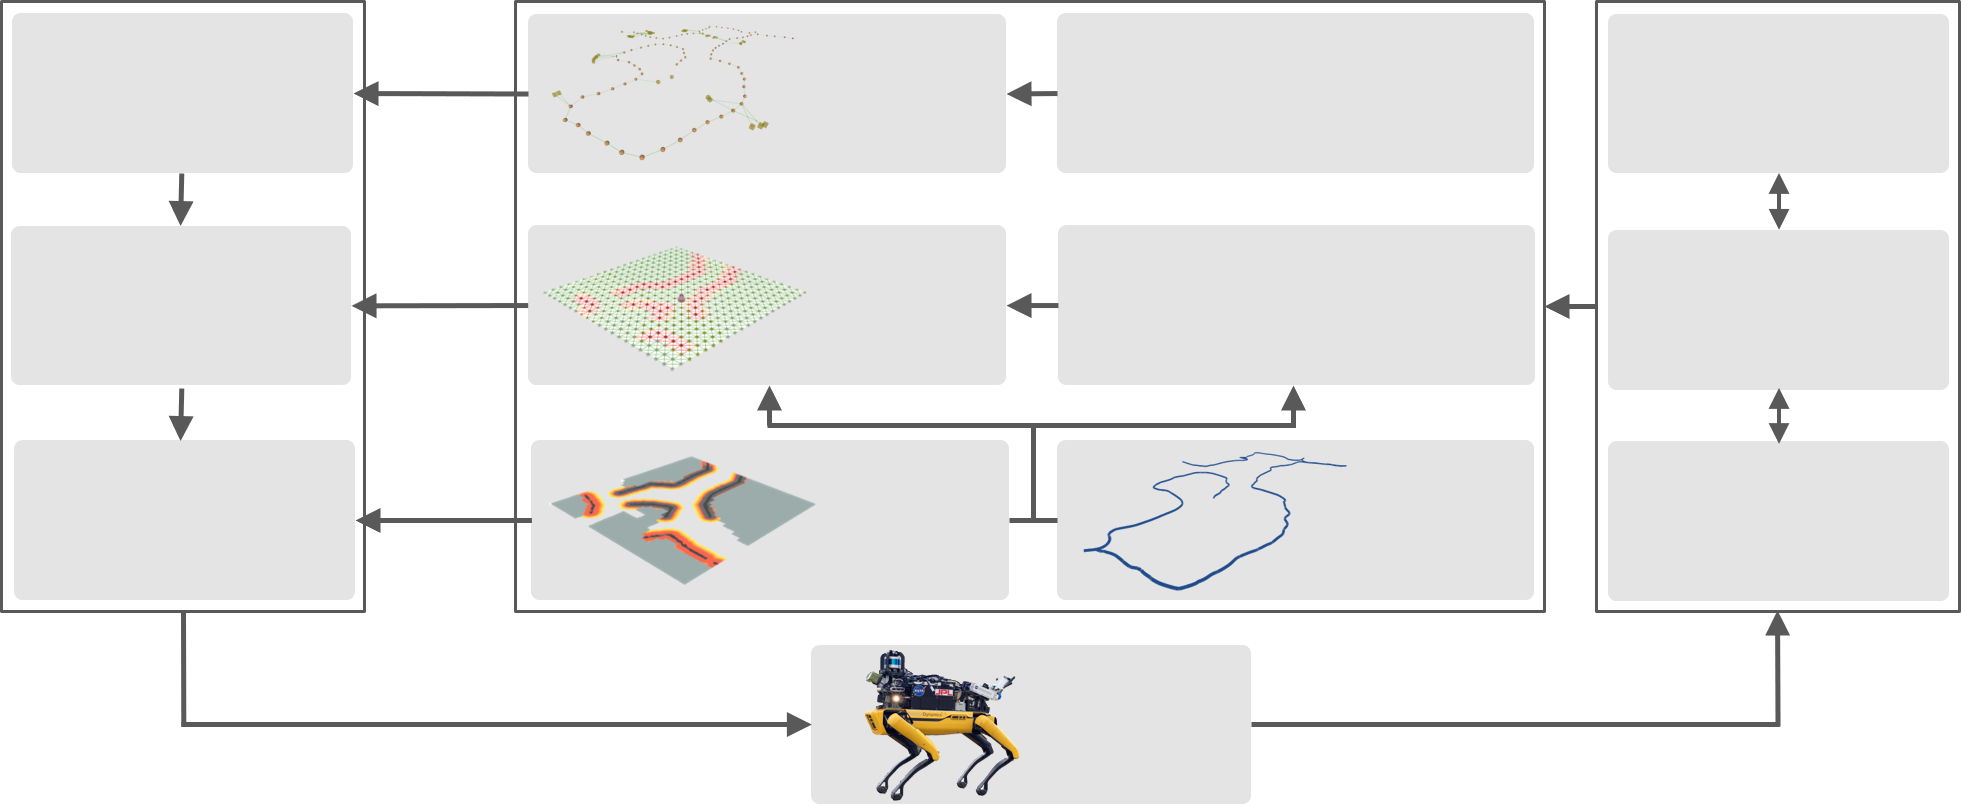
\includegraphics[width=1\columnwidth]{figures/diagram_v16.png}};
% 	    \begin{scope}[x={(image.south east)},y={(image.north west)}]
% 	    	
% 	    	% Annotations 
% 	    	\node [font=\tiny,above left,align=right,black] at (0.265,0.61) {Local};
% 	    	\node [font=\tiny,above left,align=right,black] at (0.264,0.53) {IRM};
% 	    	\node [font=\tiny,above left,align=right,black] at (0.275,0.87) {Global}; 
% 	    	\node [font=\tiny,above left,align=right,black] at (0.264,0.79) {IRM}; 
% 	    	\node [font=\tiny,above left,align=right,black] at (0.265,0.255) {Risk\\Map}; 
% 	    	
% 	    	\node [font=\scriptsize,above left,align=right,black] at (0.99,0.54) {Odometry}; 
% 	    	\node [font=\scriptsize,above left,align=right,black] at (1,0.81) {3D Mapping}; 
% 	    	\node [font=\scriptsize,above left,align=right,black] at (1,0.28) {Traversability}; 	
% 	    	
% 	    	\node [font=\scriptsize,above left,align=right,black] at (0.76,0.59) {Path Traversal}; 
% 	    	\node [font=\scriptsize,above left,align=right,black] at (0.73,0.52) {Checker}; 
% 	    	\node [font=\scriptsize,above left,align=right,black] at (0.72,0.86) {Frontier}; 
% 	    	\node [font=\scriptsize,above left,align=right,black] at (0.73,0.77) {Manager}; 
% 	    	\node [font=\scriptsize,above left,align=right,black] at (0.77,0.33) {Pose}; 
% 	    	\node [font=\scriptsize,above left,align=right,black] at (0.78,0.25) {Graph}; 
% 	    	
% 	    	\node [font=\tiny,above left,align=right,black] at (0.52,0.85) {Global IRM}; 
% 	    	\node [font=\tiny,above left,align=right,black] at (0.51,0.78) {Manager}; 
% 	    	\node [font=\tiny,above left,align=right,black] at (0.52,0.59) {Local IRM}; 
% 	    	\node [font=\tiny,above left,align=right,black] at (0.51,0.51) {Manager}; 
% 	    	\node [font=\scriptsize,above left,align=right,black] at (0.508,0.33) {Risk}; 
% 	    	\node [font=\scriptsize,above left,align=right,black] at (0.51,0.25) {Map}; 
% 	    	
% 	    	\node [font=\scriptsize,above left,align=right,black] at (0.38,0.08) {Velocity Commands};
% 	    	\node [font=\scriptsize,above left,align=right,black] at (0.85,0.08) {Sensor Data};
% 	    	\node [font=\scriptsize,above left,align=right,black] at (0.63,0.05) {Robot};
% 	    	
% 	    	\node [font=\tiny,above left,align=right,black] at (0.193,0.85) {Global Coverage};
% 	    	\node [font=\tiny,above left,align=right,black] at (0.15,0.8) {Planner};
% 	    	\node [font=\tiny,above left,align=right,black] at (0.188,0.58) {Local Coverage};
% 	    	\node [font=\tiny,above left,align=right,black] at (0.15,0.53) {Planner};
% 	    	\node [font=\tiny,above left,align=right,black] at (0.18,0.32) {Kinodynamic};
% 	    	\node [font=\tiny,above left,align=right,black] at (0.15,0.27) {Planner};
% 	    	
% 	    	\node [font=\scriptsize,above left,align=right,black] at (0.15,0.97) {Planner};
% 	    	\node [font=\scriptsize,above left,align=right,black] at (0.67,0.96) {Belief Value Manager};
% 	    	\node [font=\scriptsize,above left,align=right,black] at (0.98,0.97) {Inference};
%
% 	    \end{scope}
% 	\end{tikzpicture}	
%   \caption{Planner framework enabling Hierarchical Information RoadMaps (IRMs) for large-scale exploration in unknown environments.} \label{fig:framework} 
% \end{figure}

\begin{figure}[t!]
  \centering
  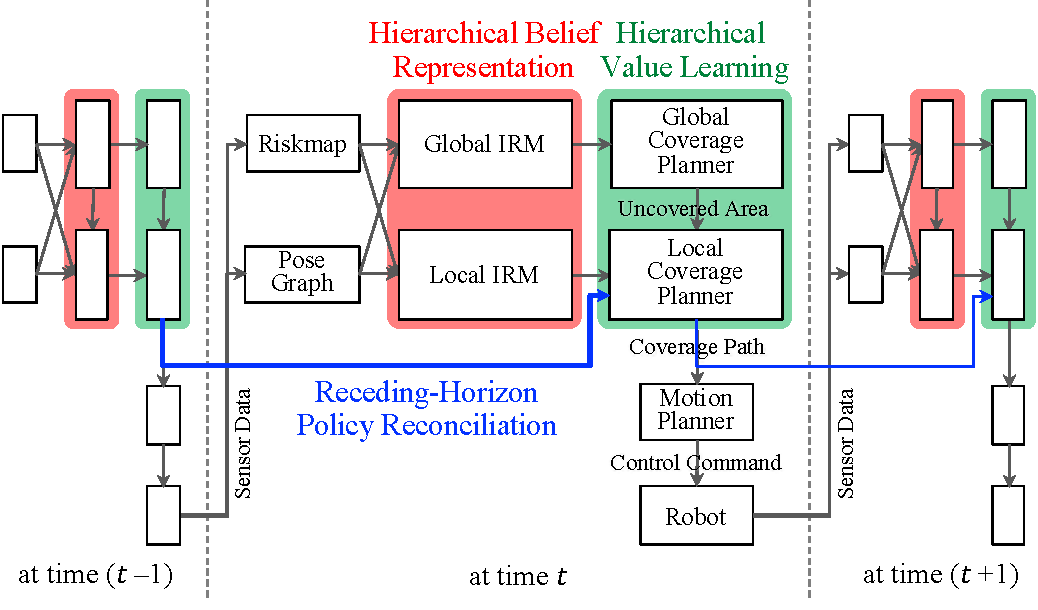
\includegraphics[width=\columnwidth]{figures/diagram.pdf}
  \caption{Illustration of PLGRIM framework for large-scale exploration in unknown environments.
  It \textit{i)} maintains hierarchical beliefs about the traversal risks and coverage states,
  \textit{ii)} performs hierarchical value learning to construct an exploration policy, and 
  \textit{iii)} reconciles policies over receding-horizon planning episodes.} 
  \label{fig:framework} 
\end{figure}




% \phdone{Formulation}
\subsection{Overview}
To enable efficient and reactive robot behaviors on very large scales, we decompose the problem into tractable subproblems by introducing spatial and temporal abstractions. Spatially, the belief space is approximated by a task-dependent structure, enriched with environment map estimates. Temporally, the belief space is approximated by the aggregation of multiple structures, each spanning a different spatial range. Finally, we introduce a cascaded optimization problem that returns a policy over the stratified belief space in real time. 

% stratification
% Spatially, the belief space is decomposed into task-relevant structures enriched with environment map estimates. Temporally, the belief space is decomposed into long-range and short-range structures.

% which enable efficient and reactive robot behaviors on very large scales

% (global) IRM which spans the entirety of the known environment,
% and a robot-centered short-range (local) IRM. We then propose a Receding Horizon Planning (RHP)-based solver to
% address the planning over this hierarchical POMDP structure in real time.
% We decompose the problem into tractable subproblems by introducing spatial and temporal abstractions which enable efficient and reactive robot behaviors on very large scales.
% We cast the coverage planning problem as a hierarchical POMDP problem in order to construct long-horizon, non-myopic action sequences. 
% The hierarchical architecture requires decomposition of the belief and policy spaces. 
% First, we decompose the belief state into local and global belief states. Then, given this belief decomposition, we define local and global policies that prescribes optimal action for each belief state.

% First, we formulate the hierarchical coverage planning in a POMDP setting.
%
% Let us decompose a belief state $b$ into local and global belief states, $b^\ell = (q, W^\ell)$ and $b^g = (q, W^g)$, respectively,
% Let us decompose a belief state $b$ into local and global belief states, $b^\ell = p((q, W^\ell))$ and $b^g = p((q, W^g))$, respectively.
% \ph{Belief Decomposition}
% \vspace{-2.5pt}
\subsubsection{Belief Decomposition:} \hfill
\vspace{-0.25pt}

\noindent
Let us denote the global world state as $W^g$ and the local world state as $W^\ell$, which is a subset of the global state, i.e., $W^\ell \subset W^g$, around the robot.
% We decompose the belief state $b$ into local and global belief states: $b^\ell = p(q, W^\ell)$ and $b^g = p(q, W^g)$, respectively.
We define local and global belief states as $b^\ell = p(q, W^\ell)$ and $b^g = p(q, W^g)$, respectively, where $p(W^\ell)$ is a local, robot-centric, rolling-window world belief representation with high-fidelity information, and $p(W^g)$ is a global, unbounded world belief representation with approximate information.

% \ph{Policy Decomposition}
% \subsubsection{4.1.2 Policy Decomposition} \hfill
% \vspace{-2.5pt}
\subsubsection{Policy Decomposition:} \hfill
\vspace{-0.25pt}

\noindent
We decompose the policy into local and global policies: $\pi^\ell$ and $\pi^g$, respectively. The overall policy $\pi \in \Pi$ is constructed by combining the local and global policies:
\begin{align}
  &\pi(b) = \pi^\ell(b^\ell; \pi^g(b^g)).
\end{align}
%
We approximate the original RHP optimization problem in Eq.~(\ref{eq:receding_objective_function}) as cascaded hierarchical optimization problems as follows:
\begin{align}
  &\pi_{t:t+T}(b)
  = \argmax_{\pi \in \Pi_{t:t+T}} \, \mathbb{E} \sum_{t'=t}^{t+T} \gamma^{t'-t} r(b_{t'}, \pi(b_{t'}))
  % = \argmax_{\pi^\ell \in \Pi^\ell_{t:t+T}} \, \mathbb{E} \sum_{t'=t}^{t+T} \gamma^{t'-t} r(b_{t'}, \pi^\ell(b^\ell_{t'}; \theta^\ell))
  \nonumber \\
  & \approx \argmax_{\pi^\ell \in \Pi^\ell_{t:t+T}} \, \mathbb{E} \sum_{t'=t}^{t+T} \gamma^{t'-t} r^\ell(b^\ell_{t'}, \pi^\ell(b^\ell_{t'}; \pi_{t:t+T}^g(b^g_t))),
  \label{eq:llp_optimization}
  \\
  &\text{where }
%   \pi_{t:t+T}^g(b^g) = \argmax_{\pi^g \in \Pi^g_{t:t+T}} \, \mathbb{E} \sum_{t'=t}^{t+T} \gamma^{t'-t} r^g(b^g_{t'}, \pi^g(b^g_{t'}))
  \pi_{t:t+T}^g(b^g) = \argmax_{\pi^g \in \Pi^g_{t:t+T}} \, \mathbb{E} \sum_{t'=t}^{t+T} \gamma^{t'-t} r^g(b^g_{t'}, \pi^g(b^g_{t'})).
  \label{eq:glp_optimization}
%   \label{eq:optimal_policy_unified}
\end{align}
\normalsize
% $\tilde{r}(b^g, \pi^g(b^g))$ is an approximate belief reward function for the global belief space.
where $r^\ell(b^\ell, \pi^\ell(b^\ell))$ and $r^g(b^g, \pi^g(b^g))$ are approximate belief reward functions for the local and global belief spaces, respectively.
%
Note that the codomain of the global policy $\pi^g(b^g)$ is a parameter space $\Theta^\ell$ of the local policy $\pi^\ell(b^\ell; \theta^\ell)$, $\theta^\ell \!\! \in \! \Theta^\ell\!$.\,

\phdone{Section Structure}
According to this formulation, we maintain the hierarchical belief representations (Section~\ref{ssec:belief-managers}) and solve for hierarchical POMDP policies (Section~\ref{ssec:belief-planners}).
For local planning consistency and resiliency, we extend Eq.~(\ref{eq:llp_optimization}) to a joint optimization problem given the previous planning episode policy (Section~\ref{ssec:resilient_rhp}).
% See Algorithm~\ref{alg:PLGRIM} for algorithmic description of the overall framework.


% \ph{Solver Formulation}
% We introduce some useful notations to describe the POMDP solvers.
% % As can be seen in Eq.~(\ref{eq:objective_function}), the objective of 
% The objective function, Eq.~(\ref{eq:objective_function}), is generally referred to as a \textit{value function}: 
% \begin{align}
%   V(b; \pi) &= \mathbb{E} \Big[ \sum_t \gamma^t r(b_t, \pi(b_t))] \Big],
% \end{align}
% % Value function:
% % % $V(b; \pi_{t:t+T0}) = \mathbb{E} [\sum_{t'=t}^{t+T} \gamma^{t'} r(b_{t'}, \pi_{t:t+T}(b_{t'}))]$
% % $V(b; \pi) = \mathbb{E} [\sum_t \gamma^t r(b_t, \pi(b_t))]$
% %
% or the expected reward when starting in belief $b$ and following policy $\pi$.
% From a recursive form of the \textit{value function}, we can define the value of taking action $a$ in belief $b$ under a policy $\pi$ by the \textit{action-value function}:
% \begin{align}
%   Q(b, a; \pi) = r(b, a) + \sum_{b' \in \mathbb{B}} \gamma \mathcal{T}(b, a, b') V(b'; \pi),
%   \label{eq:q_function}
% \end{align}
% where $\mathcal{T}(b, a, b')$ is the transition probability from $b$ to $b'$ by action $a$, as follows:
% % $\mathcal{T}(b, a, b') = \sum_{z \in \mathbb{Z}} p(b' | b, a, z) p(z | b, a)$ 
% \begin{align}
%   \mathcal{T}(b, a, b') = \sum_{z \in \mathbb{Z}} p(b' | b, a, z) p(z | b, a).
% \end{align}
% A POMDP solver tries to learn $Q(b, a)$ and $V(b) = \max_{a \in \mathbb{A}} Q(b, a)$, and returns the policy $\pi$ that specifies the best action for a given belief $b$, i.e., $\pi(b) = \argmax_{a \in \mathbb{A}} Q(b, a)$.

% Section 4.2: how to form local and global belief space 
% Section 4.3: how to solve optimization at each level
% Section 4.4: how to enhance the resiliency in the lower level



% \subsection{Hierarchical Belief Managers} \label{ssec:belief-managers}
\subsection{Hierarchical Belief Representation} \label{ssec:belief-managers}

\begin{algorithm}[t!]
% {\fontsize{9.2pt}{10.6pt}\selectfont
{\fontsize{8.5pt}{9.8pt}\selectfont
\caption{Hierarchical IRM Construction}
% \caption{PLGRIM: Information Roadmap Construction}
\label{alg:IRMs}
\begin{algorithmic}
  \STATE \textbf{input:} Riskmap, Pose Graph %, (estimated) robot pose %, Odometry

  \vspace{3pt}
  % \STATE \textbf{\# Local IRM}
  \STATE \textbf{\textit{\# Local IRM}}
  \STATE Local IRM $G^\ell = (N^\ell, E^\ell) \gets (\emptyset, \emptyset)$
  \STATE Add uniformly sampled nodes $\{n^\ell_i\}_i$ around the robot to $N^\ell$
  \FOR {each $n^\ell_i \in N^\ell$}
    % \STATE Compute risk probability $p(n^\ell_{i,r})$ from Riskmap
    % \STATE Compute coverage probability $p(n^\ell_{i,c})$ from Riskmap and Pose Graph by ray tracing
    \STATE Compute risk probability $p(n^\ell_{i,r})$ and coverage probability $p(n^\ell_{i,c})$ from Riskmap and Pose Graph for $n^\ell_i$
    \STATE Add $p(n^\ell_{i,r})$ and $p(n^\ell_{i,c})$ to the properties of $n^\ell_i$
  \ENDFOR
  \STATE Add edges for 8-connected neighbors, $\{e_{ij}\}^\ell_{i,j}$, to $E^\ell$
  \FOR {each $e^\ell_{ij} \in E^\ell$}
    \STATE Compute traversal risk $\rho_{ij}$ and distance $d_{ij}$ for $e^\ell_{ij}$
    \STATE Add $\rho_{ij}$ and $d_{ij}$ to the properties of $e^\ell_{ij}$
  \ENDFOR

  \vspace{3pt}
  % \STATE \textbf{\# Global IRM}
  \STATE \textbf{\textit{\# Global IRM}}
  \IF {not initialized}
    \STATE Global IRM $G^g = (N^g_b \cup N^g_f, E^g) \gets (\emptyset, \emptyset)$
    % \STATE initialized $\gets$ True
  \ENDIF
  
  \STATE Get the current robot pose $q$ from Pose Graph
  \IF {$q$ is farther from any breadcrumb node $\forall n^g_i \in N^g_b$ than $\bar{d}_b$}
%   \IF {$d(q, n^g) > \bar{d}_b$ for $\forall n^g \in N^g_b$}  % TODO: $d(\cdot, \cdot)$: distance function
    \STATE Add a new breadcrumb node $n^g = q$ to $N^g_b$
  \ENDIF


%   \STATE Get frontier nodes to add, $\hat{N}^g_{f^+}$, and frontier nodes to prune, $\hat{N}^g_{f^-}$, from FrontierManager given Riskmap and Pose Graph
  \STATE Run \textsc{FrontierManager} to add new frontiers $\{n^g_{f^+}\}$ with coverage probabilities $\{p(n^g_{f^+,c})\}$, and prune invalidated frontiers, $\{n^g_{f^-}\}$, based on the current Riskmap and Pose Graph
  \STATE \hspace{4.5cm} $\triangleright$ \cite{keidar2012robot}

  \FOR {each node $n^g_i \in \mathcal{N}_{G^g}(q)$}
%   \STATE $\triangleright \mathcal{N}_{G^g}(q)$: Nearby nodes of q in $G^g$
    % \STATE Compute the traversal distance $d_{ij}$ and risk $\rho_{ij}$ to its nearby nodes $\forall n^g_j \in \mathcal{N}_{G^g}(q)$
    \FOR {each nearby node $n^g_j \in \mathcal{N}_{G^g}(n^g_i)$}
      \STATE Compute the traversal distance $d_{ij}$ and risk $\rho_{ij}$
      \IF {$d_{ij} < \bar{d_e}$ and $\rho_{ij} < \bar{\rho_e}$}
        \STATE Add an edge $e^g_{ij}$ to $E^g$ with properties $d_{ij}$ and $\rho_{ij}$
      \ELSE
        \STATE Remove the edge $e^g_{ij}$ from $E^g$
      \ENDIF
    \ENDFOR
  \ENDFOR



  \vspace{3pt}
  \RETURN $G^\ell$ and $G^g$

\end{algorithmic}
} %fontsize environment
\end{algorithm}

\noindent
% To enable efficient representation of a large, rugged-terrain environment,
We introduce a hierarchical approximation of the belief space by decomposing the environment representation into multiple information-rich structures, each referred to as an Information Roadmap (IRM). 
% We decompose the world belief state into multiple representations, eac
% The hierarchical planner has two cascaded layers with different environment representation scales.
% decompose the world belief state into multiple representations, each encoding a different information resolution.
% To handle a large environmnet, we abstract primitive actions into large edges to be able to work with smaller stuctures. We call this IRM...
% For compact and versatile representation of the world, we choose a generic graph structure, $G = (N, E)$ with nodes $N$ and edges $E$, as the data structure to represent the belief about the world state.
% [NOTE: Avoid using $V$ to denote the set of nodes as $V$ is reserved for the value function.]
% We refer to this partitioning structure as the Information Roadmap (IRM).
% We refer to this representation as an Information RoadMap (IRM).
We construct and maintain IRMs at two hierarchical levels: the \textit{Local IRM} and \textit{Global IRM}, as illustrated in Fig.~\ref{fig:IRMs}. 
% Next, we provide a formal description how these IRMs encode the information about $W_{r}$ and $W_{c}$ at each level.

% \subsubsection{World Belief Formulation:} \hfill
% \vspace{-0.25pt}

% \noindent
% We denote the ground-truth world state by $W^*$.
% For unknown environment exploration, at any given time, the robot's understanding of the world is limited to $\hat{W} = p(W^g)$, a noise-susceptible estimate of the observed portions of the world.
% Note that $\hat{W}$ has two distinct attributes $\hat{W}_{r}$ and $\hat{W}_{c}$ that represent the risk and coverage states, respectively. The world state $\hat{W}$ can be partitioned into discrete spatial regions $\hat{W} = \{\hat{w}_i\}_i$, where each region $\hat{w}_i$ stores a risk and coverage value. 
% Assuming independence between $\hat{w}_i$, we approximate the world \textit{risk belief} and \textit{coverage belief} as the product of the marginal probabilities:
% \begin{align}
%   \!p(\hat{W}_{r}) = \Pi_i \, p(\hat{w}_{i,r}),\; \;~~
%   p(\hat{W}_{c}) = \Pi_i \, p(\hat{w}_{i,c}). 
%   \label{eq:coverage_belief}
% \end{align}

% \vspace{-2.5pt}
\subsubsection{World Belief Information Sources:} \hfill
\vspace{-0.25pt}

\noindent
% \ph{Information Sources}
% We denote the ground-truth world state by $W^*$.
During its exploration of an unknown environment, at any given time, the robot's understanding of the world is limited to noisy estimates of an observed subset of the world. 
% only the observed parts of the world. 
IRMs are constructed from these estimates--namely, the \textit{Riskmap} and \textit{Pose Graph}.
% Information to construct IRMs is sourced from other subsystems, which rely on this estimate. 
A Riskmap, constructed through the aggregation of point cloud sensor measurements, is a local rolling-window map that provides risk assessment, 
effectively encoding the risk belief over the local world state $W^\ell$ \cite{fan2021step}.
A Pose Graph
estimates the past trajectory of the robot from relative pose measurements and informs the coverage belief over the global world state $W^g$ \cite{Ebadi2020}. 

\subsubsection{World Belief Construction:} \hfill
\vspace{-0.25pt}

\noindent
For compact and versatile representation of the world, we choose a generic graph structure, $G = (N, E)$ with nodes $N$ and edges $E$, as the data structure to represent the belief about the world state. Using this framework, nodes represent discrete areas in space, and edges represent actions. More precisely, we define an action as a motion control from the current node $n_i \in N$ to a neighboring node $n_j \in N$, connected by an edge $e_{ij} \in E$.
% For example, if $a \in \mathbb{A}$ is a motion from node $\hat{w}_i \in N$ to node $\hat{w}_j \in N$ along edge $e_{ij} \in E$.

% % \ph{Information Sources}
% Information to construct IRMs is sourced from other subsystems. A \textit{Riskmap}, constructed through the aggregation of point cloud sensor measurements, is a local rolling-window map that provides risk assessment, %for a robot to be placed at each point of the map, 
% effectively encoding the risk belief $p(\hat{W}_{r}) = p(W^\ell_{r})$ over a local region \cite{fan2021step}.
% % It provides not only the estimated risk but also the confidence of the estimation for each point.
% % A \textit{Pose Graph} is a simple graph structure from SLAM (Simultaneous Localization and Mapping) module that provides the robot's past trajectory in global frame, 
% A \textit{Pose Graph} %, provided by the SLAM (Simultaneous Localization and Mapping) module, 
% estimates the past trajectory of the robot from relative pose measurements
% % represents the robot's past trajectory in the global coordinate frame, 
% and informs the coverage belief over the observed world, $p(\hat{W}_{c}) = p(W^g_{c})$ \cite{Ebadi2020}. 

For a detailed description of the Local and Global IRM construction processes, see Algorithm~\ref{alg:IRMs}. We now describe the distinguishing features of each IRM: 

\begin{enumerate}[label={\arabic*)}]
  \itemsep0em 
  \setlength{\itemsep}{0.2em}
%   \setlength{\parskip}{0pt}
  \item \textit{Local IRM}: 
As an instantiation of the local world belief $p(W^\ell)$, we employ a rolling, fixed-sized grid structure $G^\ell=(N^\ell, E^\ell)$, which is centered at the robot's current position.
We uniformly sample nodes $n^\ell_i \in N^\ell$ from $W^\ell$,
and compute the risk and coverage probability distribution over a discrete patch centered at each node, i.e.,
$p(n^\ell_{i,r})$ and $p(n^\ell_{i,c})$, which are stored as node properties. 
For an edge $e^\ell_{ij}$, we compute and store the traversal distance $d_{ij}$ and risk $\rho_{ij}$,
which effectively encodes $p(W^\ell_{r})$ between two connected nodes.
In summary, the Local IRM contains relatively high-fidelity information at a high resolution, but locally.

  \item \textit{Global IRM}:
As an instantiation of the global world belief $p(W^g)$, we employ a sparse bidirectional graph structure $G^g=(N^g, E^g)$, which is fixed in the global reference frame.
%   
%   Local IRM: batch
%   - Node sampling/generation (batch mode)
%   - Node properties
%   - Edge generation
%   - Edge properties
%  
%   Global IRM: online
%   - Node sampling condition check
%   - Edge connection condition check
%   - Node/edge generation
%   - Node/edge generation 
% 
%   Node sampling characteristics
%   : non-uniform, sparse sampling
%   : importantly, only when certain conditions are met
%     . breadcrumb: min distance from existing breadcrumbs
%     . frontier: on the border of covered and uncovered area
%     . both: existence of a traversable (low-risk) path
%   
%   Process
%   - Node sampling condition check
%   - Edge connection condition check
%   - Node/edge generation
%   - Node/edge generation 
Due to the space complexity concerns detailed in Section~\ref{ssec:challenges}, a densely-sampled grid structure, like $G^\ell$, is not a viable option for $G^g$, as it should span up to several kilometers.
% Instead, we sparsely and non-uniformly sample nodes $n^g_i \in N^g$ from $W^g$ based on certain node classifications. 
Instead, we sparsely and non-uniformly sample nodes $n^g_i \in N^g$ from $W^g$ based on certain node-classifying conditions. Specifically, $N^g$ contains two mutually exclusive subsets of nodes: \textit{breadcrumbs} 
% $N^g_b$ 
and \textit{frontiers}. 
% $N^g_f$. 
Breadcrumb nodes are sampled directly from the Pose Graph, and thus capture the \textit{covered traversable} space of $W^g$.
Alternatively, frontier nodes are sampled from the border between covered and uncovered areas, and thus capture the \textit{uncovered traversable} space of $W^g$. 
Finally, in order for such a candidate node $n^g_i$ to be added to $G^g$, there must exist a traversable path to at least one nearby node $n^g_j \in N^g$. If such a path exists, an edge $e^g_{ij}$, storing traversal distance $d_{ij}$ and risk $\rho_{ij}$, is added to $G^g$. 
See Fig.~\ref{fig:graph-level-planner} for identification of breadcrumb and frontier nodes in $G^g$.
% and the node $n^g_i$ is assigned a coverage probability $p(n^g_{i,c})$ property, indicative of its classification.
% , i.e., $\exists \; n^g_j \in \mathcal{N}_{G^g}(\hat{w}_i)$ such that the traversal risk $\rho_{ij}$ from $\hat{w}_i$ to $n^g_j$ is less than some positive threshold constant $\psi_e$: $\rho_{ij} \! \in \! [0, 1] < \psi_e$, where $\mathcal{N}_{G^g}(\cdot)$ is a set of nearby nodes in $G^g$. 
% In summary, the Global IRM captures the free-space connectivity of $W^g$ with a notion of coverage, and, in order to achieve compact representation of the large-scale environment, does not explicitly encode highly-likely untraversable or uncertain subspaces of $W^g$. 
In summary, the Global IRM captures the free-space connectivity of $W^g$ with a notion of coverage, and does not explicitly encode highly-likely untraversable or uncertain areas in $W^g$ in order to achieve compact representation of the large-scale environment. 

% 
% \begin{align}
%   &N^g_b \subset \{\hat{w}_i \, | \, p(\hat{w}_{i,\neg r} \wedge \hat{w}_{i,c}) > \psi_b\}, \\ %\notag \\
%   &N^g_f \subset \{\hat{w}_i \, | \, p(\hat{w}_{i,\neg r} \wedge \hat{w}_{i,\neg c}) > \psi_f\}, %\notag
%   \label{eq:breadcumb_frontier_definition}
% \end{align}

% where \psi_b$ and $\psi_f$ are positive threshold constants. Furthermore, in order for a candidate node $\hat{w}_i$ to be classified as either a breadcrumb or frontier, there must exist a traversable path to at least one nearby node in the Global IRM; $\exists \; n^g_j \in \mathcal{N}_{G^g}(\hat{w}_i)$ such that the traversal risk $\rho_{ij}$ from $\hat{w}_i$ to $n^g_j$ is less than some positive threshold constant $\psi_e$: $\rho_{ij} \! \in \! [0, 1] < \psi_e$, where $\mathcal{N}_{G^g}(\cdot)$ is a set of nearby nodes in $G^g$. In summary, the Global IRM captures the world's free-space connectivity with a notion of coverage, and, in order to achieve compact representation of the large-scale environment, it does not explicitly encode highly-likely occupied, untraversable, or uncertain subspaces of $\hat{W}$. Refer to Fig.~\ref{fig:graph-level-planner} for a visualization of breadcrumbs and frontier nodes in the Global IRM. 

% fig:graph-level-planner

\end{enumerate}

% \ph{Local Belief}
% An algorithmic description about Local and Global IRM construction is presented in Algorithm~\ref{alg:IRMs}.
%
% A Local IRM $G^\ell$ is rather straightforward to construct given a Riskmap and a Pose Graph.
% Once we have uniformly down-sampled nodes at $\{\hat{w}^\ell_i\}_i \subset \hat{W}^\ell$,
% we compute $p(\hat{w}^\ell_{i,r})$ and $p(\hat{w}^\ell_{i,c})$ from the Riskmap and Pose Graph for each node and encode them as node properties.
% For each edge to a neighbor node we compute a traversal risk and distance that effectively encodes $\hat{W}^\ell_{r}$ information between the two nodes.
% Hence, a Local IRM contains relatively high-fidelity information with a high resolution, but locally.



% \ph{Global Belief}
% Construction of a Global IRM $G^g$ needs more care, so that it can scale up to large $\hat{W}$, which may span up to several kilometers in this work.
% Thus, instead of a densely sampled graph, we use a sparse graph structure for a Global IRM.
% % A Global IRM is of a sparse graph structure, so that it can scale up to large $\hat{W}$, which may span up to several kilometers in this work.
% %
% It has two subsets of nodes, $N^g_b$ and $N^g_f$, so-called \textit{breadcrumb} and \textit{frontier} nodes, respectively, where $N^g_b \cap N^g_f = \emptyset$ and $N^g_b \cup N^g_f = N^g \! \subset \! \hat{W}$.
% %
% The breadcrumb nodes capture the \textit{covered free} space of $\hat{W}$, i.e., $N^g_b \subset \{\hat{w}_i | p(\hat{w}_{i,\neg r} \wedge \hat{w}_{i,c}) > \bar{\psi}_b\}$, while
% the frontier nodes capture the \textit{uncovered free} space, i.e., $N^g_f \subset \{\hat{w}_i | p(\hat{w}_{i,\neg r} \wedge \hat{w}_{i,\neg c}) > \bar{\psi}_f\}$,
% where $\bar{\psi}_b$ and $\bar{\psi}_f$ are some thresholds.
% %
% An additional condition for a candidate node $\hat{w}_i$ to be actually a breadcrumb or frontier node is that there should be a traversable path to nearby existing nodes in $G^g$, i.e., $\exists \hat{w}^g_j \in \mathcal{N}_{G^g}(\hat{w}_i)$ such that the traversal risk $\rho_{ij} \in [0, 1] < \bar{\psi}_e$ for $\hat{w}_i$ and $\hat{w}^g_j$, where $\mathcal{N}_{G^g}(\cdot)$ is a set of nearby nodes in $G^g$ and $\bar{\psi}_e$ is some threshold.
% %
% % In summary, we do not explicitly encode highly likely occupied, untraversable, or uncertain subspaces of $\hat{W}$ in a Global IRM for compact representation.
% In short, a Global IRM captures the free-space connectivity with a notion of coverage, and does not explicitly encode highly likely occupied, untraversable, or uncertain subspaces of $\hat{W}$ for compact representation of the large-scale world.
% %
% For a detailed description of Global IRM construction process, see Algorithm~\ref{alg:IRMs}.




\subsection{Hierarchical Value Learning} \label{ssec:belief-planners}

Given Local and Global IRMs as the hierarchical belief representation, we solve the cascaded hierarchical POMDP problems, Eq.~(\ref{eq:llp_optimization}) and Eq.~(\ref{eq:glp_optimization}), for coverage in an unknown environment.

% \ph{Solver Formulation}
% \vspace{-2.5pt}
\subsubsection{Solver Formulation:} \hfill
\vspace{-0.25pt}

\noindent
We start by introducing some notations.
% As can be seen in Eq.~(\ref{eq:objective_function}), the objective of 
% The objective function, Eq.~(\ref{eq:objective_function}), is generally referred to as a \textit{value function}: 
We define \textit{value function} $V(b; \pi)$ as the expected reward of following policy $\pi$, starting from belief $b$:
\begin{align}
  V(b; \pi) &= \mathbb{E} \Big[ \sum_t \gamma^t r(b_t, \pi(b_t))] \Big].
\end{align}
% Value function:
% % $V(b; \pi_{t:t+T0}) = \mathbb{E} [\sum_{t'=t}^{t+T} \gamma^{t'} r(b_{t'}, \pi_{t:t+T}(b_{t'}))]$
% $V(b; \pi) = \mathbb{E} [\sum_t \gamma^t r(b_t, \pi(b_t))]$
%
%
From a recursive form of the value function, we can define the value of taking action $a$ in belief $b$ under a policy $\pi$ by the \textit{action-value function}:
\begin{align}
  Q(b, a; \pi) = r(b, a) + \sum_{b' \in \mathbb{B}} \gamma \, \mathcal{T}(b, a, b') \, V(b'; \pi),
  \label{eq:q_function}
\end{align}
where $\mathcal{T}(b, a, b')$ is the transition probability from $b$ to $b'$ by action $a$, as follows:
% $\mathcal{T}(b, a, b') = \sum_{z \in \mathbb{Z}} p(b' | b, a, z) p(z | b, a)$ 
\begin{align}
  \mathcal{T}(b, a, b') = \sum_{z \in \mathbb{Z}} p(b' | b, a, z) \; p(z | b, a).
\end{align}
A POMDP solver tries to learn $Q(b, a)$ and $V(b) = \max_{a \in \mathbb{A}} Q(b, a)$, and returns the policy $\pi$ that specifies the best action for a given belief $b$, i.e., $\pi(b) = \argmax_{a \in \mathbb{A}} Q(b, a)$.



% \phdone{General POMDP Solver Formulation}
% We introduce some useful notations to describe the POMDP solvers.
% % As can be seen in Eq.~(\ref{eq:objective_function}), the objective of 
% The objective function, Eq.~(\ref{eq:objective_function}), is generally referred to as a \textit{value function}: 
% \begin{align}
%   V(b; \pi) &= \mathbb{E} \Big[ \sum_t \gamma^t r(b_t, \pi(b_t))] \Big],
% \end{align}
% % Value function:
% % % $V(b; \pi_{t:t+T0}) = \mathbb{E} [\sum_{t'=t}^{t+T} \gamma^{t'} r(b_{t'}, \pi_{t:t+T}(b_{t'}))]$
% % $V(b; \pi) = \mathbb{E} [\sum_t \gamma^t r(b_t, \pi(b_t))]$
% %
% or the expected reward when starting in belief $b$ and following policy $\pi$.
% From a recursive form of the \textit{value function}, we can define the value of taking action $a$ in belief $b$ under a policy $\pi$ by the \textit{action-value function}:
% \begin{align}
%   Q(b, a; \pi) = r(b, a) + \sum_{b' \in \mathbb{B}} \gamma \mathcal{T}(b, a, b') V(b'; \pi),
%   \label{eq:q_function}
% \end{align}
% where $\mathcal{T}(b, a, b')$ is the transition probability from $b$ to $b'$ by action $a$, as follows:
% % $\mathcal{T}(b, a, b') = \sum_{z \in \mathbb{Z}} p(b' | b, a, z) p(z | b, a)$ 
% \begin{align}
%   \mathcal{T}(b, a, b') = \sum_{z \in \mathbb{Z}} p(b' | b, a, z) p(z | b, a).
% \end{align}
% A POMDP solver tries to learn $Q(b, a)$ and $V(b) = \max_{a \in \mathbb{A}} Q(b, a)$, and returns the policy $\pi$ that specifies the best action for a given belief $b$, i.e., $\pi(b) = \argmax_{a \in \mathbb{A}} Q(b, a)$.

% \phdone{Reward Function--Information Gain}
% The reward function, Eq.~(\ref{eq:coverage_reward}), is concretely defined for our belief representation as follows.
% Given an IRM $G = (N, E)$ containing $p(\hat{w}_{i,c})$ value for each node $\hat{w}^\ell_i \in N^\ell$. 

% \ph{Solver Construction}
% \subsubsection{Solver Construction} \hfill
% \vspace{-2.5pt}
\subsubsection{Generalized Coverage Reward:} \hfill
\vspace{-0.25pt}

\noindent
% \ph{Coverage Information}
% The \textit{coverage belief} of the IRM $G = (N, E)$ containing nodes $\{\hat{w}_i, \cdots ,\hat{w}_k\} \in N$ is defined as: 
% \begin{align}
%     \nonumber
%     P_c(V) = \{p(\hat{w}_{i,c}), \cdots , p(\hat{w}_{k,c})\}
% \end{align}
% where $p_c(v_i)$ is the risk Bernoulli distribution over a local map centered at node $v_i$. 
% Given a \textit{coverage belief} in Eq.~(\ref{eq:coverage_belief}),  
Entropy provides a measure of uncertainty of a random variable's belief. Given an IRM $G = (N, E)$ containing a $p(n_{i,c})$ value for each node $n_i \in N$, the entropy of the world coverage state is:
% the amount of information needed to represent an event, given a belief. uncertainty of the coverage state can be represented as the entropy of the coverage belief. 
% Entropy of the world \textit{coverage belief} measures the uncertainty about the . The entropy of a random variable $x\sim p(x)$ is defined as $H_p(x) = E[-\log p(x)]$. Thus, the IRM coverage entropy is defined as:
\begin{multline}
  H(p(W_{c})) = - \sum_{i}^{|N|}\Big[ p(n_{i,c}) \log p(n_{i,c}) \\ 
  + p(n_{i,\neg c}) \log p(n_{i,\neg c}) \Big].
\end{multline}
% and the entropy in the belief of the world coverage state is defined as: 
% \begin{multline}
%   H(W^\ell_{c}) = - \sum_{i}^{|N^\ell|} \Big[ p(n^\ell_{i,c}) \log p(n^\ell_{i,c}) \\ 
%   + p(n^\ell_{i,\neg c}) \log p(n^\ell_{i,\neg c}) \Big]
% \end{multline}
% $H(W^\ell_{c}) = - \sum_{i}^{|N^\ell|} [ p(n^\ell_{i,c}) \log p(n^\ell_{i,c}) + p(n^\ell_{i,\neg c}) \log p(n^\ell_{i,\neg c}) ]$ 
% under the spatial independence assumption, so that we can compute the information gain $I(W^\ell_{c}, z)$ given an observation $z$.
% The same formulation applies to the Global IRM $G^g$ and $I(W^g_{c}, z)$.
If $a \in \mathbb{A}$ is a motion from node $n_i \in N$ to node $n_j \in N$ along edge $e_{ij} \in E$, then the coverage information gain (i.e., coverage uncertainty reduction) in \textit{coverage belief} $p(W_{c})$ induced by $a$ is defined as:
\begin{align}
    % I(\lambda(v_i), w_{c}) &= H_{p_{c}}(V) - H_{p_{c}}(V^\prime; \lambda(v_i), w_{c}) \\
    % I(\hat{W}_{c} \, | \, a) &= \underbrace{H(p(\hat{W}_{c}))}_\text{current entropy} - \underbrace{H(p(\hat{W}_{c})^\prime \, | \, a)}_\text{future entropy},
    I(W_{c} \, | \, a) &= \underbrace{H(p(W_{c}))}_\text{current entropy} - \underbrace{H(p(W_{c}\, | \, a))}_\text{future entropy},
\end{align}
where the second term represents the expected future entropy of the world coverage state after execution of action $a$. 

% Although the action cost function is instantiated at each hierarchical level according to the associated action set, it can be generically formulated as:
Although the action cost function at each hierarchical level is dependent upon the IRM's particular action set $E$ (i.e., Local and Global IRMs have different action sets), it can be generically formulated as:
% The action cost function is instantiated for the specific action set for each hierarchical level, but formulated in the same way. 
% For example, if $a \in \mathbb{A}$ is a motion from node $n_i \in N$ to node $n_j \in N$ along edge $e_{ij} \in E$.
% Let us omit the superscript $(\cdot)^\ell$ or $(\cdot)^g$ for notational brevity.
% In our framework, we define an action as a motion control from the current node to a neighbor node connected with an edge on the IRM.
% For example, if $a \in \mathbb{A}$ is a motion from node $n_i \in N$ to node $n_j \in N$ along edge $e_{ij} \in E$, then the action cost is computed as:
\begin{align}
    C(W_{r}, q, a) = k_d d_{ij} + k_\rho \rho_{ij} + k_\mu \mu_{ij}(q),
\end{align}
% $C(\hat{W}_{r}, q, a) = k_d d_{ij} + k_\rho \rho_{ij} + k_\mu \mu_{ij}(q)$,
where $d_{ij}$ and $\rho_{ij}$ are the traversal distance and risk along edge $e_{ij}$, respectively. The cost $\mu_{ij}(q)$ is associated with the current motion primitive, and is a consequence of the robot's non-holonomic constraints, such as the heading direction. Constants $k_d$, $k_\rho$, and $k_\mu$ weigh the importance of traversal distance, risk, and motion primitive history on the total action cost.

Then, finally the coverage reward function is defined as a weighted sum of the information gain and action cost:
\begin{align}
    R(s, a) = k_I I(W_{c}, z) - k_C \, C(W_{r}, q, a)),
\end{align}
where $k_I$ and $k_C$ are constant weights.



%% MANUALLY NUMBERED!
% \subsubsection{4.3.1. Global Coverage Planner} \label{sssec:GCP}
% \begin{figure}[t!]
%   \centering
%   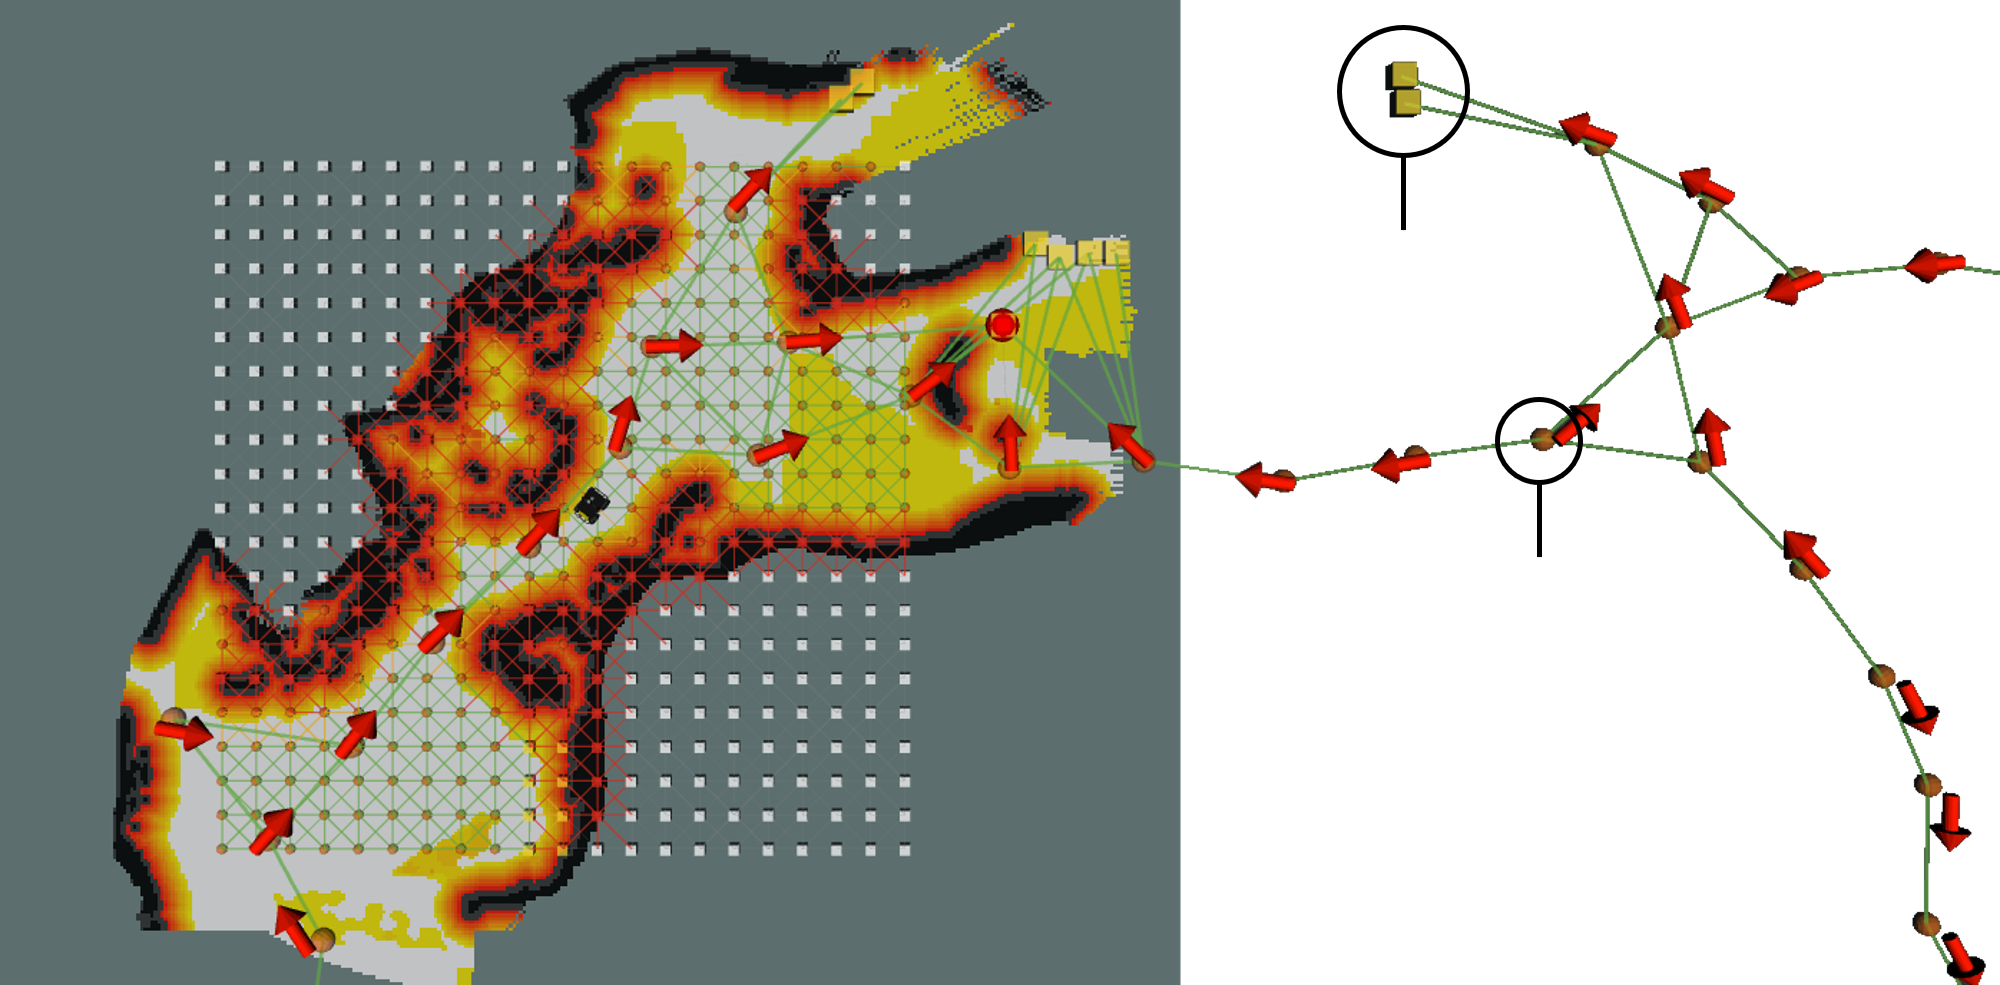
\includegraphics[width=1\columnwidth]{figures/QMDP_Policy_labels.png}
%   \caption{QMDP policy (red arrows displayed above \textit{breadcrumb} nodes) for Global Coverage Planning (GCP). A red sphere indicates the QMDP frontier goal.}
%   \label{fig:graph-level-planner}
% \end{figure}

\begin{figure}[t!]
\centering
    \begin{tikzpicture}
    \node[anchor=south west,inner sep=0] (image) at (0,0) {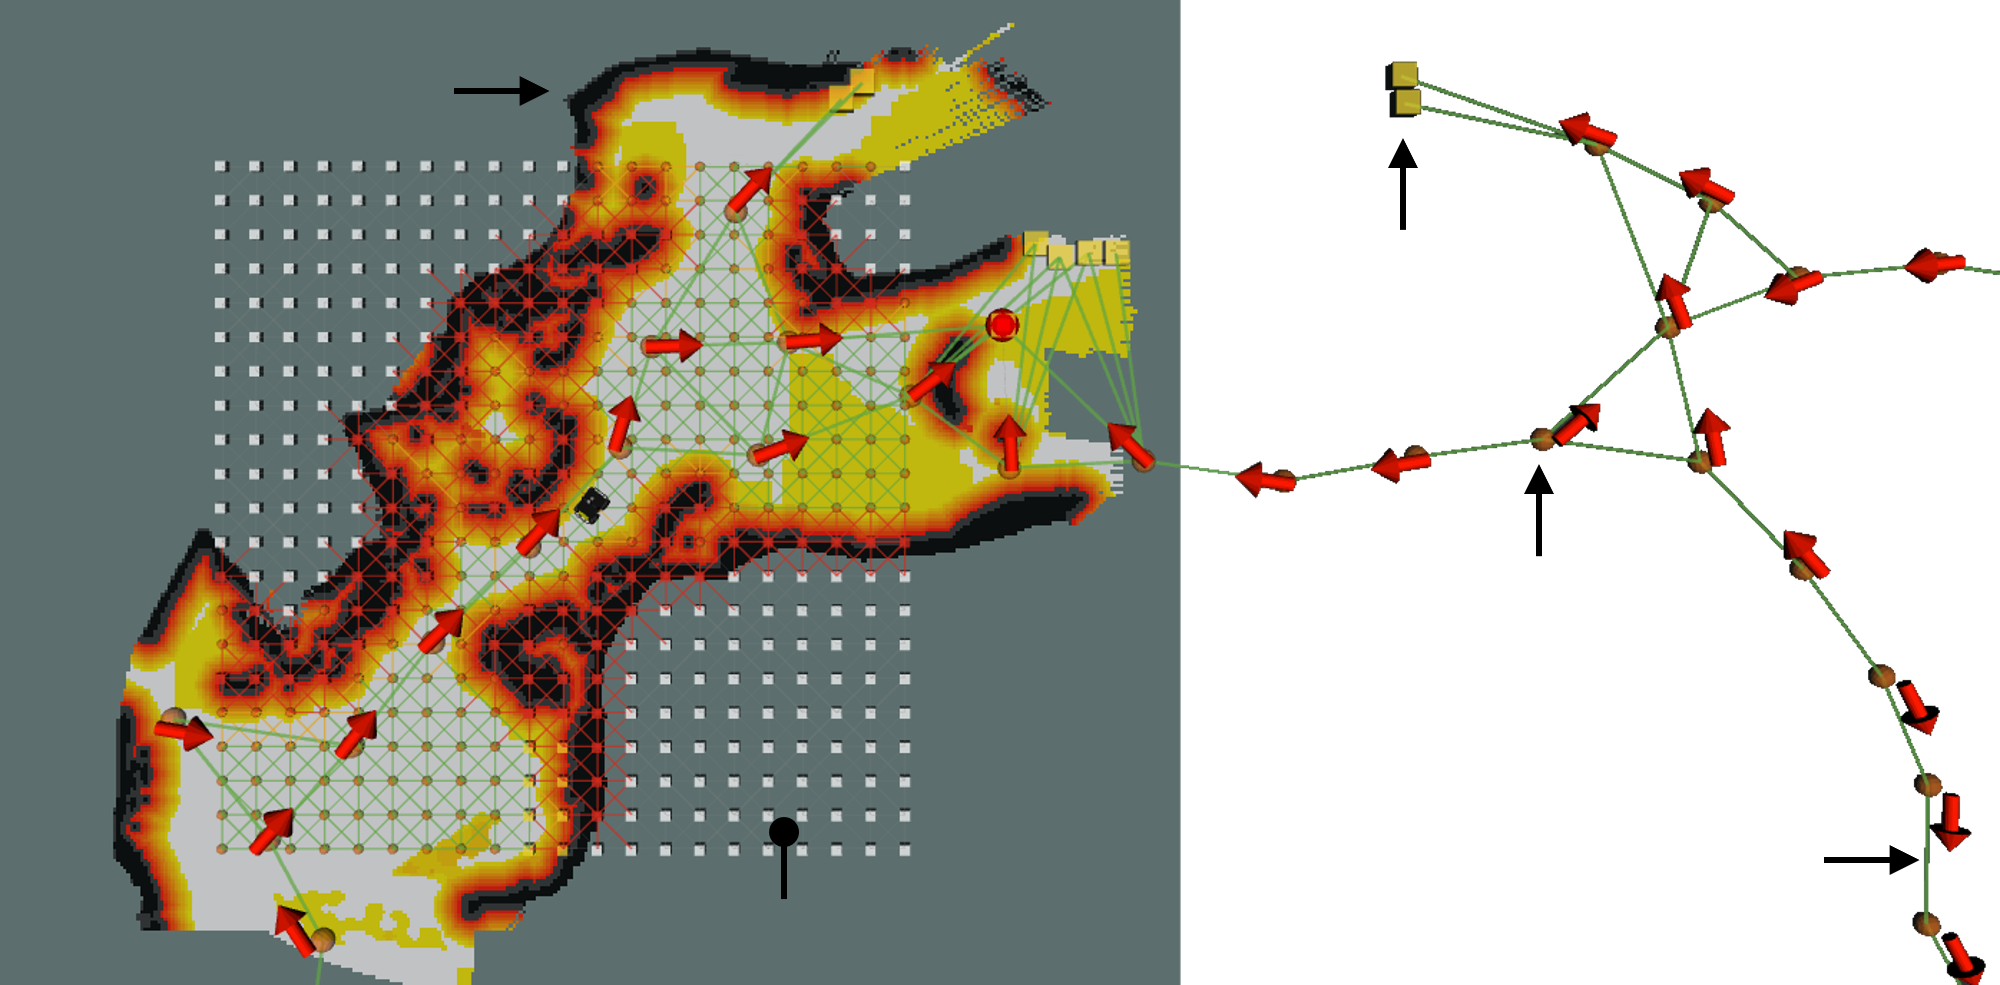
\includegraphics[width=1\columnwidth]{figures/QMDP_Policy_labels_v3.png}};
	    \begin{scope}[x={(image.south east)},y={(image.north west)}]
	    	
	    	% Annotations 
	    	\node [font=\scriptsize,above left,align=right,black] at (0.8,0.67) {Frontier Node}; 
	   % 	\node [font=\scriptsize,above left,align=right,black] at (0.76,0.615) {Cluster}; % we have no notion of clustering, so how about commenting out this line?
	    	\node [font=\scriptsize,above left,align=right,black] at (0.86,0.35) {Breadcrumb}; 
	    	\node [font=\scriptsize,above left,align=right,black] at (0.82,0.2915) {Node}; 
	    	\node [font=\scriptsize,above left,align=right,black] at (0.235,0.85) {Riskmap}; 
	    	\node [font=\scriptsize,above left,align=right,black] at (0.475,0.008) {Local IRM}; 
	    	\node [font=\scriptsize,above left,align=right,black] at (0.92,0.081) {Global IRM}; 

	    \end{scope}
	\end{tikzpicture}	
  \caption{QMDP policy (red arrows displayed above \textit{breadcrumb} nodes) for Global Coverage Planning (GCP). A red sphere indicates the QMDP frontier goal.}
  \label{fig:graph-level-planner}
\end{figure}


\begin{figure*}[h!]
\centering
    \begin{tikzpicture}
	    \node[anchor=south west,inner sep=0] (image) at (0,0) {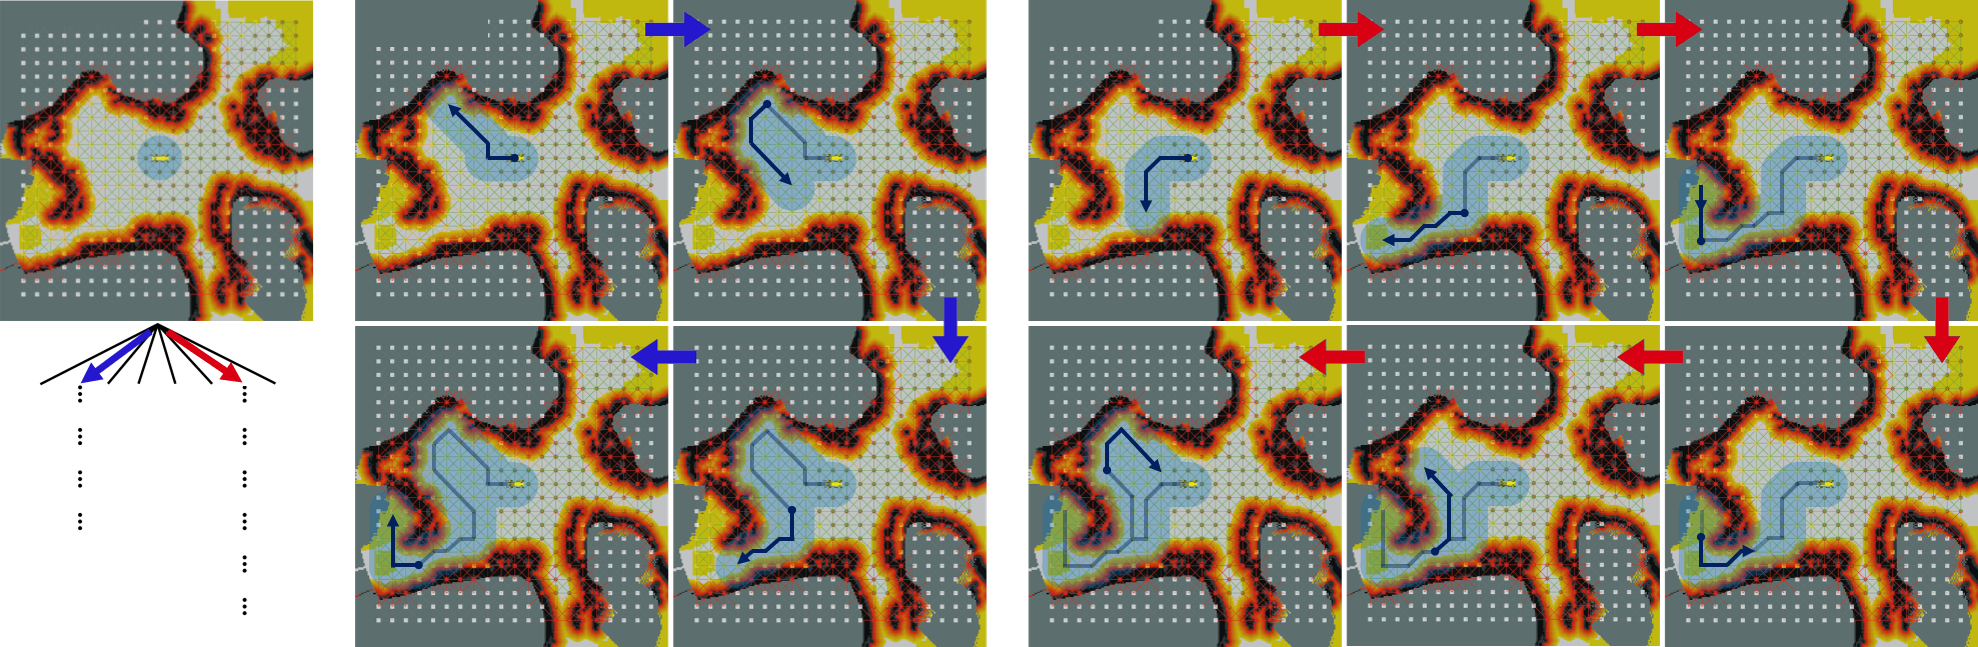
\includegraphics[width=1\textwidth]{figures/tree_figure_v9_ppt_v4}};
	    \begin{scope}[x={(image.south east)},y={(image.north west)}]
	    
    	    % Annotations [Big Labels]
	        \definecolor{mycolor_red}{RGB}{195.2, 0.0, 19.8}
	        \definecolor{mycolor_blue}{RGB}{37.2, 24, 204.6}
	        \node [above left,align=right,color=mycolor_blue] at (0.25,0.92) {Path $A$};
	        \node [above left,align=right,color=mycolor_red] at (0.59,0.92) {Path $B$};
	        \node [font=\scriptsize, above left,align=right,black] at (0.078,0.935) {Initial State};
	        
    	    % Annotations [W0]
	    	\node [font=\fontsize{4pt}{0}, above left,align=right,black] at (0.07,0.49) {$(W_0,Q_0)$};
	    	
    	    % Annotations [Tree]
	    	\node [font=\fontsize{4pt}{0}, above left,align=right,black] at (0.085,0.33) {$(W_{1a},Q_{1a})$};
	    	\node [font=\fontsize{4pt}{0}, above left,align=right,black] at (0.085,0.265) {$(W_{2a},Q_{2a})$};
	    	\node [font=\fontsize{4pt}{0}, above left,align=right,black] at (0.085,0.20) {$(W_{3a},Q_{3a})$};
	   % 	\node [font=\fontsize{4pt}{0}, above left,align=right,black] at (0.085,0.13) {$(W_{4a},Q_{4a})$};
	    	\node [font=\fontsize{4pt}{0}, above left,align=right,black] at (0.0835,0.13) {$(W_{1},Q_{4a})$};
	    	
	    	\node [font=\fontsize{4pt}{0}, above left,align=right,black] at (0.166,0.33) {$(W_{1b},Q_{1b})$};
	    	\node [font=\fontsize{4pt}{0}, above left,align=right,black] at (0.166,0.265) {$(W_{2b},Q_{2b})$};
	    	\node [font=\fontsize{4pt}{0}, above left,align=right,black] at (0.166,0.20) {$(W_{3b},Q_{3b})$};
	    	\node [font=\fontsize{4pt}{0}, above left,align=right,black] at (0.166,0.13) {$(W_{4b},Q_{4b})$};
	    	\node [font=\fontsize{4pt}{0}, above left,align=right,black] at (0.166,0.067) {$(W_{5b},Q_{5b})$};
	   % 	\node [font=\fontsize{4pt}{0}, above left,align=right,black] at (0.166,0.00) {$(W_{6b},Q_{6b})$};
	    	\node [font=\fontsize{4pt}{0}, above left,align=right,black] at (0.166,0.00) {$(W_{1},Q_{6b})$};
	    	
	    	% Annotations [Top]
	    	\node [font=\fontsize{4pt}{0}, above left,align=right,black] at (0.26,0.49) {$(W_{1a},Q_{1a})$};
	    	\node [font=\fontsize{4pt}{0}, above left,align=right,black] at (0.423,0.49) {$(W_{2a},Q_{2a})$};
	    	\node [font=\fontsize{4pt}{0}, above left,align=right,black] at (0.6,0.49) {$(W_{1b},Q_{1b})$};
	    	\node [font=\fontsize{4pt}{0}, above left,align=right,black] at (0.76,0.49) {$(W_{2b},Q_{2b})$};
	    	\node [font=\fontsize{4pt}{0}, above left,align=right,black] at (0.92,0.49) {$(W_{3b},Q_{3b})$};
	    	
	    	% Annotations [Bottom]
	   % 	\node [font=\fontsize{4pt}{0}, above left,align=right,black] at (0.26,-0.01) {$(W_{4a},Q_{4a})$};
	    	\node [font=\fontsize{4pt}{0}, above left,align=right,black] at (0.25,-0.01) {$(W_{1},Q_{4a})$};
	    	\node [font=\fontsize{4pt}{0}, above left,align=right,black] at (0.423,-0.01) {$(W_{3a},Q_{3a})$};
	    	\node [font=\fontsize{4pt}{0}, above left,align=right,black] at (0.59,-0.01) {$(W_{1},Q_{6b})$};
	    	\node [font=\fontsize{4pt}{0}, above left,align=right,black] at (0.76,-0.01) {$(W_{5b},Q_{5b})$};
	    	\node [font=\fontsize{4pt}{0}, above left,align=right,black] at (0.92,-0.01) {$(W_{4b},Q_{4b})$};
	    \end{scope}
	\end{tikzpicture}	
  \caption{Illustrative example of coverage path planning on the Local IRM with Monte-Carlo Tree Search. Robot field-of-view is represented by a blue circle. The state contains the world coverage state, $W_{c}$, and the robot state, $Q$. Macro actions (6 steps on Local IRM in this example) associated with two tree branches, paths \textit{A} and \textit{B}, are shown. Note that the final world coverage state $W_{c}$ in both branches are identical. Path \textit{A} is evaluated to be more rewarding than \textit{B} since fewer actions were required to cover the same area.}
  \label{fig:lattice-level-planner}
\end{figure*}


% \begin{enumerate}[label={\arabic*)}]
%   \itemsep0em 
%   \setlength{\itemsep}{0.2em}
% %   \setlength{\parskip}{0pt}
%   \item \textit{Global Coverage Planner}: 
% \phdone{GCP Functionality}
% In our cascaded hierarchical optimization framework, we first solve for the global policy in Eq.~(\ref{eq:glp_optimization}).
% As mentioned in Section~\ref{ssec:hierarchical_policy}, the outcome of the global policy is a parameter for the local policy.
% This means that Global Coverage Planner (GCP) for Eq.~(\ref{eq:glp_optimization}) provides \textit{global guidance} to Local Coverage Planner (LCP) for Eq.~(\ref{eq:llp_optimization}).
% The global guidance is for the coverage performance and completeness in a global sense, and especially helpful when there is no local area for LCP to cover.

% \phdone{GCP Problem Characteristics--Large-scale}
% There are special characteristics to note in global coverage planning. 
% First, the environment size can be very large (> 1~km), so GCP should be able to reason over more than hundreds of nodes on the Global IRM.
% %
% %
% \phdone{GCP Problem Characteristics--Frontiers as terminal nodes}
% Second, as the role of GCP is to guide the robot to an uncovered area and let LCP lead the local coverage behavior, GCP's policy search can terminate at frontier nodes on the Global IRM.
% %
% %
% \phdone{GCP Problem Approximation}
% Note that the second characteristic can help to mitigate the challenge from the first characteristic.
% By considering the frontier nodes as terminal nodes in the belief space, we can assume no changes to be made to the world coverage state before the termination, and thus, we can omit $W$ from the state space for GCP.
% Then, we can utilize simple and efficient POMDP solvers for a long horizon planning.


% \phdone{POMDP Solver for GCP}
% In this work, we adopt the QMDP approach for the global coverage planning \cite{littman1995learning}.
% The key idea of QMDP is to assume the state becomes fully observable after one step of action, so that the value function for further actions can be evaluated efficiently in an MDP (Markov Decision Process) setting.
% In our global coverage planning domain, we can consider the first step of action is for the robot to snap to one of the nearby node in Global IRM, and then, the robot pose is assumed to be fully observable, while the world risk and coverage states remain constant.


% \phdone{QMDP Details}
% More formally, we solve for $Q^g_{\mathrm{MDP}}(s^g, a^g)$ by ignoring uncertainty in robot pose $q^g$ and the change of $\hat{W}^g_{c}$, where $s^g \in N^g$ and $a^g$ is a control to move to a neighbor node $s'^g \in N^g$.
% In this MDP setting, $Q^g_{\mathrm{MDP}}(s^g, a^g)$ can be learned by Value Iteration very efficiently even for a long discount horizon.
% %
% Then, we can evaluate the Q-function in Eq.~(\ref{eq:q_function}) in a POMDP setting for the current belief and the feasible one-step actions, i.e.,
% $Q(b^g, a^g) = \int_{s^g} b(s^g) Q^g_{\mathrm{MDP}}(s^g, a^g) \mathrm{d}s^g$.
% %
% Finally, a POMDP policy can be obtained as follows:
% $\pi^g(b^g) = \argmax_{a^g \in \mathbb{A}^g} Q(b^g, a^g)$.
% %
% An example of the GCP policy is depicted in Fig.~\ref{fig:graph-level-planner}.
% % [TODO] See Algorithm~\ref{alg:PLGRIM} for more details.

%   \item \textit{Local Coverage Planner}:
% \phdone{LCP Functionality}
% In the hierarchical optimization framework, Local Coverage Planner (LCP) is who solves Eq.~(\ref{eq:llp_optimization}), given a parameter input from Global Coverage Planner (GCP).
% LCP constructs a high-fidelity policy by considering the information gathering (with visibility check given obstacles), traversal risk (based on proximity to obstacles, terrain roughness, and slopes), and robot's mobility constraints (such as acceleration limits and non-holonomic constraints of wheeled robots).


% \phdone{LCP Problem Characteristics}
% % LCP has multiple operation modes based on the parameter input $\theta^\ell \in \Theta^\ell = \mathbb{A}^g$ from GCP,
% LCP has multiple operation modes based on the parameter input $\theta^\ell = a^g \in \mathbb{A}^g$ from GCP,
% where the target frontier node in Global IRM, $n^g_f \in N^g$, can be extracted from the given global-level control $a^g$.
% %
% If $n^g_f$ is within the Local IRM range, i.e., $n^g_f \in \hat{W}^\ell$, then LCP performs the normal optimization as described in Eq.~(\ref{eq:llp_optimization}) for the local coverage behaviors.
% If $n^g_f \notin \hat{W}^\ell$, LCP simply instantiates a high-fidelity control of the given global-level control $a^g$ to follow the guidance of GCP.



% \phdone{POMDP Solver LCP}
% In order to solve Eq.~(\ref{eq:llp_optimization}) we employ POMCP (Partially Observable Monte Carlo Planning) algorithm \cite{silver2010monte}.
% POMCP is a widely-adopted POMDP solver that leverages the Monte Carlo sampling technique to alleviate both of the curse of dimensionality and history.
% Given a generative model (or a black box simulator) for discrete action and observation spaces, POMCP can learn the value function of near-optimally reachable belief space with adequate exploration-exploitation trade-off.


% \phdone{POMCP Details}
% More concretely, POMCP evaluates $Q^\ell(b^\ell, a^\ell)$ in Eq.~(\ref{eq:q_function}) by unrolling the recursive value backpropagation, with a set of sampled action-observation sequences.
% % [TODO] Provide a more concrete example with formulation.
% UCT algorithm for action selection helps to balance between exploration and exploitation to learn the Q-values.
% Initially it explored the search space (possible action-observation sequences) with a random or heuristically guided rollout policy.
% While incrementally building the belief tree it gradually exploits the learned values for more focused exploration with likely-optimal action-observation sequences (i.e., more focused exploration of the likely-reachable subspace by the optimal policy).
% See illustration of local coverage planning in Fig.~\ref{fig:lattice-level-planner}.
% \end{enumerate}

% \vspace{-2.5pt}
\subsubsection{Local-Global Coverage Planner Coordination:} \hfill
\vspace{-0.25pt}
% \subsubsection{Cascaded Local/Global Planner} \hfill

\noindent
In our cascaded hierarchical optimization framework, we first solve for the global policy in Eq.~(\ref{eq:glp_optimization}). The global policy solution then serves as an input parameter to the local policy in Eq.~(\ref{eq:llp_optimization}). This means that Global Coverage Planner (GCP) provides \textit{global guidance} to the Local Coverage Planner (LCP).

% In our cascaded hierarchical optimization framework, we first solve for the global policy in Eq.~(\ref{eq:glp_optimization}). The output of the global policy serves as a parameter for the local policy.

% This means that Global Coverage Planner (GCP), Eq.~(\ref{eq:glp_optimization}), provides \textit{global guidance} to Local Coverage Planner (LCP), Eq.~(\ref{eq:llp_optimization}).

% The global guidance is for the coverage performance and completeness in a global sense, and especially helpful when there is no local area for LCP to cover.

% \phdone{LCP Functionality}
% In the hierarchical optimization framework, Local Coverage Planner (LCP) is who solves Eq.~(\ref{eq:llp_optimization}), given a parameter input from Global Coverage Planner (GCP).

The role of GCP is to construct a low-fidelity policy that provides global guidance to uncovered areas, at which point, LCP instructs a local coverage behavior. More concretely, a target frontier node in the Global IRM, $n^g_f \in N^g_f$, can be extracted from the global-level control $a^g \in \mathbb{A}^g$ provided by GCP. Since the environment can be very large ($>\!\!1$~km), GCP must be capable of reasoning over hundreds of nodes on the Global IRM. To alleviate this scalability challenge, we assume that GCP's policy terminates at frontier nodes. By classifying frontier nodes as terminal in the belief space, we can assume no changes occur to the world coverage state before termination. Therefore, we omit $W$ from the state space for GCP.
% and can consequently utilize simple and efficient POMDP solvers for long horizon planning.
% 
% By considering the frontier nodes as terminal nodes in the belief space, we can assume no changes to be made to the world coverage state before the termination, and thus, we can omit $W$ from the state space for GCP.
% Then, we can utilize simple and efficient POMDP solvers for a long horizon planning.

% However, because LCP takes control, GCP's policy search can terminate at frontier nodes on the Global IRM.

% By considering the frontier nodes as terminal nodes in the belief space, we can assume no changes to be made to the world coverage state before the termination, and thus, we can omit $W$ from the state space for GCP.
% Then, we can utilize simple and efficient POMDP solvers for a long horizon planning.

% Since the environment can be very large (> 1~km), GCP must reason over hundreds of nodes on the Global IRM.

% \phdone{GCP Problem Characteristics--Large-scale}
% There are special characteristics to note in global coverage planning. 
% First, the environment size can be very large (> 1~km), so GCP should be able to reason over more than hundreds of nodes on the Global IRM.
%
%
% \phdone{GCP Problem Characteristics--Frontiers as terminal nodes}
% Second, as the role of GCP is to guide the robot to an uncovered area and let LCP lead the local coverage behavior, GCP's policy search can terminate at frontier nodes on the Global IRM.
% %
% %
% \phdone{GCP Problem Approximation}
% Note that the second characteristic can help to mitigate the challenge from the first characteristic.
% By considering the frontier nodes as terminal nodes in the belief space, we can assume no changes to be made to the world coverage state before the termination, and thus, we can omit $W$ from the state space for GCP.
% Then, we can utilize simple and efficient POMDP solvers for a long horizon planning.
% 
% The role of LCP is to construct a high-fidelity policy that provides local guidance \st{to uncovered areas} by considering information gathering (with visibility check given obstacles), traversal risk (based on proximity to obstacles, terrain roughness, and slopes), and the robot's mobility constraints (such as acceleration limits and non-holonomic constraints of wheeled robots).
The role of LCP is to construct a high-fidelity policy that provides local guidance based on information gathering, traversal risk (e.g., proximity to obstacles, terrain roughness, and slopes), and the robot's mobility constraints (e.g., acceleration limits and non-holonomic constraints of wheeled robots).
% \phdone{LCP Problem Characteristics}
% LCP has multiple operation modes based on the parameter input $\theta^\ell \in \Theta^\ell = \mathbb{A}^g$ from GCP,
% \sout{
% In practice, LCP has two operational modes based on GCP's guidance: one that prioritizes information-gathering and one that prioritizes global target realization.
% % 
% % Specifically, a target frontier node in the Global IRM, $n^g_f \in N^g$, can be extracted from the global-level control $a^g$.
% %
% If the target frontier $n^g_f$ is within the Local IRM range, i.e., $n^g_f \in \hat{W}^\ell$, then the first mode is activated, and LCP performs the normal information-gathering coverage optimization, as described in Eq.~(\ref{eq:llp_optimization}).
% However, if $n^g_f \notin \hat{W}^\ell$, LCP simply instantiates high-fidelity control  based on the global-level control $a^g$ in order to achieve the target frontier.
% }
LCP has two phases: i) reach the target area based on GCP's guidance, and ii) construct a local coverage path after reaching the target area.
If the target frontier is outside the Local IRM range, i.e., $n^g_f \notin W^\ell$, LCP simply instantiates high-fidelity control  based on the global-level control $a^g$ in order to reach the target frontier.
If the target frontier $n^g_f$ is within the Local IRM range, i.e., $n^g_f \in W^\ell$, then LCP performs the nominal information-gathering coverage optimization, as described in Eq.~(\ref{eq:llp_optimization}).


% \subsubsection{4.3.1. Global Coverage Planner} \label{sssec:GCP}
% \vspace{-2.5pt}
\subsubsection{Global Coverage Planner (GCP) Algorithm:}\label{sssec:GCP} \hfill
\vspace{-0.25pt}
% \phdone{GCP Functionality}
% In our cascaded hierarchical optimization framework, we first solve for the global policy in Eq.~(\ref{eq:glp_optimization}).
% As mentioned in Section~\ref{ssec:hierarchical_policy}, the outcome of the global policy is a parameter for the local policy.
% This means that Global Coverage Planner (GCP) for Eq.~(\ref{eq:glp_optimization}) provides \textit{global guidance} to Local Coverage Planner (LCP) for Eq.~(\ref{eq:llp_optimization}).
% The global guidance is for the coverage performance and completeness in a global sense, and especially helpful when there is no local area for LCP to cover.

% \phdone{GCP Problem Characteristics--Large-scale}
% There are special characteristics to note in global coverage planning. 
% First, the environment size can be very large (> 1~km), so GCP should be able to reason over more than hundreds of nodes on the Global IRM.
% %
% %
% \phdone{GCP Problem Characteristics--Frontiers as terminal nodes}
% Second, as the role of GCP is to guide the robot to an uncovered area and let LCP lead the local coverage behavior, GCP's policy search can terminate at frontier nodes on the Global IRM.
% %
% %
% \phdone{GCP Problem Approximation}
% Note that the second characteristic can help to mitigate the challenge from the first characteristic.
% By considering the frontier nodes as terminal nodes in the belief space, we can assume no changes to be made to the world coverage state before the termination, and thus, we can omit $W$ from the state space for GCP.
% Then, we can utilize simple and efficient POMDP solvers for a long horizon planning.
\noindent
% \phdone{POMDP Solver for GCP}
In this work, we adopt the QMDP approach for the global coverage planning \cite{littman1995learning}.
The key idea of QMDP is to assume the state becomes fully observable after one step of action, so that the value function for further actions can be evaluated efficiently in an MDP (Markov Decision Process) setting.
In our global coverage planning domain, we define the first action to be the robot's relocation to a nearby node on the Global IRM, and then, the robot pose is assumed to be fully observable, while the world risk and coverage states remain unchanged.


\phdone{QMDP Details}
More formally, we solve for $Q^g_{\mathrm{MDP}}(s^g, a^g)$ by ignoring uncertainty in robot pose $q^g$ and the change of $W^g_{c}$, where $s^g \in N^g$ and $a^g$ is a control to move to a neighbor node $s'^g \in N^g$.
In this MDP setting, $Q^g_{\mathrm{MDP}}(s^g, a^g)$ can be learned by Value Iteration very efficiently even for a long discount horizon.
%
Then, we can evaluate the \textit{action-value function} in Eq.~(\ref{eq:q_function}) in a POMDP setting for the current belief and the feasible one-step actions:
\begin{align}
  Q(b^g, a^g) = \int_{s^g} b(s^g) Q^g_{\mathrm{MDP}}(s^g, a^g) \mathrm{d}s^g.
\end{align}
% $Q(b^g, a^g) = \int_{s^g} b(s^g) Q^g_{\mathrm{MDP}}(s^g, a^g) \mathrm{d}s^g$.
%
Finally, a POMDP policy can be obtained as follows:
\begin{align}
  \pi^g(b^g) = \argmax_{a^g \in \mathbb{A}^g} Q(b^g, a^g).
\end{align}
% $\pi^g(b^g) = \argmax_{a^g \in \mathbb{A}^g} Q(b^g, a^g)$.
%
An example of the GCP policy is depicted in Fig.~\ref{fig:graph-level-planner}.
% [TODO] See Algorithm~\ref{alg:PLGRIM} for more details.



% MANUALLY NUMBERED!
% \subsubsection{4.3.2. Local Coverage Planner} \label{sssec:LCP}
% \phdone{LCP Functionality}
% In the hierarchical optimization framework, Local Coverage Planner (LCP) is who solves Eq.~(\ref{eq:llp_optimization}), given a parameter input from Global Coverage Planner (GCP).
% LCP constructs a high-fidelity policy by considering the information gathering (with visibility check given obstacles), traversal risk (based on proximity to obstacles, terrain roughness, and slopes), and robot's mobility constraints (such as acceleration limits and non-holonomic constraints of wheeled robots).


% \phdone{LCP Problem Characteristics}
% % LCP has multiple operation modes based on the parameter input $\theta^\ell \in \Theta^\ell = \mathbb{A}^g$ from GCP,
% LCP has multiple operation modes based on the parameter input $\theta^\ell = a^g \in \mathbb{A}^g$ from GCP,
% where the target frontier node in Global IRM, $n^g_f \in N^g$, can be extracted from the given global-level control $a^g$.
% %
% If $n^g_f$ is within the Local IRM range, i.e., $n^g_f \in \hat{W}^\ell$, then LCP performs the normal optimization as described in Eq.~(\ref{eq:llp_optimization}) for the local coverage behaviors.
% If $n^g_f \notin \hat{W}^\ell$, LCP simply instantiates a high-fidelity control of the given global-level control $a^g$ to follow the guidance of GCP.

% \vspace{-2.5pt}
\subsubsection{Local Coverage Planner (LCP) Algorithm:}\label{sssec:LCP} \hfill
\vspace{-0.25pt}

\noindent
% \phdone{POMDP Solver LCP}
In order to solve Eq.~(\ref{eq:llp_optimization}), we employ POMCP (Partially Observable Monte Carlo Planning) algorithm \cite{silver2010monte}.
POMCP is a widely-adopted POMDP solver that leverages the Monte Carlo sampling technique to alleviate both of the \textit{curse of dimensionality} and \textit{history}.
Given a generative model (or a black box simulator) for discrete action and observation spaces, POMCP can learn the value function of near-optimally reachable belief space with adequate exploration-exploitation trade-off.


\phdone{POMCP Details}
More concretely, POMCP evaluates $Q^\ell(b^\ell, a^\ell)$ in Eq.~(\ref{eq:q_function}) by unrolling the recursive value backpropagation, with a set of sampled action-observation sequences.
% [TODO] Provide a more concrete example with formulation.
UCT algorithm for action selection helps to balance between exploration and exploitation to learn the \textit{action-value function}.
Initially, it explores the search space (possible action-observation sequences) with a random or a heuristically guided rollout policy.
While incrementally building the belief tree, it gradually exploits the learned values for more focused exploration with likely-optimal action-observation sequences (i.e., more focused exploration of the likely-reachable subspace by the optimal policy).
See illustration of local coverage planning in Fig.~\ref{fig:lattice-level-planner}.




% \subsection{Resilient Receding Horizon Planning} \label{ssec:resilient_rhp}
\subsection{Receding-Horizon Policy Reconciliation} \label{ssec:resilient_rhp}

\phdone{Consistency and Resiliency}
We extend the receding-horizon \textit{local} coverage planning problem to address the trade-off between policy consistency and resiliency, as described in Section~\ref{ssec:challenges}.
% \textit{Policy Concatenation}.
% \textit{Policy Reconciliation}.
% \textit{Unexpected Belief Updates}.

% over consecutive plans to avoid unnecessary rotations, slow-down, or back-and-forth motions,
% and \textit{resiliency} in a new plan in the presence of unforeseen hazard or anomalies.
% % Consistency is related to how conformable the beginning of the new policy is to the end of the previous policy, while resiliency is related to 
% In normal operations, consistency is preferred so that the robot can move effectively and make greater mission progress, while in abnormal situations, resiliency is required to ensure to the robot's safety and adapt to the unexpected changes.


\phdone{Receding Horizon Planning Re-formulation}
% We define a policy reconciliation optimization problem by introducing the previous planning episode policy generated at time ($t-\Delta t$) into Eq.~(\ref{eq:receding_objective_function}), for the current planning episode at time $t$.
We define a policy reconciliation optimization problem by introducing the previous planning episode policy into Eq.~(\ref{eq:receding_objective_function}) for the current planning episode.
% We define a policy reconciliation optimization problem by introducing the previous planning episode policy into current planning episode policy, as described by Eq.~(\ref{eq:receding_objective_function}).
% Eq.~(\ref{eq:llp_optimization}).
% Let us denote the current time $t_1$ and the previous planning time $(t_1-\Delta t)$ as $t_0$ for notational brevity.
For notational brevity, let us denote the time when the previous policy was generated as $t_0$ and the current time as $t_1 = t_0 + \Delta t$.
% For notational brevity, let us denote the current time as $t_1$ and $t_1-\Delta t$ as $t_0$.
%
% $\pi_{t:t+T}^*(b; \pi_{t_0:t_0+T}^-)$, where $\pi_{t_0:t_0+T}^-$ is the previous policy constructed at time $t_0$ for a finite horizon with a length of $T$.
%
% $\pi_{t:t+T}^*(b; \pi_{t-\Delta t:t-\Delta t+T}^-)$, where $\pi_{t-\Delta t:t-\Delta t+T}^-$ is the previous policy constructed at time $(t - \Delta t)$ for a finite horizon with a length of $T$.
% $\pi_{t:t+T}^*(b; \pi_{t-\Delta t:t-\Delta t+T}^-) = \argmax_{\pi \in \Pi_{t:t+T}} \, \mathbb{E} \sum_{t'=t}^{t+T} \gamma^{t'-t} r(b_{t'}, \pi(b_{t'}; \pi_{t-\Delta t:t-\Delta t+T}^-))$.
%
%
% Given the previous policy $\pi_{t_0:t_0+T}^-$ constructed at time $t_0$ with a finite horizon of $T$,
% we extend Eq.~(\ref{eq:receding_objective_function}) as below 
% in order to find a balance between policy consistency and resiliency over receding horizons.
In order to reconcile consecutive policies over receding horizons, we extend Eq.~(\ref{eq:receding_objective_function}) as follows, given the previous policy $\pi_{t_0:t_0+T}^-$ constructed at time $t_0$ for a finite horizon of $T$:
%
% \begin{align}
%   \pi_{t:t+T}^*(b) &= \argmax_{\pi \in \Pi_{t:t+T}} \, \mathbb{E} \sum_{t'=t}^{t+T} \gamma^{t'-t} r(b_{t'}, \pi(b_{t'})),
% \end{align}
% \begin{align}
%   &\pi_{t:t+T}^*(b; \pi_{t-\Delta t:t-\Delta t+T}^-) 
%   \nonumber \\
%   &= \argmax_{\pi \in \Pi_{t:t+T}} \, \mathbb{E} \sum_{t'=t}^{t+T} \gamma^{t'-t} r(b_{t'}, \pi(b_{t'}; \pi_{t-\Delta t:t-\Delta t+T}^-)),
%   \label{eq:revised_receding_objective_function}
% \end{align}
%
% \begin{align}
%   \pi_{t_1:t_1+T}^*(b) &= \argmax_{\pi \in \Pi_{t_1:t_1+T}} \, \mathbb{E} \sum_{t'=t_1}^{t_1+T} \gamma^{t'-t_1} r(b_{t'}, \pi(b_{t'})),
% \end{align}
% \begin{align}
%   &\pi_{t_1:t_1+T}^*(b; \pi_{t_0:t_0+T}^-) 
%   \nonumber \\
%   &= \argmax_{\pi \in \Pi_{t_1:t_1+T}} \, \left[ \mathbb{E} \sum_{t'=t_1}^{t_1+T} \gamma^{t'-t_1} r(b_{t'}, \pi(b_{t'})) \right.
%   \nonumber \\
%   & \qquad\qquad\qquad\,\,\,\, \left. - \lambda \mathcal{R}(\pi_{t_0:t_0+T}^-, \pi_{t_1:t_1+T}) \right],
%   \label{eq:revised_receding_objective_function}
% \end{align}
\begin{multline}
  \pi_{t_1:t_1+T}^*(b; \pi_{t_0:t_0+T}^-) 
  \\
  = \argmax_{\pi \in \Pi_{t_1:t_1+T}} \, \left[ \mathbb{E} \sum_{t'=t_1}^{t_1+T} \gamma^{t'-t_1} r(b_{t'}, \pi(b_{t'})) \right.
  \\
   \left. - \lambda \mathcal{R}(\pi_{t_0:t_0+T}^-, \pi_{t_1:t_1+T}) \right],
  \label{eq:revised_receding_objective_function}
\end{multline}
where $\mathcal{R}(\pi_{t_0:t_0+T}^-, \pi_{t_1:t_1+T})$ is a regularizing cost function that penalizes inconsistency between the previous and current policies in terms of kinodynamic constraints, and $\lambda$ is a regularization weight parameter.
The first term in Eq.~(\ref{eq:revised_receding_objective_function}) pursues policy resiliency based on the up-to-date world belief, which may encode unexpected hazards, while the second term promotes policy consistency.

% Based on our observation that the conflict between policy consistency and resiliency is most dominant
Since the conflict between policy consistency and resiliency is most severe
at the junction between two consecutive policies,
we decompose Eq.~(\ref{eq:revised_receding_objective_function}) into two time frames, $(t_1:t_1+\tau)$ and $(t_1+\tau:t_1+T)$ for $\tau \in [0,\, T-\Delta t]$, and formulate it as a simplified joint optimization problem for $\tau^*$ and $\pi_{t_1+\tau^*:t_1+T}^*$:
%
% We define an optimization variable $\tau_t$ that controls how much the new policy should observe the previous policy for the consistency 
% We define another optimization variable $\tau_t$ that specifies how long the new policy should comply with the previous policy.
% A larger $\tau_t$ will enforce path consistency, while a smaller $\tau_t$ will enhance path resiliency.
%
% Here we consider a joint optimization problem how much of the previous policy should be preserved as follows:
% \begin{align}
%   % &\left(\pi_{t:t+T}^*(b; \pi_{{t'}-\Delta t:{t'}-\Delta t+T}^*), \, \tau_t^*\right)
%   % &\left(\pi_{t:t+T}^*, \, \tau_t^*\right)
%   &(\pi_{t:t+T}^*, \, \tau_t^*)
%   \nonumber \\
%   & = \argmax_{\pi \in \Pi_{t:t+T}, \, \tau \in [0, T-\Delta t]} \, \mathbb{E} \sum_{t'=t}^{t+\tau} \gamma^{t'-t} r(b_{t'}, \pi(b_{t'}; \pi_{{t'}-\Delta t:{t'}+T-\Delta t}^-))
%   \nonumber \\
%   &\quad + \sum_{t'=t+\tau}^{t+T} \gamma^{t'-t} r(b_{t'}, \pi(b_{t'}))
%   % \\
%   % & = \argmax_{\pi \in \Pi_{t:t+T}, \, \tau \in [0, T-\Delta t]} \, \mathbb{E} \sum_{t'=t}^{t+\tau} \gamma^{t'-t} r(b_{t'}, \pi_{{t'}-\Delta t:{t'}+T-\Delta t}^-(b_{t'}))
%   % \nonumber \\
%   % &\quad + \sum_{t'=t+\tau}^{t+T} \gamma^{t'-t-\tau} r(b_{t'}, \pi(b_{t'})),
% \end{align}
%
%
%
% A joint optimization problem for $\pi_{t:t+T}^*$ and $\tau_t^*$ for a planning episode at time $t$ can be described as follows:
% \begin{align}
%   &(\pi_{t:t+T}^*, \, \tau_t^*) = \argmax_{\pi \in \Pi_{t:t+T}, \, \tau \in [0, T-\Delta t]}
%   \nonumber \\
%   &  \, \mathbb{E} \sum_{t'=t}^{t+\tau} \gamma^{t'-t} r(b_{t'}, \pi(b_{t'}; \pi_{{t'}-\Delta t:{t'}+T-\Delta t}^-))
%   \nonumber \\
%   &\quad + \sum_{t'=t+\tau}^{t+T} \gamma^{t'-t} r(b_{t'}, \pi(b_{t'}))
% \end{align}
%
% \begin{align}
%   &(\pi_{t:t+T}^*, \, \tau_t^*)
%   \nonumber \\
%   & = \argmax_{\pi \in \Pi_{t:t+T}, \, \tau \in [0, T-\Delta t]} \, \mathbb{E} \sum_{t'=t}^{t+\tau} \gamma^{t'-t} r(b_{t'}, \pi(b_{t'}; \pi_{{t'}-\Delta t:{t'}+T-\Delta t}^-))
%   \nonumber \\
%   &\quad + \sum_{t'=t+\tau}^{t+T} \gamma^{t'-t} r(b_{t'}, \pi(b_{t'}))
% \end{align}
%
% \begin{align}
%   &(\pi_{t:t+T}^*, \, \tau_t^*)%   \nonumber \\
%   & = \argmax_{\pi \in \Pi_{t:t+T}, \, \tau \in [0, T-\Delta t]} \, \mathbb{E} \Biggl[ \sum_{t'=t+\tau}^{t+T} \gamma^{t'-t} r(b_{t'}, \pi(b_{t'}))
%   \nonumber \\
%   &\quad + \sum_{t'=t}^{t+\tau} \gamma^{t'-t} r(b_{t'}, \pi(b_{t'}; \pi_{{t'}-\Delta t:{t'}+T-\Delta t}^-)) \Biggr]
% \end{align}
%
%
% LATEST VERSION
% \begin{align}
%   &(\pi_{t:t+T}^*, \, \tau_t^*)
%   \nonumber \\
%   & = \argmax_{\pi \in \Pi_{t:t+T}, \, \tau \in [0,\, T-\Delta t]} \, \mathbb{E} \left[ \sum_{t'=t+\tau}^{t+T} \gamma^{t'-t} r(b_{t'}, \pi(b_{t'})) \right.
%   \nonumber \\
%   &\quad \left. + \sum_{t'=t}^{t+\tau} \gamma^{t'-t} r(b_{t'}, \pi(b_{t'}; \pi_{{t'}-\Delta t:{t'}+T-\Delta t}^-)) \right] \!\!.
%   \label{eq:resiliency_optimization}
% \end{align}
%
% \begin{align}
%   & \maximize_{\pi \in \Pi_{t:t+T}, \, \tau \in [0,\, T-\Delta t]} \, \mathbb{E} \left[ 
%   \sum_{t'=t}^{t+\tau} \gamma^{t'-t} r(b_{t'}, \pi(b_{t'}; \pi_{{t'}-\Delta t:{t'}+T-\Delta t}^-)) \right.
%   \nonumber \\
%   &\quad \left. + \sum_{t'=t+\tau}^{t+T} \gamma^{t'-t} r(b_{t'}, \pi(b_{t'})) \right] \!\!.
%   \label{eq:resiliency_optimization}
% \end{align}
% %
% OR
% %
% \begin{align}
%   & \maximize_{\pi \in \Pi_{t:t+T}, \, \tau \in [0,\, T-\Delta t]} \, \mathbb{E} \left[ \sum_{t'=t+\tau}^{t+T} \gamma^{t'-t} r(b_{t'}, \pi(b_{t'})) \right.
%   \nonumber \\
%   &\quad \left. + \sum_{t'=t}^{t+\tau} \gamma^{t'-t} r(b_{t'}, \pi(b_{t'}; \pi_{{t'}-\Delta t:{t'}+T-\Delta t}^-)) \right] \!\!.
%   \label{eq:resiliency_optimization}
% \end{align}
%
% \normalsize
%
% As an approximate but efficient way of solving Eq.~(\ref{eq:resiliency_optimization}), we first solve for $\tau^*_t$ and then $\pi^*_{t+\tau^*_t:t+T}$ accordingly, i.e., 
% \begin{align}
%   & \pi_{t+\tau^*_t:t+T}^* = \argmax_{\pi \in \Pi_{t+\tau^*_t:t+T}} \, \mathbb{E} \sum_{t'=t+\tau^*_t}^{t+T} \gamma^{t'-t-\tau^*_t} r(b_{t'}, \pi(b_{t'})),
%   \label{eq:resiliency_pi}
%   \\
%   &\text{where}
%   \nonumber \\
%   & \tau^*_t = \argmax_{\tau \in [0,\, T-\Delta t]} \mathbb{E} \sum_{t'=t}^{t+\tau} \gamma^{t'-t} r(b_{t'}, \pi_{{t'}-\Delta t:{t'}+T-\Delta t}^-(b_{t'})).
%   \label{eq:resiliency_tau}
% \end{align}
%
%
% \begin{align}
%   & \tau^*_t = \argmax_{\tau \in [0,\, T-\Delta t]} \mathbb{E} \sum_{t'=t}^{t+\tau} \gamma^{t'-t} r(b_{t'}, \pi_{{t'}-\Delta t:{t'}+T-\Delta t}^-(b_{t'})),
%   \label{eq:resiliency_tau}
%   \\
%   & \pi_{t+\tau^*_t:t+T}^* = \argmax_{\pi \in \Pi_{t+\tau^*_t:t+T}} \, \mathbb{E} \sum_{t'=t+\tau^*_t}^{t+T} \gamma^{t'-t-\tau^*_t} r(b_{t'}, \pi(b_{t'})).
%   \label{eq:resiliency_pi}
% \end{align}
\begin{align}
  & \tau^* = \argmax_{\tau \in [0,\, T-\Delta t]} \mathbb{E} \sum_{t'=t_1}^{t_1+\tau} \gamma^{t'-t_1} r(b_{t'}, \pi_{t_0:t_0+T}^-(b_{t'})),
%   & \tau^* = \argmax_{\tau \in [0,\, T-\Delta t]} \mathbb{E} \sum_{t'=t_1}^{t_1+\tau} \gamma^{t'-t_1} r(b_{t'}, \pi^-(b_{t'})),
  \label{eq:resiliency_tau}
  \\
  & \pi_{t_1+\tau^*:t_1+T}^* \nonumber \\
  & \quad= \argmax_{\pi \in \Pi_{t_1+\tau^*:t_1+T}} \, \mathbb{E} \sum_{t'=t_1+\tau^*}^{t_1+T} \gamma^{t'-t_1} r(b_{t'}, \pi(b_{t'})),
  \label{eq:resiliency_pi}
  \\
%   & \pi_{t_1:t_1+T}^* = [\pi_{t_0+\Delta t:t_0+\Delta t+\tau^*}^-; \, \pi_{t_1+\tau^*:t+T}^*].
  & \pi_{t_1:t_1+T}^* = [\pi_{t_1:t_1+\tau^*}^-; \, \pi_{t_1+\tau^*:t+T}^*].
  \label{eq:concatenated_pi}
\end{align}
% %
% OR
% %
% \begin{align}
%   & \pi_{t+\tau^*_t:t+T}^* = \argmax_{\pi \in \Pi_{t+\tau^*_t:t+T}} \, \mathbb{E} \sum_{t'=t+\tau^*_t}^{t+T} \gamma^{t'-t-\tau^*_t} r(b_{t'}, \pi(b_{t'})),
%   \label{eq:resiliency_pi}
%   \\
%   &\text{where}
%   \nonumber \\
%   & \tau^*_t = \argmax_{\tau \in [0,\, T-\Delta t]} \mathbb{E} \sum_{t'=t}^{t+\tau} \gamma^{t'-t} r(b_{t'}, \pi_{{t'}-\Delta t:{t'}+T-\Delta t}^-(b_{t'})).
%   \label{eq:resiliency_tau}
% \end{align}
\normalsize
%
% Note that Eq.~(\ref{eq:resiliency_tau}) is now independent of $\pi_{t:t+T}^*$ by reusing $\pi_{{t'}-\Delta t:{t'}+T-\Delta t}^-$ from time $t$ to $t + \tau$.
% The evaluation of the accumulated rewards is based on the updated belief (e.g., updated $W_{r}$ given new range sensor readings), so that $\tau^*_t$ can be determined based on the disagreement (e.g., high traversal risk) of the previous policy with the updated robot-world belief.
%
% Note that the policy reconciliation is performed in Eq.~(\ref{eq:resiliency_tau}) over a single optimization variable $\tau$, which controls how much the new policy $\pi_{t_1:t_1+T}^*$ in Eq.~(\ref{eq:resiliency_pi}) should obey the previous policy $\pi_{t_0:t_0+T}^-$ by re-evaluating $\pi_{t_0:t_0+T}^-$ with the updated beliefs $b_t$ about $q$, $W_r$, and $W_c$.
\noindent
Policy reconciliation is performed in Eq.~(\ref{eq:resiliency_tau}) 
over a single optimization variable $\tau$. By re-evaluating the previous policy $\pi_{t_0:t_0+T}^-$ with updated robot-world belief $b_{t'}$, $\tau$ dictates how much of the new $\pi_{t_1:t_1+T}^*$ should be in agreement with the previous policy. 
% by re-evaluating $\pi_{t_0:t_0+T}^-$ with the updated beliefs $b_t$ about $q$, $W_r$, and $W_c$
% which controls how much the new policy $\pi_{t_1:t_1+T}^*$ in Eq.~(\ref{eq:resiliency_pi}) should obey the previous policy $\pi_{t_0:t_0+T}^-$ .
Effectively, a larger $\tau$ promotes policy consistency, while a smaller $\tau$ promotes policy resiliency.

Given $\tau^*$ from Eq.~(\ref{eq:resiliency_tau}), the optimization problem in Eq.~(\ref{eq:resiliency_pi}) becomes identical to Eq.~(\ref{eq:receding_objective_function}), except the change of start time,
and can be solved by LCP, as described in Section~\ref{sssec:LCP}.  % HACK: MANUALLY NUMBERED!
%
% The final receding-horizon policy can be constructed by concatenating the previous and a new policies as $\pi_{t:t+T}^* = [\pi_{t:t+\tau^*_t}^-; \, \pi_{t+\tau^*_t:t+T}^*]$.
The final receding-horizon policy $\pi_{t_1:t_1+T}^*$ is then constructed by concatenating the previous policy and a new partial policy, as in Eq.~(\ref{eq:resiliency_pi}).




% \begin{figure}
% 	\centering
% 	%  	\subfloat[Simulated \\Cave]{
% 	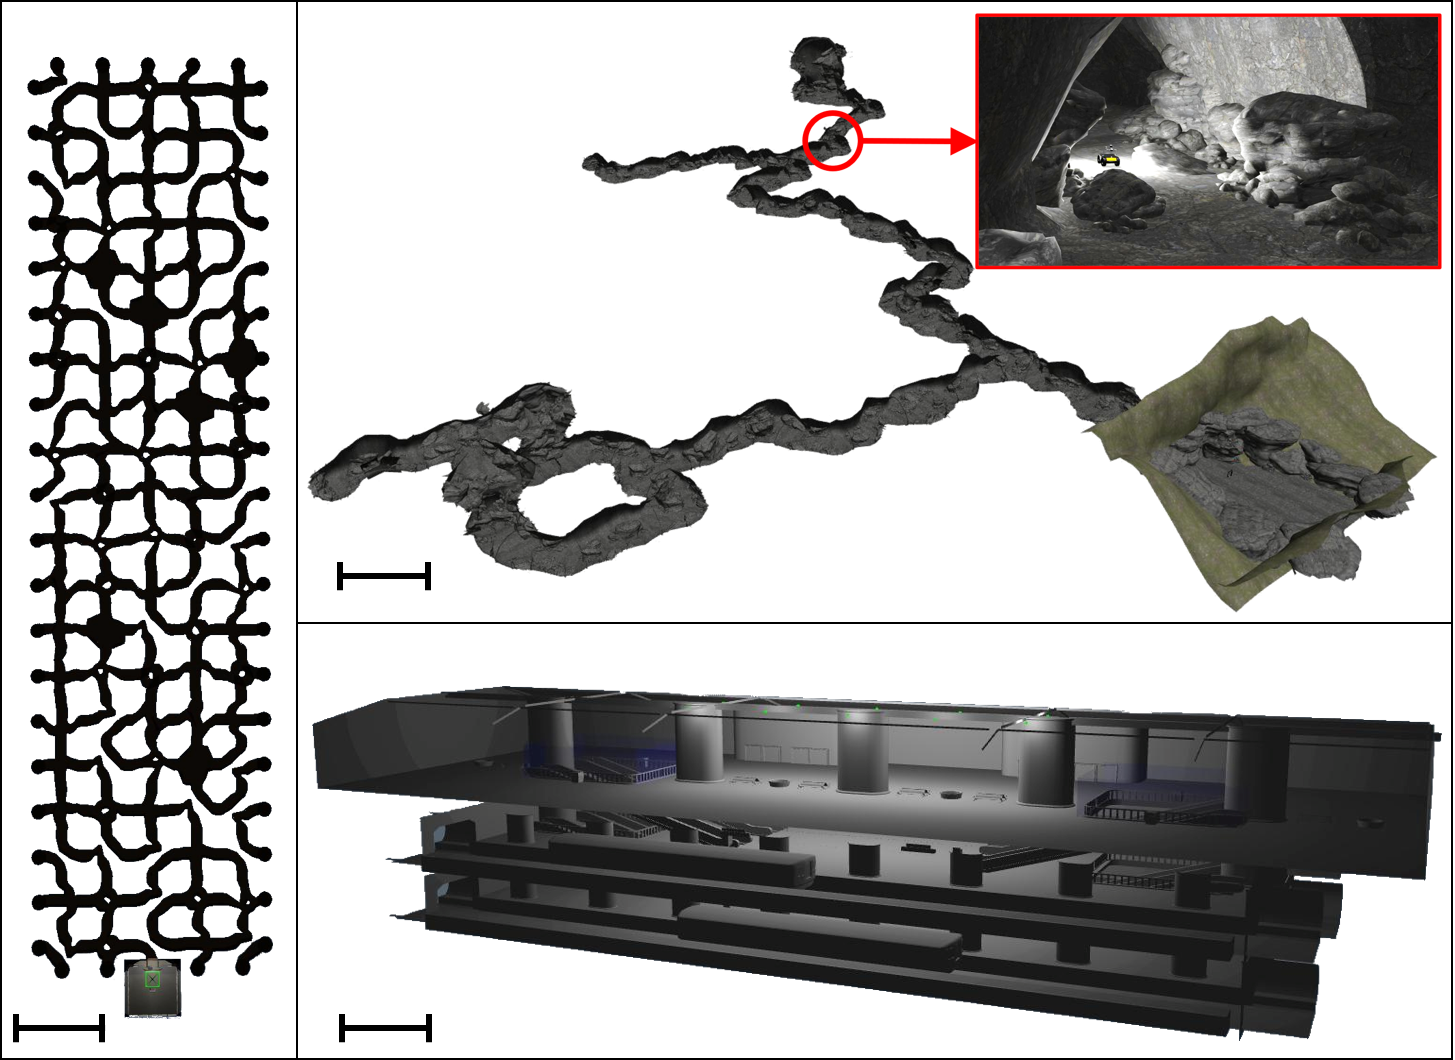
\includegraphics[width=1\columnwidth]{IRM_Planning/figures/combined_gazebo_worlds_V8.png}
% 	%  	}
% 	% %  	\quad
% 	% 	\subfloat[Simulated \\Maze]{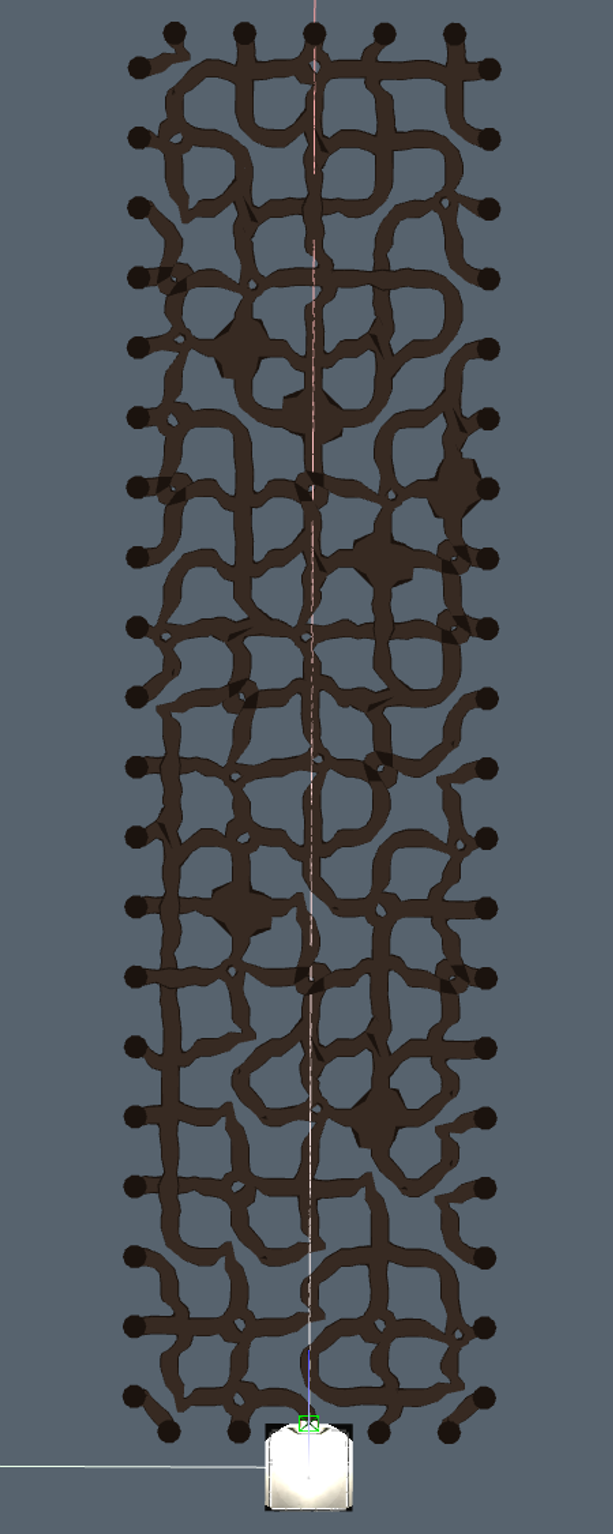
\includegraphics[width=0.3\columnwidth, angle=90]{IRM_Planning/figures/maze.png}}
% 	\caption{Simulated cave (top) and maze (bottom).}
% 	\label{fig:maps_of_cave}
% \end{figure}

% \begin{figure}
% \centering
%     \begin{tikzpicture}
% 	    \node[anchor=south west,inner sep=0] (image) at (0,0) {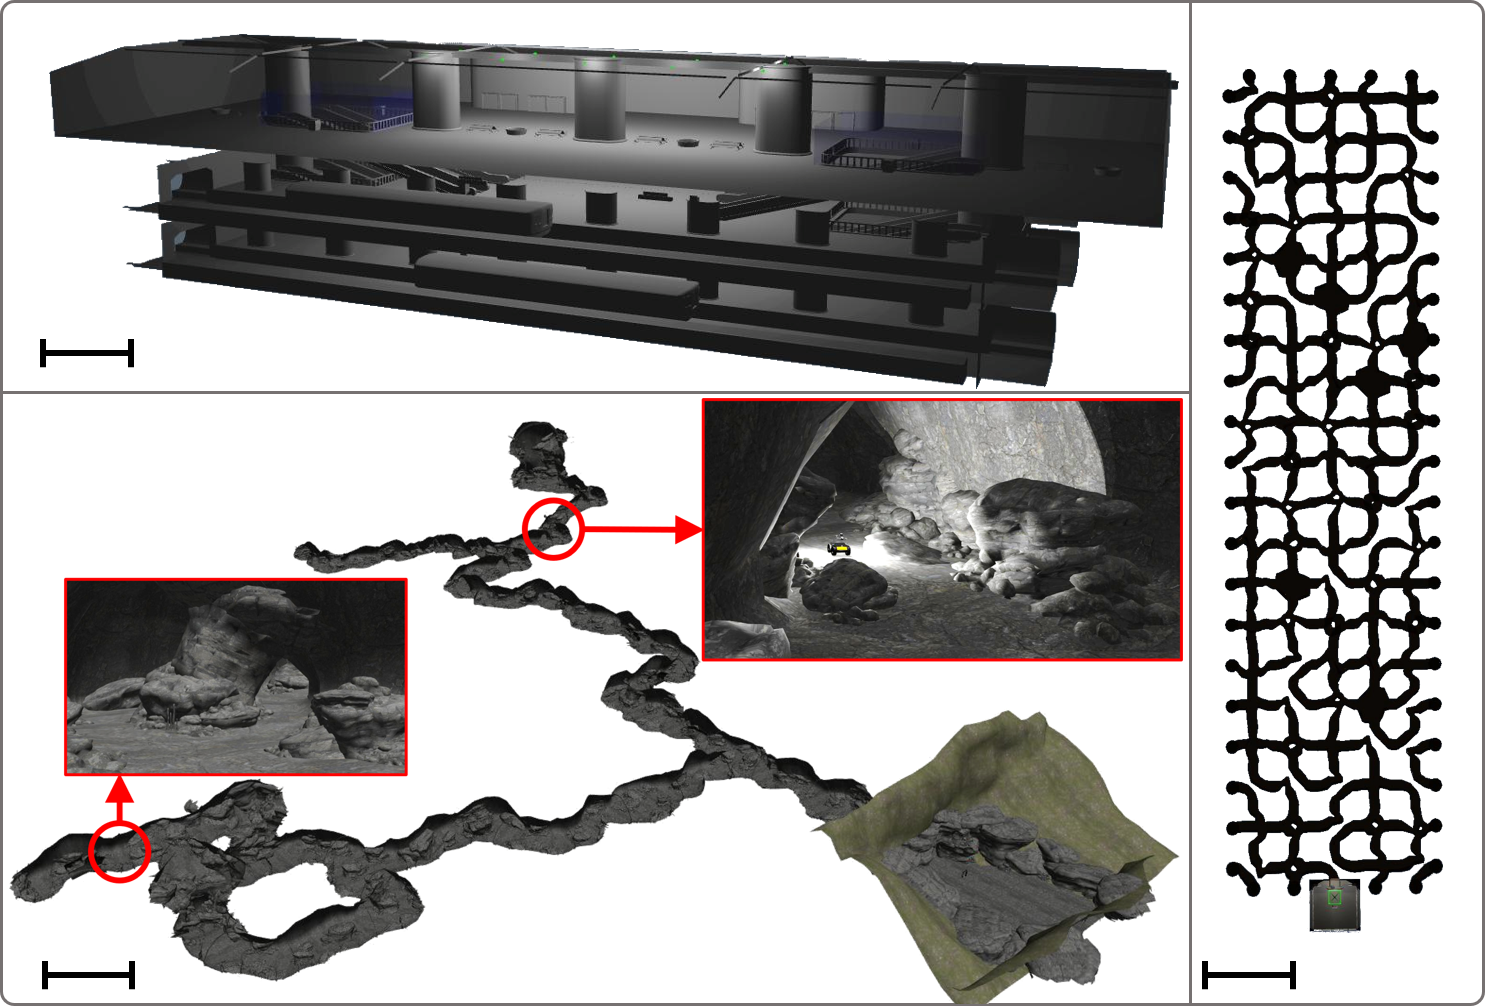
\includegraphics[width=1\columnwidth]{IRM_Planning/figures/combined_gazebo_worlds_V13.png}};
% 	    \begin{scope}[x={(image.south east)},y={(image.north west)}]
	    
% 	    	% Annotations [Letters]
% 	    	\node [above left,align=right,black] at (0.07,0.915) {(a)};
% 	    	\node [above left,align=right,black] at (0.07,0.52) {(b)};
% 	    	\node [above left,align=right,black] at (0.87,0.915) {(c)};
	    	
% 	    	% Annotations [Scale]
% 	    	\node [font=\scriptsize,above left,align=right,black] at (0.115,0.65) {XX m};
% 	    	\node [font=\scriptsize,above left,align=right,black] at (0.115,0.036) {XX m};
% 	    	\node [font=\scriptsize,above left,align=right,black] at (0.89,0.036) {XX m};

% 	    \end{scope}
% 	\end{tikzpicture}	
% \caption{PLGRIM's performance was evaluated in various simulated environments: (a) subway station, (b) cave, and (c) maze.}
% \label{fig:maps_of_cave}
% \end{figure}

% \begin{figure}[h!]
% \centering
%     \begin{tikzpicture}
% 	    \node[anchor=south west,inner sep=0] (image) at (0,0) {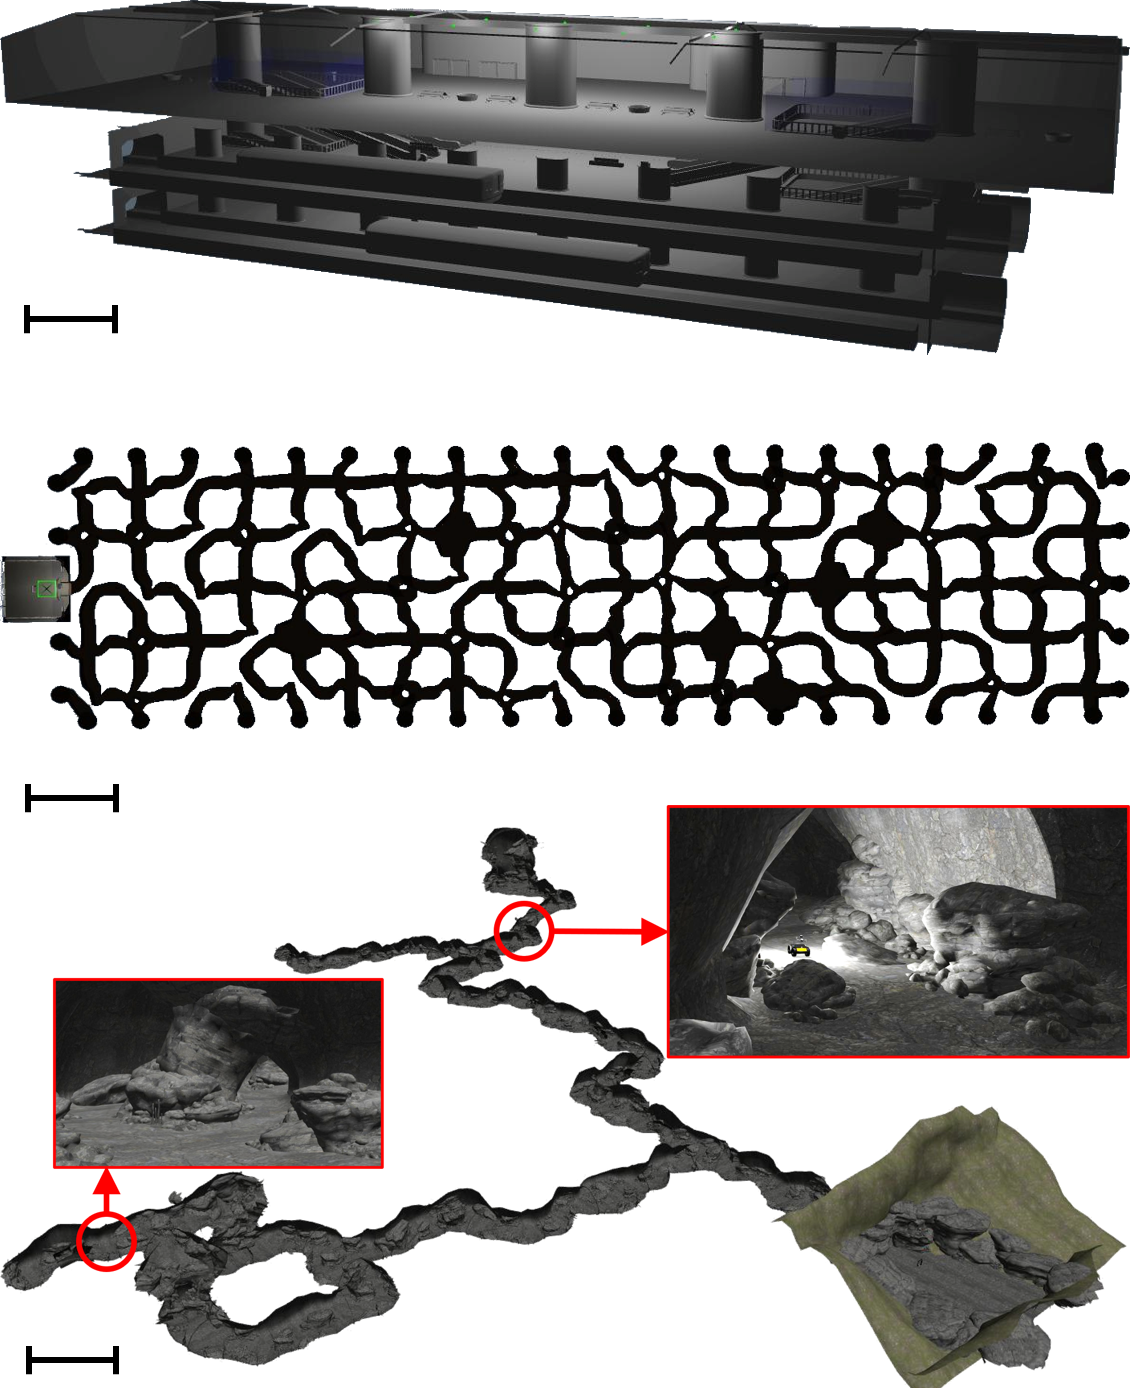
\includegraphics[width=0.85\columnwidth]{IRM_Planning/figures/stacked_sim_worlds.png}};
% 	    \begin{scope}[x={(image.south east)},y={(image.north west)}]
	    
	    
% 	    	% Annotations [Letters]
% 	   % 	\node [above left,align=right,black] at (0.07,0.975) {(a)};
%     	    \node [above left,align=right,black] at (0.35,0.975) {(a) Simulated Subway};
% 	   % 	\node [above left,align=right,black] at (0.07,0.67) {(b)};
%         	\node [above left,align=right,black] at (0.35,0.67) {(b) Simulated Maze};
% 	    	\node [above left,align=right,black] at (0.35,0.35) {(c) Simulated Cave};
	    	
% 	    	% Annotations [Scale]
% 	   % 	\node [font=\scriptsize,above left,align=right,black] at (0.115,0.65) {XX m};
% 	   % 	\node [font=\scriptsize,above left,align=right,black] at (0.115,0.036) {XX m};
% 	   % 	\node [font=\scriptsize,above left,align=right,black] at (0.89,0.036) {XX m};

% 	    \end{scope}
% 	\end{tikzpicture}	
% \caption{PLGRIM's performance was evaluated in various simulated environments: (a) subway station, (b) cave, and (c) maze.}
% \label{fig:maps_of_cave}
% \end{figure}

% font=\fontsize{4pt}{0},

\section{Experimental Results}\label{sec:exp_results}
%\ph{Intro}
In order to evaluate our proposed framework, we perform high-fidelity simulation studies with a four-wheeled vehicle (Husky robot) and real-world experiments with a quadruped (Boston Dynamics Spot robot). Both robots are equipped with custom sensing and computing systems, enabling high levels of autonomy and communication capabilities~\cite{Otsu2020}, (Agha-mohammadi, 2021). The entire autonomy stack runs in real-time on an Intel Core i7 processor with 32 GB of RAM. The stack relies on a multi-sensor fusion framework. The core of this framework is 3D point cloud data provided by LiDAR range sensors mounted on the robots~\cite{Ebadi2020}. We refer to our autonomy stack-integrated Spot as Au-Spot~\cite{AutoSpot}.



\subsection{Baseline Algorithms}
We compare our PLGRIM framework against a local coverage planner baseline (next-best-view method) and a global coverage planner baseline (frontier-based method).
\vspace{-3pt}
\begin{enumerate}[label={\arabic*)}]
  \itemsep0em 
  \setlength{\itemsep}{0pt}
  \setlength{\parskip}{0pt}
  % NBV: (+) locally higher fidelity (small action steps) for evaluation (on high-fidelity local world representation) --> effective local coverage %(while it cannot consider risk/info gain along the path)
  %      (-) no global world representation
  %      (-) sparse policy space (deterministic path to a sampled view-point)
  % HFE: (+) global representation of coverage --> global coverage completeness
  %      (+) Hierarchical FE improves the efficiency to allow local frontier search
  %      (-) sparse world representation (with low-fidelity)
  %      (-) sparse policy space (large action step -- too much of down-sampling, myopic one-step look-ahead -- no further considerations beyond one step)
  \item \textbf{Next-Best-View (NBV)}:
%   NBV is a widely-adopted local coverage planner that returns a path to the best next viewpoint.
% 	Like PLGRIM, it uses an information gain-based reward function, but 
% 	NBV limits its policy search space to the set of shortest paths from the robot to sampled viewpoints within a pre-defined radius.
	NBV first samples viewpoints in a neighborhood of the robot, and then plans a deterministic path over a high-fidelity local world representation to each viewpoint~\cite{bircher2016receding}. The set of viewpoint paths serves as the policy search space. Each policy in the space is evaluated, and NBV selects the policy with the maximum reward, computed using action cost and information gain from the world representation. While NBV is able to leverage local high-fidelity information, it suffers due to its spatially limited world belief and sparse policy space.
% 	The information gain and action cost associated with each path is evaluated using high-fidelity information. 
% 	find the most rewarding path to the viewpoint.  
% 	NBV depends on a lower-level deterministic path planner, 
%   and therefore does not consider a probabilistic understanding of risk and information gain when finding a path to a viewpoint.
  \item \textbf{Hierarchical Frontier-based Exploration (HFE)}:
	Frontier-based exploration methods construct a global, but low-fidelity, representation of the world, where frontiers encode approximate local information gain. The set of frontiers serves as the policy search space. Exploration interleaves a one-step look-ahead frontier selection and the creation of new frontiers, until all frontiers have been explored. Hierarchical approaches can enhance the performance of frontier-based methods by modulating the spatial scope of frontier selection~\cite{umari2017autonomous}. However, while HFE is able to reason across the global world belief, it suffers from downsampling artifacts and a sparse policy space composed of large action steps.
% 	While it can ensure global completeness of exploration, it often suffers from local suboptimality due to its large scale policy space and myopic, one-step look-ahead decision making process.
% 	HFE is an extended version of a frontier-based approach that attempts to mitigate such problems by limiting the spatial scope of frontier selection to a local area.
% 	However, it is still subject to the inherited \textcolor{blue}{(correct term?)} suboptimality due to the low spatial resolution of its policy.
% 	While it can ensure global completeness of exploration, it often suffers from local suboptimality due to its sparse policy space and myopic, one-step look-ahead decision-making process.
% 	HFE is an extended version of a frontier-based approach that attempts to mitigate such problems by limiting the spatial scope of frontier selection to a local area.
% 	However, it is still subject to the inherited \textcolor{blue}{(correct term?)} suboptimality due to the low spatial resolution of its policy.~\cite{umari2017autonomous}
\end{enumerate}
\vspace{-3pt}
Note that in order to achieve reasonable performance in the complex simulated environments, we allow each baseline to leverage our Local and Global IRM structures as the underlying search space.
% , as described in Section~\ref{ssec:belief-managers}.

\begin{figure}[t!]
\centering
    \begin{tikzpicture}
	    \node[anchor=south west,inner sep=0] (image) at (0,0) {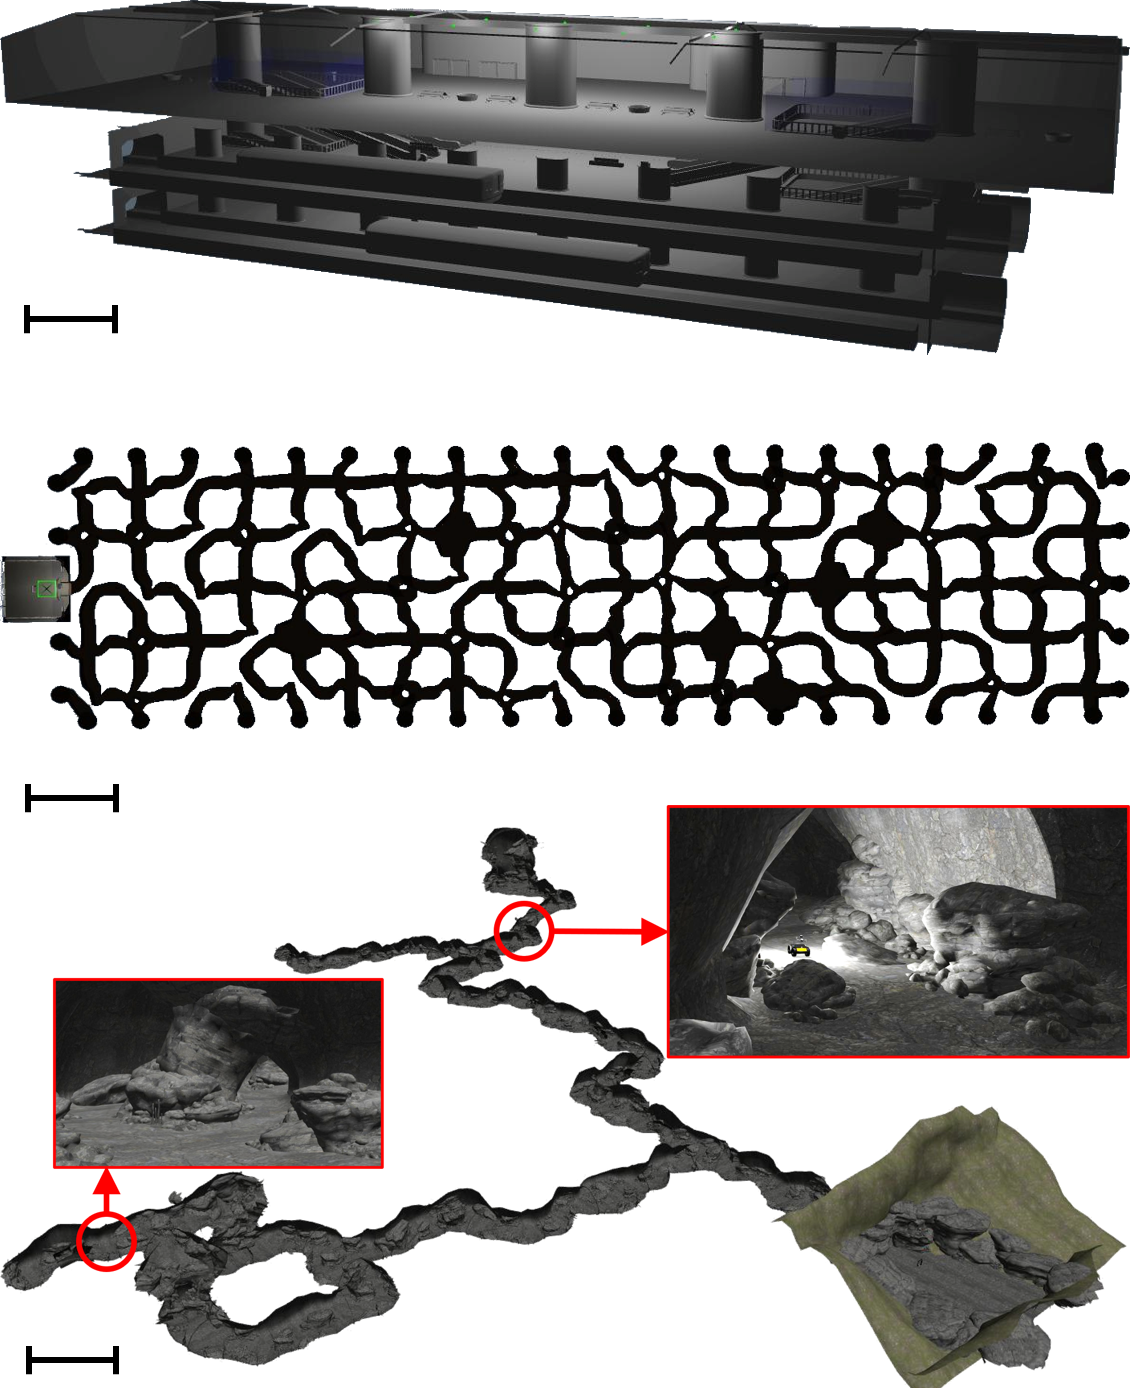
\includegraphics[width=0.85\columnwidth]{IRM_Planning/figures/stacked_sim_worlds.png}};
	    \begin{scope}[x={(image.south east)},y={(image.north west)}]
	    
	    
	    	% Annotations [Letters]
	   % 	\node [above left,align=right,black] at (0.07,0.975) {(a)};
    	    \node [above left,align=right,black] at (0.475,0.99) {(a) Simulated Subway 1x};
	   % 	\node [above left,align=right,black] at (0.07,0.67) {(b)};
        	\node [above left,align=right,black] at (0.37,0.67) {(b) Simulated Maze};
	    	\node [above left,align=right,black] at (0.37,0.33) {(c) Simulated Cave};
	    	
	    	% Annotations [Scale]
	    	\node [font=\scriptsize,above left,align=right,black] at (0.115,0.77) {10 m};
	    	\node [font=\scriptsize,above left,align=right,black] at (0.115,0.425) {50 m};
	    	\node [font=\scriptsize,above left,align=right,black] at (0.115,0.0225) {40 m};

	    \end{scope}
	\end{tikzpicture}	
\caption{PLGRIM's performance was evaluated in various simulated environments: (a) subway station, (b) maze (top-down view), and (c) cave.}
\label{fig:maps_of_cave}
\end{figure}


\begin{figure*}[t!]
    \centering
		\subfloat[][Simulated \\ \; \; \; Subway 1x]{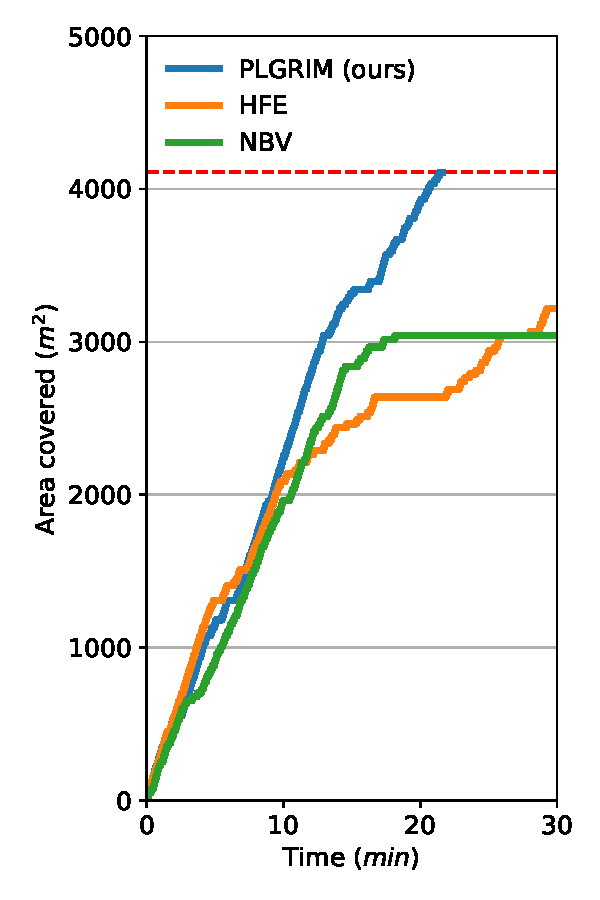
\includegraphics[height=0.5759\columnwidth]{figures/areacov_plots/subway1x.pdf}}
		\subfloat[][Simulated \\ \; \; \; Subway 2x]{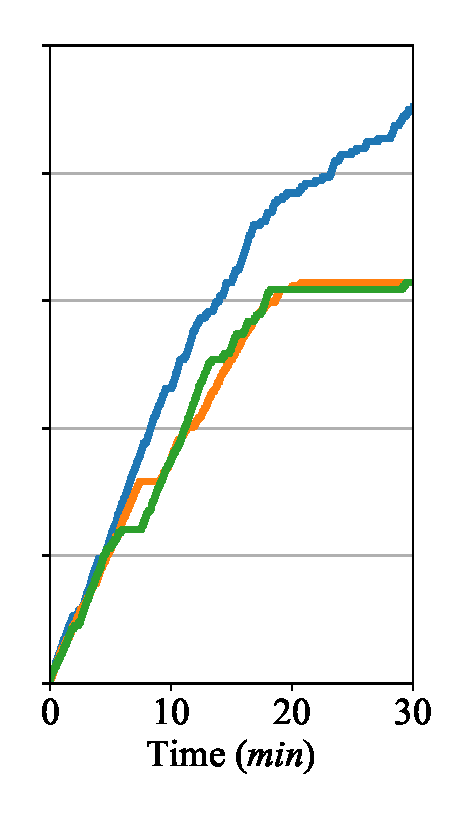
\includegraphics[height=0.57015\columnwidth]{figures/areacov_plots/subway2x.pdf}}	
		\subfloat[][Simulated \\ \; \; \; Subway 3x]{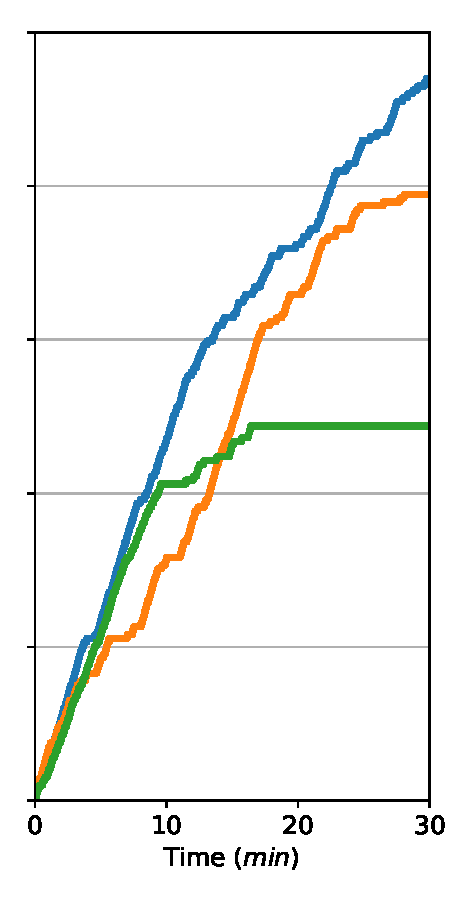
\includegraphics[height=0.57015\columnwidth]{figures/areacov_plots/subway3x.pdf}}	
        \subfloat[][Simulated \\Maze]{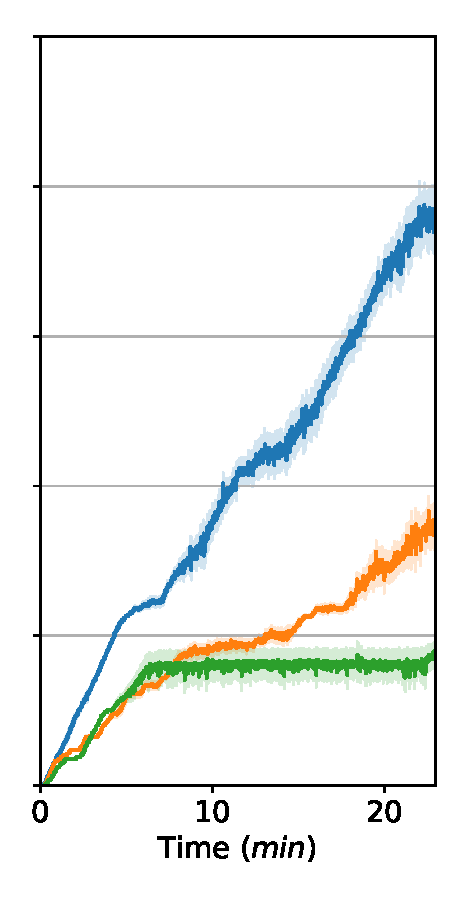
\includegraphics[height=0.57015\columnwidth]{figures/areacov_plots/comparison_cave_cropped.pdf}}
        \subfloat[][Simulated\\Cave]{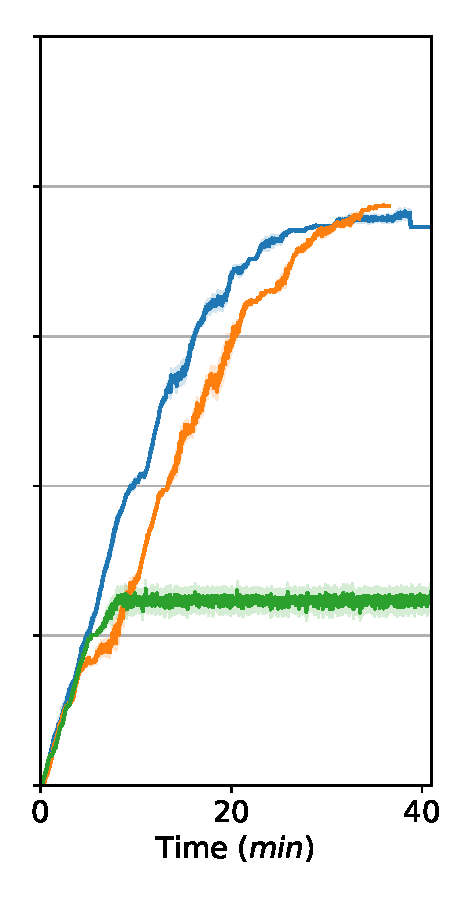
\includegraphics[height=0.57015\columnwidth]{figures/areacov_plots/comparison_simple_cave.pdf}}
		\subfloat[][Real-world \\ \; \; Lava Tube]{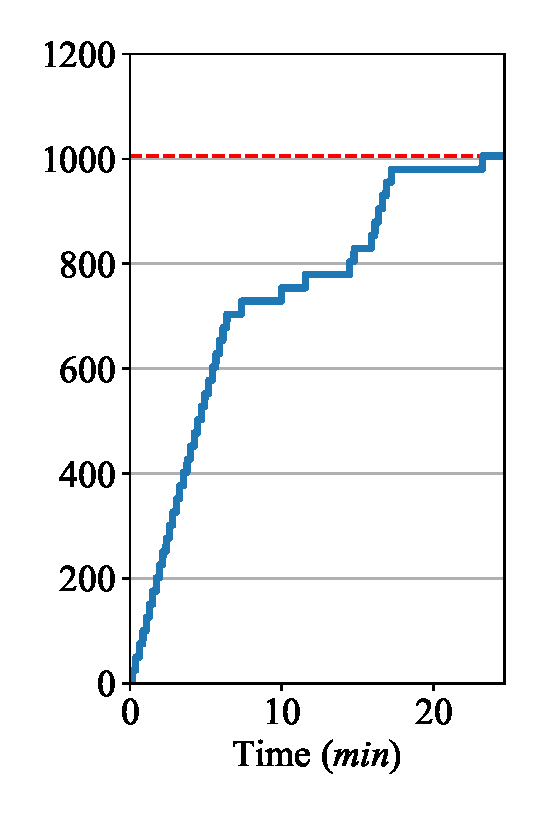
\includegraphics[height=0.5759\columnwidth,clip,trim={20px 0 0 0}]{figures/areacov_plots/lava_tube.pdf}}
		\caption{Exploration by PLGRIM and baseline methods in simulated subway environments of increasing size (a)-(c), and in simulated and real-world cave environments (d)-(f). For (d) and (e), the covered area is the average of two runs. Red dashed lines indicate 100\% coverage of the environments where applicable. In (f), due to the extreme terrain conditions of the lava tube, we restricted Au-Spot's maximum speed to 1~m/s, or half of the platform's manufacturer-specified maximum speed.  
% 		The maximum speed limit of Au-Spot in (f) was set to 50\% of the original limit due to the extremely rough terrain conditions in the lave tube.
		}
    \label{fig:all_together_plot}
\end{figure*}



% \subsection{Test Environments}
% We demonstrate PLGRIM's performance in simulation and on physical robots (see Fig.~\ref{fig:maps_of_cave} and \ref{fig:mlp_hardware_tests}) in:
% \vspace{0pt}
% \begin{enumerate}[label={\arabic*)}]
%   \itemsep0em 
%   \setlength{\itemsep}{0pt}
%   \setlength{\parskip}{0pt}
%   \item \textbf{Simulated Subway Station}: Large interconnected, polygonal rooms with level-floors, which are free of obstacles.
%   \item \textbf{Simulated Cave \& Maze}: Unstructured environments with complex terrain (e.g. rocks, steep slopes) and topology, including narrow passages, dead-ends, open-spaces, and branches with fluctuating curvature. 
%   \item \textbf{Real-world Lava Tube}: Located in Lava Beds National Monument, Tulelake, CA. The cave consists of a main lava tube and a series of smaller, auxiliary tubes branching off. The floor is composed of undulating smooth and ropy masses of cooled lava. Some areas of the floor are covered by large boulders, due to ceiling breakdown.
% \end{enumerate}
% \vspace{-4pt}


\subsection{Simulation Evaluation}
We demonstrate PLGRIM's performance, as well as that of the baseline algorithms, in a simulated subway, maze, and cave environment. Fig.~\ref{fig:maps_of_cave} visualizes these environments.
% We demonstrate PLGRIM's performance in the following simulated worlds:
% \vspace{0pt}
% \begin{enumerate}[label={\arabic*)}]
% %   \itemsep5em 
%   \setlength{\itemsep}{0pt}
%   \setlength{\parskip}{0pt}
%   \item \textbf{Subway Station}: Large interconnected, polygonal rooms with level-floors, which are free of obstacles (Fig.~\ref{fig:maps_of_cave}(a)). 
%   \item \textbf{Cave \& Maze}: Unstructured environments with complex terrain (e.g. rocks, steep slopes) and topology, including narrow passages, dead-ends, open-spaces, and branches with fluctuating curvature (Fig.~\ref{fig:maps_of_cave}(b)-(c)). 
% \end{enumerate}
% \vspace{-3pt}
% \noindent

% \vspace{-2.5pt}
\subsubsection{Simulated Subway Station:} \hfill
\vspace{-0.25pt}

\noindent
The subway station consists of large interconnected, polygonal rooms with smooth floors, devoid of obstacles. There are three varying sized subway environments, whose scales are denoted by 1x, 2x, and 3x. 
Fig.~\ref{fig:all_together_plot}(a)-(c) shows the scalable performance of PLGRIM against the baselines. 
In a relatively small environment without complex features (Subway 1x), NBV performance is competitive as it evaluates high-resolution paths based on information gain.
However, as the environment scale grows, its myopic planning easily gets \textit{stuck} and the robot's coverage rate drops significantly. 
HFE shows inconsistent performance in the subway environments. The accumulation of locally suboptimal decisions, due to its sparse environment representation, leads to the construction of a globally inefficient IRM structure. As a result, the robot must perform time-consuming detours in order to \textit{pick up} leftover frontiers.  
% Hence, HFE's local exploration is highly susceptible to the  Global IRM
% which results in suboptimal decisions. 

% Its global planning policy relies on frontier selection. Thus, in a wide-open environment, its decision-making is often suboptimal.
%
\subsubsection{Simulated Maze and Cave:} \hfill
\vspace{-0.25pt}

\noindent
The maze and cave are both unstructured environments with complex terrain (rocks, steep slopes, etc.) and topology (narrow passages, sharp bends, dead-ends, open-spaces, etc.).
The coverage rates for each algorithm are displayed in Fig.~\ref{fig:all_together_plot}(d)-(e). 
%
PLGRIM outperforms the baseline methods in these environments. By constructing long-horizon coverage paths over a high-resolution world belief representation,
% PLGRIM is able to guide the robot through hazardous terrain. 
PLGRIM enables the robot to safely explore through hazardous terrain. 
Simultaneously, it maintains an understanding of the global world, which is leveraged when deciding where to explore next after exhausting all local information.
% uidance according to its global world belief. 
% due to its hierarchical belief and policy decomposition, 
% leading to a dense local coverage planning and large-scale global guidance.
%
In the cave, NBV's reliance on a deterministic path, without consideration of probabilistic risk, causes the robot to drive into a pile of rocks and become inoperable. NBV exhibits similarly poor performance in the maze. However, in this case, NBV's myopic planning is particularly ineffectual when faced with navigating a topologically-complex space, and the robot ultimately gets \textit{stuck}.   
% In the maze environment, NBV's The complex topology of the maze environment myopic path planning get stuck. 
% causes the robot to get stuck in boulders 
% explores well until hitting a dead-end; due to lack of global-scale guidance
%
As was the case in the subway, HFE suffers in the topologically-complex maze due to an accumulation of suboptimal local decisions. In particular, frontiers are sometimes not detected in the sharp bends of the maze, leaving the robot with an empty local policy space. As a result, the robot cannot progress and must spend considerable time backtracking along the IRM to distant frontiers.  
% --while it performs well in the cave, it suffers in the topologically-complex maze. 
% HFE performs well in the cave with relatively simple topology, but performs poorly in the maze.
% This is due to the fact that frontier-based exploration has a sparse action space, which is intrinsically brittle, especially in narrow passages or sharp corners of the maze environment.

% Since HFE's decision making is based on one-step look-ahead myopic planning, its performance is significantly challenged given a complex topology.


% \begin{figure}[h!]
% \centering
%     \begin{tikzpicture}
% 	    \node[anchor=south west,inner sep=0] (image) at (0,0) {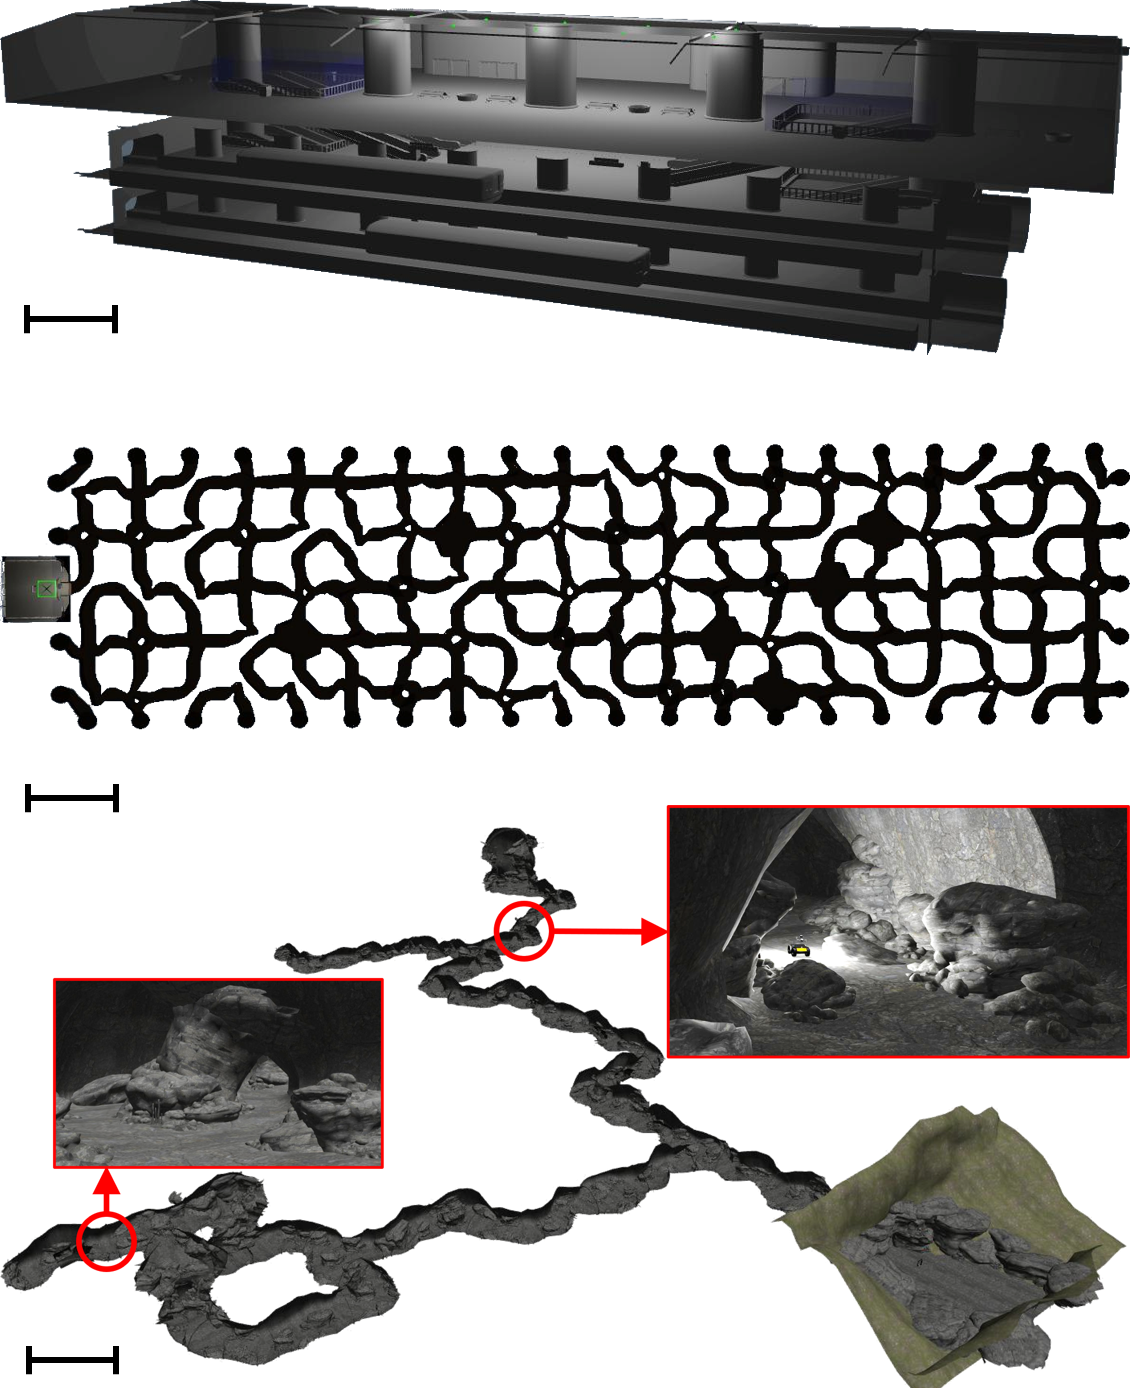
\includegraphics[width=0.85\columnwidth]{IRM_Planning/figures/stacked_sim_worlds.png}};
% 	    \begin{scope}[x={(image.south east)},y={(image.north west)}]
	    
	    
% 	    	% Annotations [Letters]
% 	   % 	\node [above left,align=right,black] at (0.07,0.975) {(a)};
%     	    \node [above left,align=right,black] at (0.475,0.99) {(a) Simulated Subway 1x};
% 	   % 	\node [above left,align=right,black] at (0.07,0.67) {(b)};
%         	\node [above left,align=right,black] at (0.37,0.67) {(b) Simulated Maze};
% 	    	\node [above left,align=right,black] at (0.37,0.33) {(c) Simulated Cave};
	    	
% 	    	% Annotations [Scale]
% 	    	\node [font=\scriptsize,above left,align=right,black] at (0.11,0.765) {1  0 m};
% 	    	\node [font=\scriptsize,above left,align=right,black] at (0.115,0.425) {50 m};
% 	    	\node [font=\scriptsize,above left,align=right,black] at (0.115,0.0225) {40 m};

% 	    \end{scope}
% 	\end{tikzpicture}	
% \caption{PLGRIM's performance was evaluated in various simulated environments: (a) subway station, (b) maze (top-down view), and (c) cave.}
% \label{fig:maps_of_cave}
% \end{figure}

\begin{figure*}[h!]
\centering
    \begin{tikzpicture}
	    \node[anchor=south west,inner sep=0] (image) at (0,0) {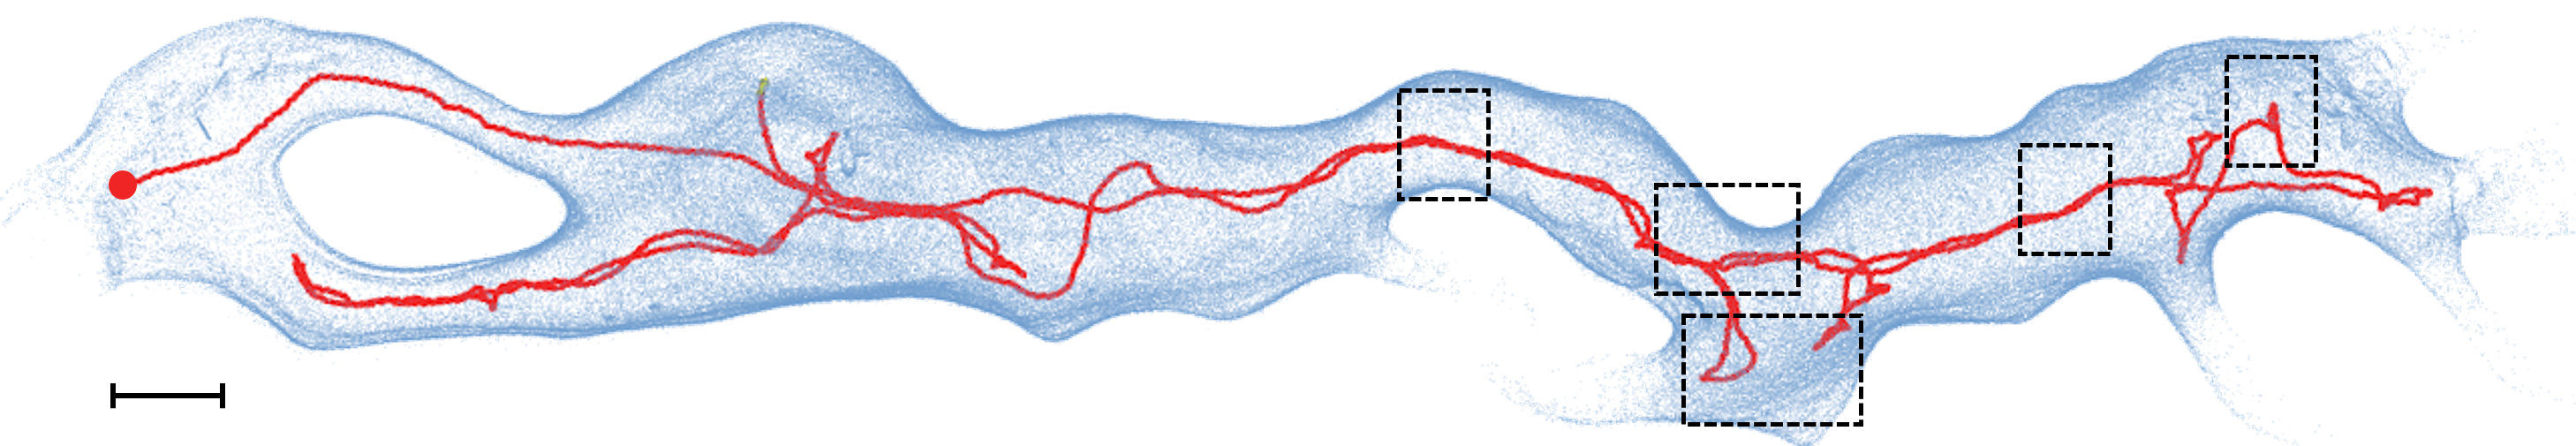
\includegraphics[width=1\textwidth]{figures/point_cloud_lava_tube_labels_v7.png}};
	    \begin{scope}[x={(image.south east)},y={(image.north west)}]
	    
	    	% Annotations [Letters]
	    	\node [above left,align=right,black] at (0.575,0.422) {H};
	    	\node [above left,align=right,black] at (0.7,0.56) {A-C};
	    	\node [above left,align=right,black] at (0.765,0.07) {F-G};
	    	\node [above left,align=right,black] at (0.815,0.295) {D};
	    	\node [above left,align=right,black] at (0.895,0.855) {E};
	    	
	    	\node [font=\scriptsize, above left,align=right,black] at (0.0855,0.12) {4 m};
	    	
	    \end{scope}
	\end{tikzpicture}
	\caption{PLGRIM's exploration trajectory in Valentine Cave, Lava Beds National Monument, Tulelake, CA. Exploration started at the mouth of the cave (red circle), reached the end of the cave on the right, and returned back to visit uncovered areas. Boxes indicate the portions of the trajectory associated with alphabetized snapshots from Fig.~\ref{fig:mlp_hardware_tests} and Fig.~\ref{fig:glp_hardware_tests}.
	}
    \label{fig:lava_tube_traj}
\end{figure*}

% \vspace{-200pt}

\begin{figure*}[h!]
\centering
    \begin{tikzpicture}
	   % \node[anchor=south west,inner sep=0] (image) at (0,0) {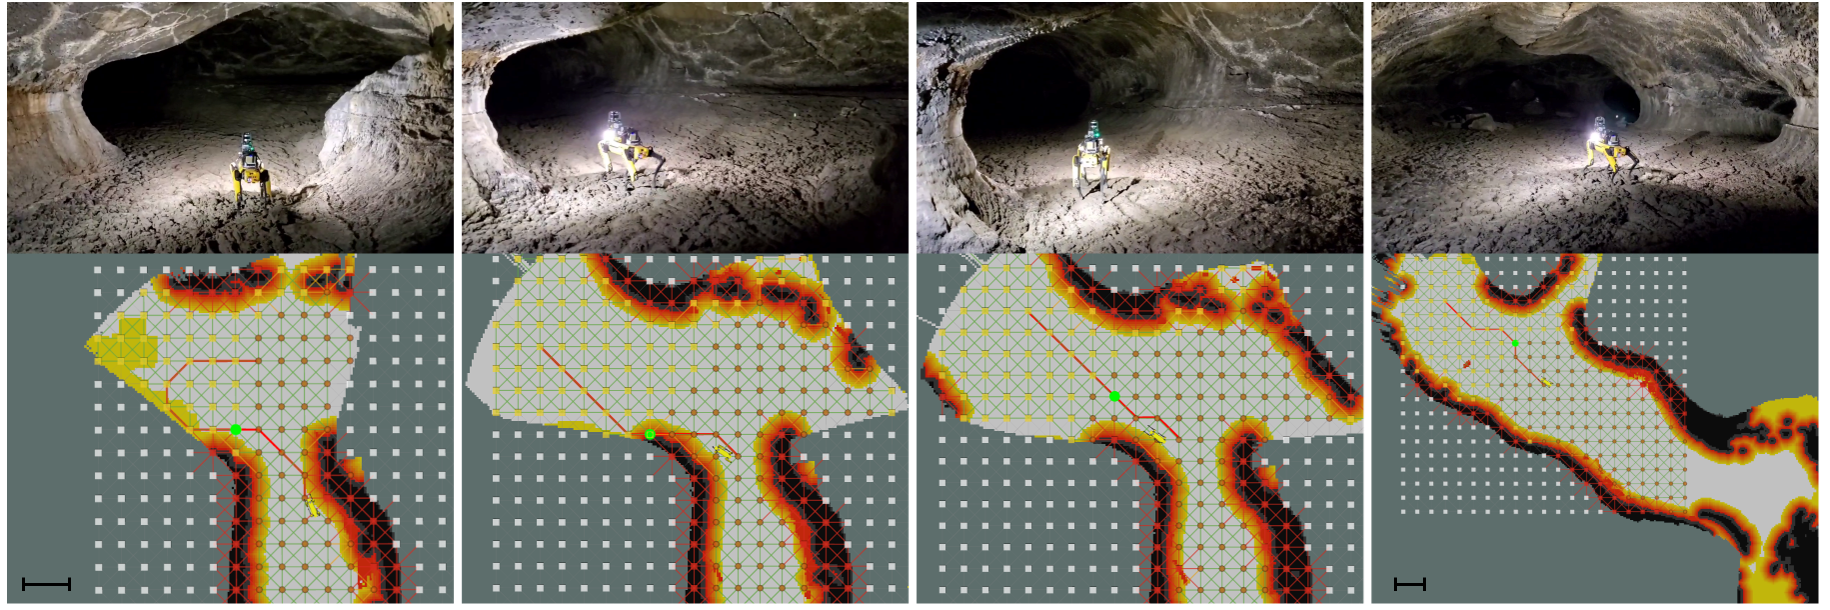
\includegraphics[width=1\textwidth]{figures/mlp_figure_scale.png}};
       \node[anchor=south west,inner sep=0] (image) at (0,0) {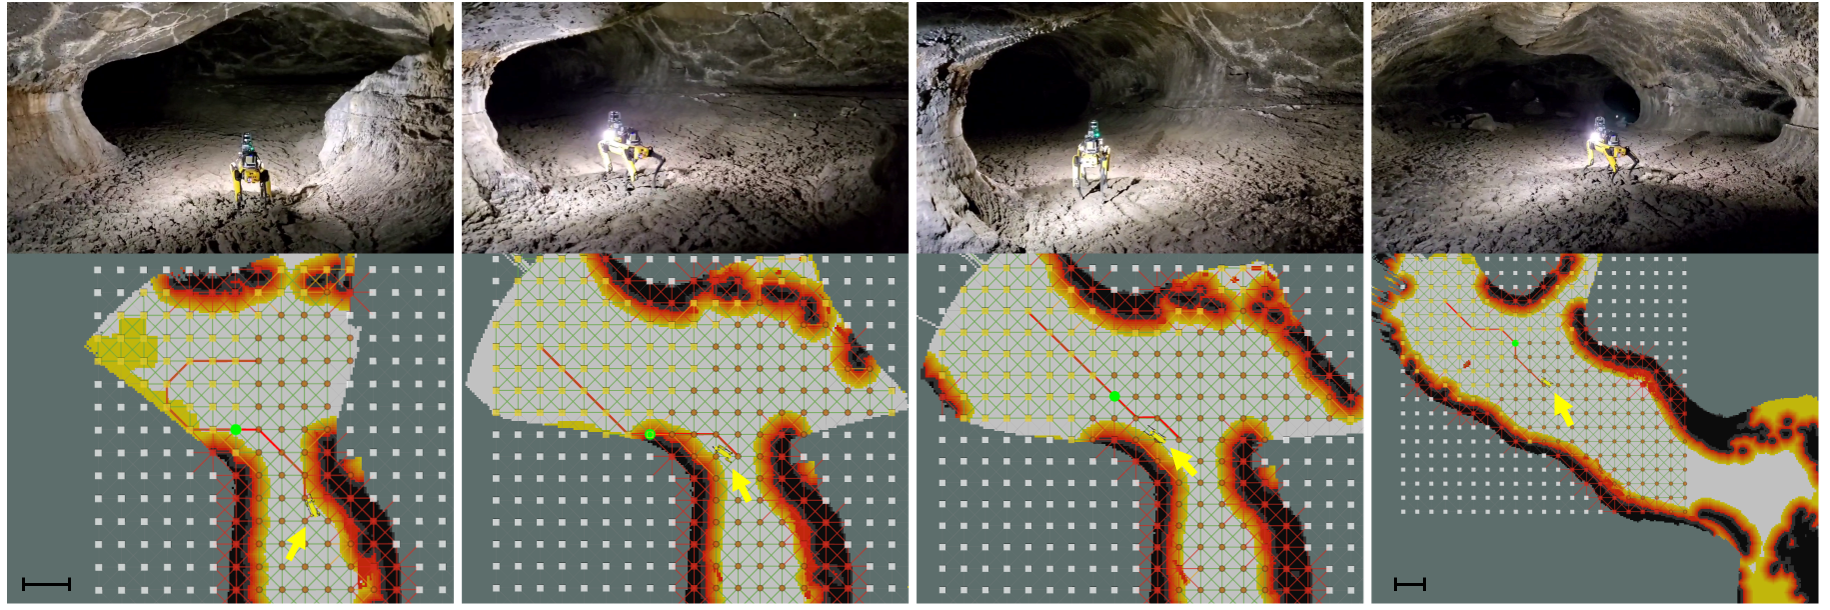
\includegraphics[width=1\textwidth]{IRM_Planning/figures/mlp_hardware_scale_arrows.png}};
	    \begin{scope}[x={(image.south east)},y={(image.north west)}]
	    
	    	% Annotations [Letters]
	    	\node [above left,align=right,white] at (0.035,0.91) {\textbf{A}};
	    	\node [above left,align=right,white] at (0.28,0.91) {\textbf{B}};
	    	\node [above left,align=right,white] at (0.53,0.91) {\textbf{C}};
	    	\node [above left,align=right,white] at (0.78,0.91) {\textbf{D}};
	    
	    	% Annotations [Time]
	    	\node [font=\scriptsize,above left,align=right,white] at (0.245,0.58) {\textbf{t=5:08}};
	    	\node [font=\scriptsize,above left,align=right,white] at (0.495,0.58) {\textbf{t=5:20}};
	    	\node [font=\scriptsize,above left,align=right,white] at (0.742,0.58) {\textbf{t=5:24}};
	    	\node [font=\scriptsize,above left,align=right,white] at (.992,0.58) {\textbf{t=6:24}};
	    	
	    	% Annotations [Scale]
	    	\node [font=\scriptsize,above left,align=right,black] at (0.044,0.045) {2 m};
	    	\node [font=\scriptsize,above left,align=right,black] at (0.787,0.045) {2 m};

	    \end{scope}
	\end{tikzpicture}	
\caption{The Local IRM (yellow, brown, and white nodes represent uncovered, covered and unknown areas, respectively) is shown overlaid on the Riskmap. A yellow arrow indicates the robot's location. LCP plans a path (red) that fully covers the local area (snapshot A). When $p(W^\ell)$ updates, the path is adjusted to extend towards the large uncovered swath while maintaining smoothness with the previous path. Another $p(W^\ell)$ update reveals that the path has entered a hazardous area---wall of lava tube (snapshot B). As a demonstration of LCP's resiliency, the path shifts away from the hazardous area, and the robot is re-directed towards the center of the tube (snapshot C). One minute later, the robot encounters a fork in the cave. The LCP path curves slightly toward fork apex (for maximal information gain) before entering the wider, less-risky channel (snapshot D). } 
\label{fig:mlp_hardware_tests} 
\end{figure*}

% \begin{figure*}[h!]
% \centering
%     \begin{tikzpicture}
% 	    \node[anchor=south west,inner sep=0] (image) at (0,0) {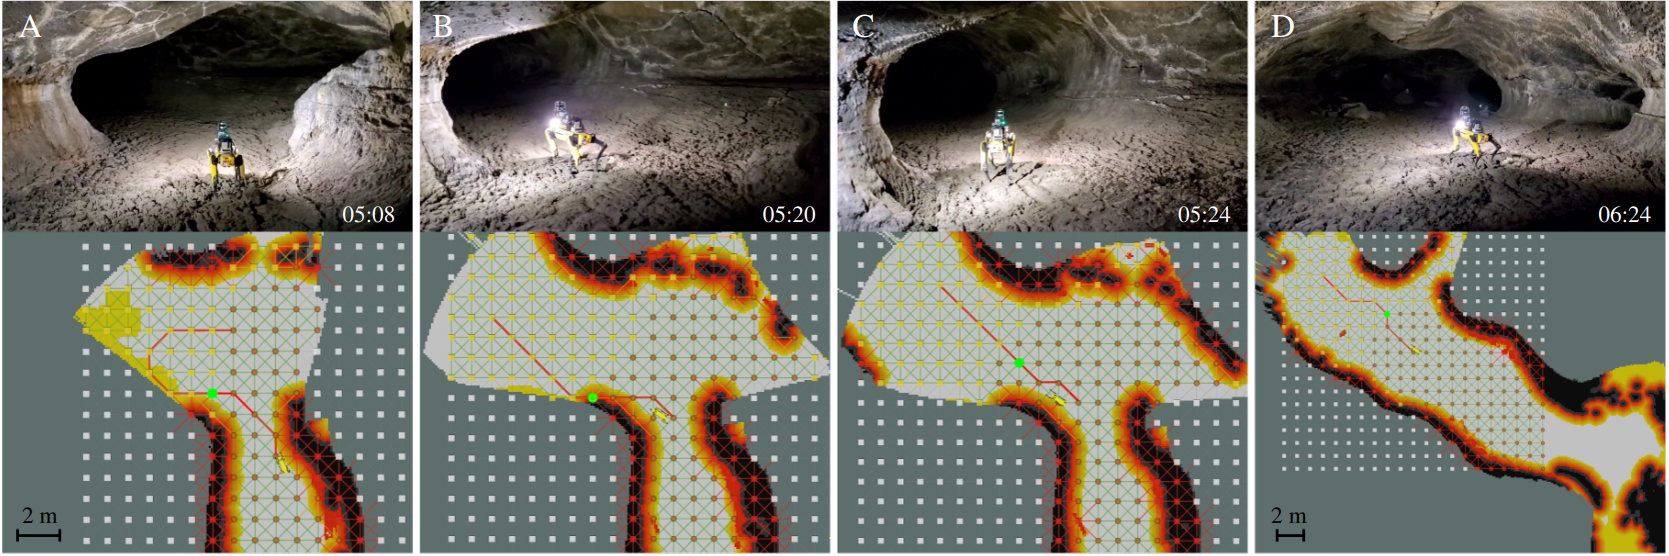
\includegraphics[width=.75\textwidth]{figures/MLP_screenshot.png}};
% 	\end{tikzpicture}		
% \caption{LCP plans looping path that fully covers area represented by Local IRM (snapshot A). Path is updated to extend towards large uncovered swath while maintaining consistency with prior path. Riskmap update reveals that path has entered a hazardous area---wall of lava tube (snapshot B). As a demonstration of LCP's resilience, path shifts away from hazardous area and robot is re-directed towards center of tube (snapshot C). One minute later, robot encounters fork in cave system. LCP path curves slightly toward fork apex before entering larger, less-risky channel (snapshot D). } \label{fig:mlp_hardware_tests} 
% \end{figure*}


\begin{figure*}[h!]
\centering
    \begin{tikzpicture}
	    \node[anchor=south west,inner sep=0] (image) at (0,0) {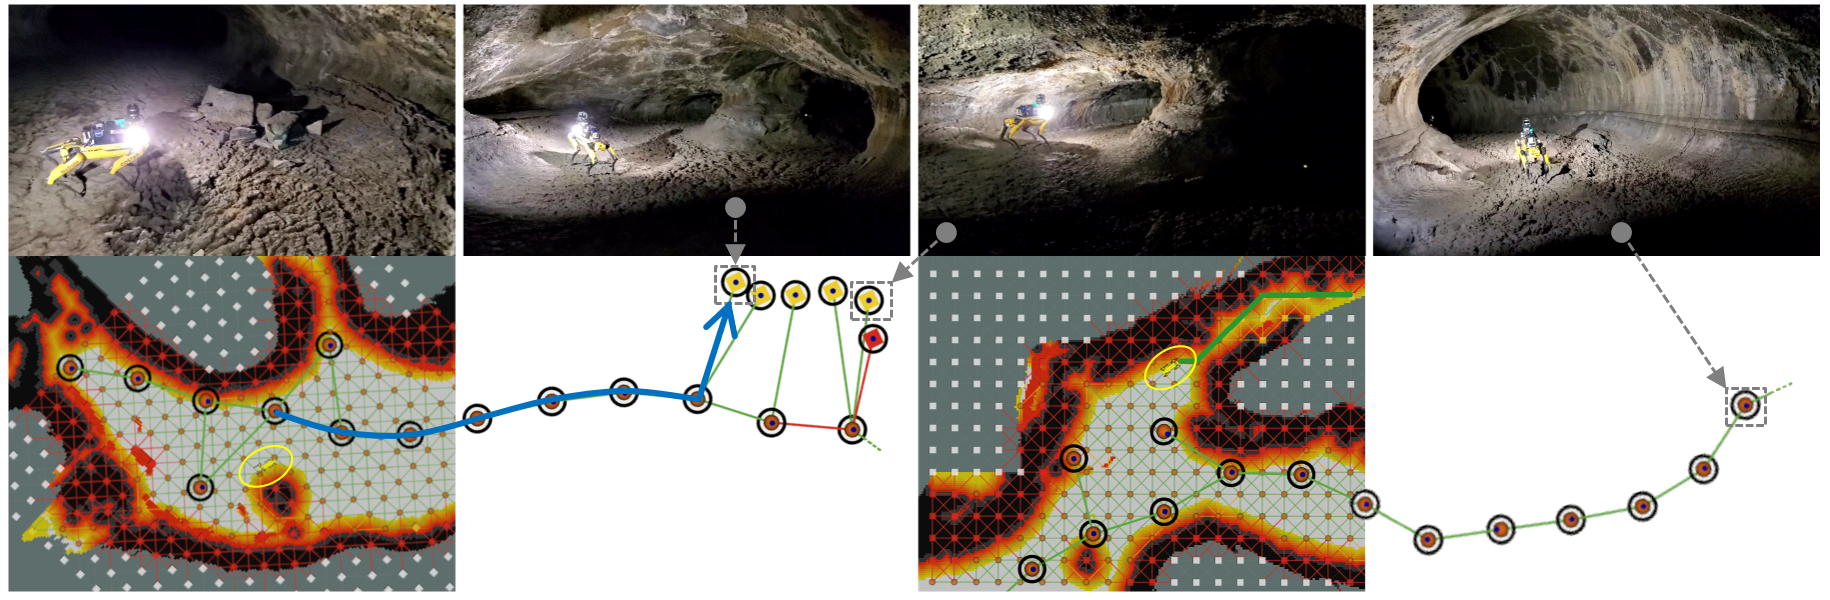
\includegraphics[width=1\textwidth]{IRM_Planning/figures/glp_figure_processed_shift.png}};
	    \begin{scope}[x={(image.south east)},y={(image.north west)}]
	    
	    	% Annotations [Letters]
	    	\node [above left,align=right,white] at (0.035,0.91) {\textbf{E}};
	    	\node [above left,align=right,white] at (0.28,0.91) {\textbf{F}};
	    	\node [above left,align=right,white] at (0.53,0.91) {\textbf{G}};
	    	\node [above left,align=right,white] at (0.78,0.91) {\textbf{H}};
	    	
	    	% Annotations [Time]
	    	\node [font=\scriptsize,above left,align=right,white] at (0.245,0.58) {\textbf{t=09:11}};
	    	\node [font=\scriptsize,above left,align=right,white] at (0.495,0.58) {\textbf{t=10:36}};
	    	\node [font=\scriptsize,above left,align=right,white] at (0.742,0.58) {\textbf{t=12:26}};
	    	\node [font=\scriptsize,above left,align=right,white] at (.992,0.58) {\textbf{t=14:16}};
	    	

	    \end{scope}
	\end{tikzpicture}	
\caption{Portions of the Global IRM constructed in the lava tube are visualized--yellow nodes represent frontiers, brown nodes represent breadcrumbs. Gray arrows associate a frontier with a snapshot of the robot exploring that frontier. GCP plans a path (blue) along the Global IRM to a target frontier after the local area is fully covered (snapshot E). The robot explores the area around the frontier (snapshot F), and then explores a neighboring frontier at the opening of a narrow channel to it's right. LCP plans a path (green) into the channel (snapshot G). Later, after all local areas have been explored, the robot is guided back towards the mouth of cave along the breadcrumb nodes (snapshot H).} \label{fig:glp_hardware_tests} 
\end{figure*}

% \begin{figure*}[h!]
% \centering
%     \begin{tikzpicture}
% 	    \node[anchor=south west,inner sep=0] (image) at (0,0) {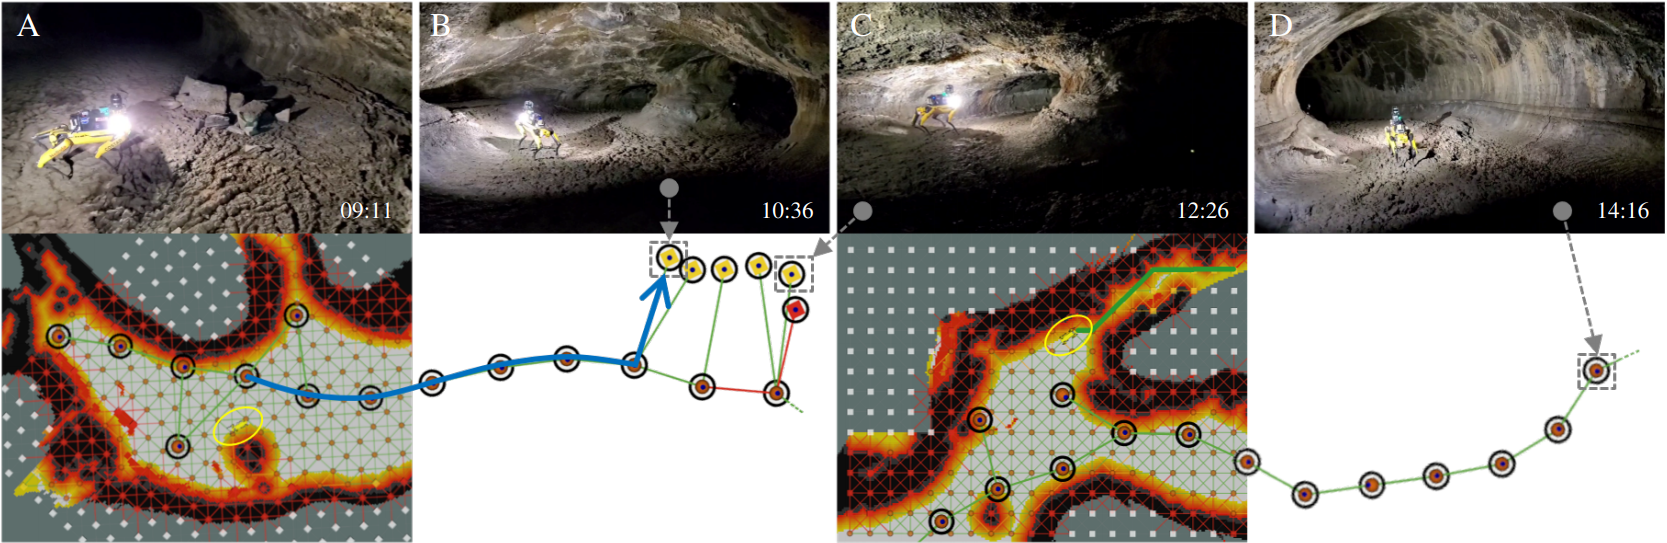
\includegraphics[width=0.75\textwidth]{figures/GLP_screenshot.png}};
% 	\end{tikzpicture}	
% \caption{GCP plans path (blue) along Global IRM to frontier after local area is fully covered (snapshot A). Robot explores area around frontier (snapshot B), and then explores neighboring frontier at opening of side channel. LCP plans path (green) into channel (snapshot C). Later, after all local area has been explored, GCP guides robot back towards mouth of cave (snapshot D).} \label{fig:glp_hardware_tests} 
% \end{figure*}



% \begin{figure}
%      \centering
%   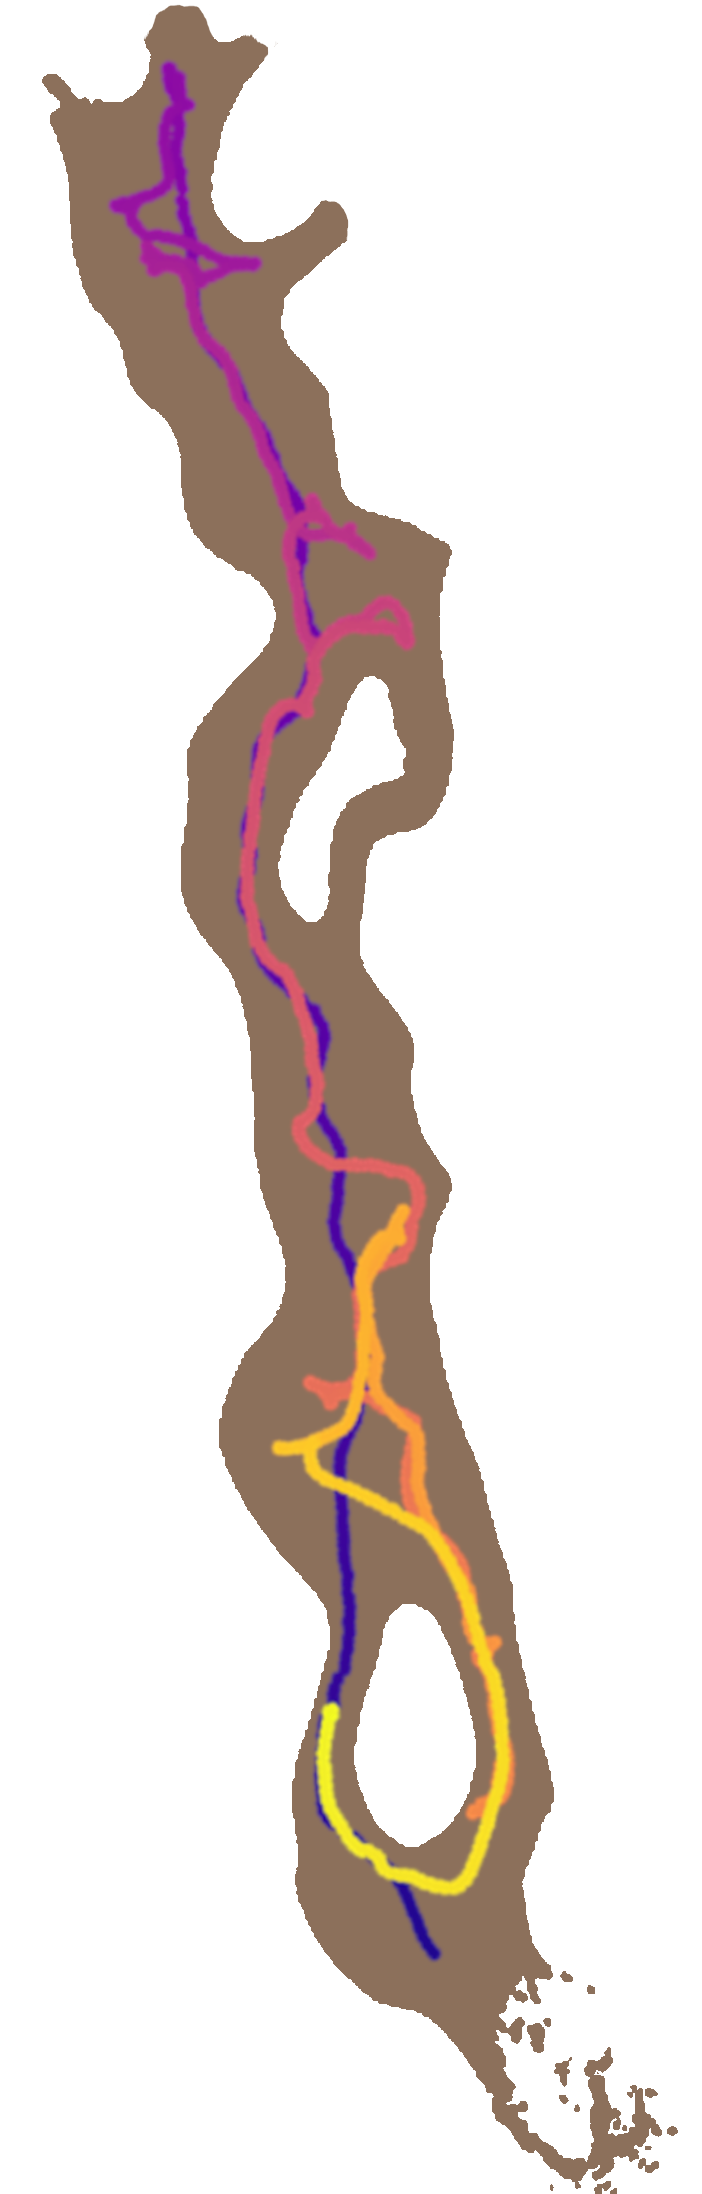
\includegraphics[width=0.45\columnwidth,angle=90, scale=0.7
%   ]{figures/darpa_tv_test_figs/cave_path_overlay_lightbrown.png}%
% 	% \caption{Robot trajectory on cave profile from hardware test.}
% 	\caption{Au-Spot's autonomous exploration trajectory from the field test in Valentine Cave in Lava Beds National Monument, Tulelake, CA. \note{Add a scale on this figure as well?}}
%     \label{fig:lava_tube_traj}
% \end{figure}


\subsection{Real-World Evaluation}
We extensively validated PLGRIM on physical robots in real-world environments. In particular, PLGRIM was run on Au-Spot in a lava tube, located in Lava Beds National Monument, Tulelake, CA. The cave consists of a main tube, which branches into smaller, auxiliary tubes. The floor is characterized by ropy masses of cooled lava. Large boulders, from ceiling breakdown, are scattered throughout the tube.
Fig.~\ref{fig:lava_tube_traj} shows the robot's trajectory overlaid on the aggregated LiDAR point cloud.
Fig.~\ref{fig:mlp_hardware_tests} and \ref{fig:glp_hardware_tests} discuss how PLGRIM is able to overcome the challenges posed by large-scale environments with complex terrain and efficiently guide the robot's exploration. Fig.~\ref{fig:all_together_plot}(f) shows the area covered over time.



%%%%%%%%%%%%%%%%%%%%%%%%%%%%%%%%%%%%%%%%%%%%%%%%%%%%%%%%%%%%%%%%%%%%%%%%%%%%%%%%
\section{Conclusion}\label{sec:conclusion}
In this work, we develop a hierarchical framework for exploring large-scale, unknown environments with complex terrain in a POMDP setting. 
% To obtain a tractable solution, we discretize the belief space into a robot and task-relevant graph structure. 
To obtain a tractable solution, we introduce a hierarchical belief space representation that effectively encodes a large-scale world state, while simultaneously capturing high-fidelity information local to the robot. Then we propose cascaded POMDP solvers that reason over long horizons within a suitable replanning time. 
% This simplifies the planning problem and reduces our search space for good policies.
% The hierarchical planning framework and formalization of the unified optimal policy allows us to solve the coverage planning problem in large-scale environments with rugged terrain.
We demonstrate our framework in high-fidelity dynamic simulation environments and in real-world environments, namely a natural cave.  
% Future work includes learning-based methods for graph expansion information gain estimation, and a richer incorporation of risk and time into the graph planning framework.
%
% Future work includes using learning-based methods for estimating graph expansion information gain, and 
% incorporating richer  of risk and time into the graph planning framework.
Future work includes incorporating semantic information gain in IRMs, such as science target signature,
and extending this framework to multi-robot coverage problems.
% Another interesting extension of this framework is to multi-robot coverage problems.

\vspace{-10pt}

\section*{Acknowledgment}
% The work is partially supported by the Jet Propulsion Laboratory, California Institute of Technology, under a contract with the National Aeronautics and Space Administration (80NM0018D0004), and Defense Advanced Research Projects Agency (DARPA).
% We acknowledge Dr. Jennifer Blank at NASA Ames Research Center and
% the BRAILLE Mars Analog project funded by the NASA PSTAR program NNH16ZDA001N.
% We also acknowledge the Resource Staff at Lava Beds National Monument for support of our field efforts.
The work is partially supported by the Jet Propulsion Laboratory, California Institute of Technology, under a contract with the National Aeronautics and Space Administration (80NM0018D0004), Defense Advanced Research Projects Agency (DARPA), and the BRAILLE Mars Analog project funded by the NASA PSTAR program (NNH16ZDA001N).
We acknowledge our team members in Team CoSTAR for the DARPA Subterranean Challenge, Dr. Jennifer Blank at NASA Ames Research Center, Shushman Choudhury, and the resource staff at Lava Beds National Monument for support of our field efforts.
\vspace{-10pt}


%%%%%%%%%%%%%%%%%%%%%%%%%%%%%%%%%%%%%%%%%%%%%%%%%%%%%%%%%%%%%%%%%%%%%%%%%%%%%%%%
% \bibliographystyle{aaai21}  % redundant
\bibliography{references}  % .bib


\end{document}